\documentclass[12pt,a4paper,oneside]{report} 
\usepackage[table,xcdraw,dvipsnames]{xcolor}
%\usepackage[a4paper,left=3cm,right=2cm,top=2.5cm,bottom=2.5cm]{geometry}
\usepackage{ulabcse499}
\usepackage{enumitem}
\usepackage{ragged2e}
\usepackage[printonlyused,withpage]{acronym}
\usepackage{sectsty}
\usepackage[utf8]{inputenc}
\DeclareMathSymbol{\Omega}{\mathalpha}{letters}{"0A}% italics
\DeclareMathSymbol{\varOmega}{\mathalpha}{operators}{"0A}% upright
\providecommand*{\upOmega}{\varOmega}% for siunitx
\usepackage[binary-units=true]{siunitx}
\usepackage{graphicx}
\usepackage{amsmath}
\usepackage{amsfonts}
\usepackage{amssymb}
\usepackage{gensymb}
\usepackage{setspace}
\usepackage{adjustbox}
\usepackage{multirow}
\usepackage{hyperref}
\usepackage{cite}
\usepackage{pdfpages}
\usepackage[nottoc]{tocbibind}
\usepackage{float}
\usepackage{wrapfig}
\usepackage{lscape}
\usepackage{rotating}
\usepackage{epstopdf}
\chapternumberfont{\huge} 
\chaptertitlefont{\huge}
%-----------------------------------------------------------------
% Set your report/thesis particulars 
%-----------------------------------------------------------------
% Use one: Thesis/Capstone project report/Project report
%\def\RoportType{Capstone project report\xspace} 
%\def\RoportType{Thesis\xspace}
\def\Department {Electrical and Electronics Engineering\xspace}
\def\University {Government Engineering College, Barton Hill\xspace}
\def\RoportType{Project report\xspace}
\def\Degree {Bachelor of Technology in Electrical and Electronics Engineering\xspace}
\def\ReportTitle{Power Distribution System for a CubeSat \xspace}
\def\Supervisor{Dr. Dinesh Gopinath\xspace} 
\def\SupervisorPosition{Professor\xspace}
\def\Supervisora{Prof. Francis M. Fernandez\xspace} 
\def\SupervisorPositiona{Assistant Professor-Adhoc\xspace}
\def\Supervisorb{Prof. Beena N.\xspace} 
\def\SupervisorPositionb{Assistant Professor-Adhoc\xspace}
\def\reportSubmissionDate{\today}

\def\reportSubmissionTerm{Spring 2021}


%-----------------------------------------------------------------
% Set your group members particulars 
%-----------------------------------------------------------------

\def\numberOfAuthors{4} % write 1, 2 or 3 (depends on your group)
%
\def\firstAuthor{Ansaf Niyaz\xspace} 
\def\firstAuthorID{TRV19EE016\xspace}
\def\firstAuthorFatherName{FA Father name\xspace}
\def\firstAuthorMotherName{FA Mother name\xspace}
%
\def\secondAuthor{Govind Murali \xspace} 
\def\secondAuthorID{TRV19EE025\xspace} 
\def\secondAuthorFatherName{SA Father name\xspace}
\def\secondAuthorMotherName{SA Mother name\xspace}
%
\def\thirdAuthor{Jijesh J. Kumar\xspace} 
\def\thirdAuthorID{TRV19EE029\xspace} 
\def\thirdAuthorFatherName{TA Father name\xspace}
\def\thirdAuthorMotherName{TA Mother name\xspace}

\def\fourthAuthor{Naveen A.B.\xspace} 
\def\fourthAuthorID{TRV19EE038\xspace} 
\def\fourthAuthorFatherName{TA Father name\xspace}
\def\fourthAuthorMotherName{TA Mother name\xspace}

%-----------------------------------------------------------------

\begin{document}
 \baselineskip=18pt plus1pt
 \setcounter{secnumdepth}{3}
 \setcounter{tocdepth}{3}
 \pagenumbering{roman} 
 \frontmatter{\numberOfAuthors}
\thispagestyle{plain}

\begin{center}
	\Large {\bf \uppercase{ABSTRACT}}
\end{center}

\vspace{3\baselineskip}

\noindent
%We would like to express our deep and sincere gratitude to our research supervisor, \emph{\Supervisor}, for giving us the opportunity to conduct research and providing invaluable guidance throughout this work. His dynamism, vision, sincerity and motivation have deeply inspired us. He has taught us the methodology to carry out the work and to present the works as clearly as possible. It was a great privilege and honor to work and study under his guidance. 
%
%We are greatly indebted to our honorable teachers of the Department of \Department at the \University who taught us during the course of our study. Without any doubt, their teaching and guidance have completely transformed us to the persons that we are today.
%
%We are extremely thankful to our parents for their unconditional love, endless prayers and caring, and immense sacrifices for educating and preparing us for our future. We would like to say thanks to our friends and relatives for their kind support and care.
%
%Finally, we would like to thank all the people who have supported us to complete the project work directly or indirectly.

FM transmitter is a small device that can transmit Frequency Modulated
signal over short range. This document consists of most simple and
economical technique for building a FM transmitter using basic electronic
components like resistor, capacitor, inductor etc. The FM transmitter receives
human voice signals through microphone. It further amplifies it, modulate it
over carrier and finally transmit it. Assuming favorable conditions, output of
transmitter can be received by anyone who tunes it in frequency of our
transmitter. Here, we have described the circuit diagram, its working,
components required, uses of various components in our circuit, its practical
applicability. This design is capable of transmitting signal for distance of
200 m, tuned at FM range (88 MHz- 108 MHz). One could clearly hear sound produced at
microphone of transmitter.



 \thispagestyle{plain}

\begin{center}
	\Large {\bf \uppercase{ABBREVIATIONS}}
	\begin{acronym}
		\acro{USA}{United States of America}
	\end{acronym}
\end{center}

\vspace{3\baselineskip}
%\newenvironment{symbols}
%%\noindent
%\begin{itemize}	\setlength{\itemsep}{0pt}
%\item AC - Alternating current
%\item DC - Direct current
%\end{itemize}
%
%
%BMS - Battery Management System\\
%DAB - Dual Active Bridge\\
%LPF - Low pass Filter\\
%LCL - Inductor-capacitor-inductor\\
%MCU - Micro-controller Unit\\
%SC - Super-capacitor\\
%SoC - State of Charge\\
%VSI - Voltage Source Inverter\\
%ISOP - Input series output parallel\\
%HESS - Hybrid Energy Storage System\\
%Li-ion - Lithium Ion
%
\setlength\parindent{0pt}
\newlist{abbrv}{itemize}{1}
\setlist[abbrv,1]{label=,labelwidth=1in,align=parleft,itemsep=0.1\baselineskip,leftmargin=!}
%\newenvironment{symbols}
%\begin{itemize}	\setlength{\itemsep}{0pt}
\begin{abbrv}
	
	\item[DC]  Direct current
	\item[IC]  Integrated Circuit
	\item[EPS] Electrical Power System
	 \item[MCU] Micro-controller Unit
	
	\item[OBC] Onboard Computer
	\item[PCB] Printed Circuit Board 
	\item[PWM] Pulse Width Modulation
	\item[RBF] Remove Before Flight
	\item[TCS] Thermal Control System
	\item[TTC] Telemetry, Tracking and Command
	\item[ADCS] Attitude Determination And Control System
	\item[MPPT] Maximum Power Point Tracking
	\item[OCPC] Over Current Protection Circuits
    \item[CCCV] Constant Current Constant Voltage
    \item[OVP] Over-Voltage Protection
    \item[RTOS] Real-time Operating System
  
%	\item[DAB] Dual Active Bridge
%	\item[ESS] Energy Storage System
%	\item[LPF] Low Pass Filter
%	\item[LCL] Inductor-capacitor-inductor
%	\item[MCU] Micro-controller Unit
%	\item[ECU] Engine Control Unit
%	\item[SC]  Super-capacitor
%	\item[SoC] State of Charge
%	\item[VSI] Voltage Source Inverter
%	\item[ISOP] Input series output parallel
%	\item[HESS] Hybrid Energy Storage System
%	\item[Li-ion] Lithium Ion
\end{abbrv}
%	\end{itemize}


 \tableofcontents

%\addcontentsline{toc}{chapter}{List of Figures}
 \listoffigures
 \listoftables
 \clearpage
 \pagenumbering{arabic}

%----------------------------------------------------------------
% Include Chapters 
%----------------------------------------------------------------
 \chapter{Introduction}

\justifying
\section{Background}

     Artificial satellites are foundational components of modern society. Satellites have played a huge role in communication, global positioning and the study of the solar system and beyond. The first artificial satellite, Sputnik, was launched in 1957. The launch of the first
meteorological satellite, TIROS-1, in 1960 was followed by the U.S. The first Earth-observing satellite for land-based applications was Landsat-1, which was launched in 1972. Since then many more Earth-observing satellites have been put into orbit. 
\\

The whole process of designing, building, and launching a satellite-flown remote sensing system is a very lengthy and costly process. The main driving force behind the enormously costly development
of space technology has been the military, where cost is not usually a problem. With the relaxation on restrictions for ownership and operation of Earth-observing satellites it is now possible for anyone to build and launch satellites.
\\

For more than a decade, CubeSats, or small satellites, have paved the way to
low-Earth orbit for commercial companies, educational institutions, and non-profit
organizations. These small satellites offer opportunities to conduct scientific
investigations and technology demonstrations in space in such a way that is
cost-effective, timely and relatively easy to accomplish.
It give students an
experience in developing flight hardware and conducting space missions.\\


A CubeSat is a class of miniaturized satellite based around a form factor consisting
of 10 cm cubes. CubeSats have a mass of no more than 2 kg per unit, and often use
commercial off-the-shelf (COTS) components for their electronics and structure.
CubeSats are put into orbit by deployers on the International Space Station, or
launched as secondary payloads on a launch vehicle. As of August 2021, more than
1,600 CubeSats have been launched.
\\

CubeSat missions benefit Earth in varying ways. From Earth imaging satellites that
help meteorologists to predict storm strengths and direction, to satellites that focus
on technology demonstrations to help define what materials and processes yield the
most useful resources and function best in a microgravity environment, the variety
of science enabled by CubeSats results in diverse benefits and opportunities for
discovery.

\section{Objective}

%To design and implement a fully autonomous power generation, storage and distribution
%system for a CubeSat
The aim of this project is to determine requirements for a typical CubeSat Electrical Power System (EPS) and develop a working prototype of the EPS for a CubeSat.

\section{Literature Review}
\justifying
The EPS is a critical component of a CubeSat as it powers all the subsystems in the satellite. There are different EPS architectures of based on DC bus regulation and interface of PV panels [1].
Based on DC bus regulation, the a
 This project focuses on the design of an EPS with a regulated DC bus and MPPT tracking.
%
%[1] shows the comparison between different CubeSat EPS architectures, from which we have identified the architecture with maximum power point tracking and a regulated DC buses to be most suitable for our application.
\\

Based on the difference between centralized and distributed architecture was discussed in [2] and we have selected centralized architecture.
\\

As discussed in [3], solar panels operate at their most efficient points with a power point tracking algorithm, allowing the extraction of maximum power from the solar panels. Hence, peak power transfer is preferred to direct power transfer.
\\

Different battery technologies used in CubeSats were discussed in [4] and Li-ion cells were selected as the energy storage device due to their high energy density and higher number of charge discharge cycles compared to LiPo and NiMH batteries.
\\

From [5], the optimum ambient temperature for charging a Lithium ion battery is +5°C to +45°C and thus, charging is limited to this range of temperature.
 \chapter{Aim}
\centering
%To design and implement a fully autonomous power generation, storage and distribution
%system for a CubeSat
The aim of this project is to determine requirements for a typical CubeSat Electrical Power System (EPS) and develop a working prototype of the EPS for a CubeSat.
 \thispagestyle{plain}

\chapter{Literature Review}
\noindent




\begin{table}[h]
	\begin{Center}
	
	\begin{adjustbox}{width=1.02\columnwidth,center}
		\begin{tabular}{|l|l|l|l|}
			\hline
			{\bf Sl.No.} &
			{\bf Title} &
			{\bf Author} &
			{\bf Features} \\ \hline
			1 &
			\begin{tabular}[c]{@{}l@{}}A Comprehensive Review on CubeSat\\ Electrical Power System Architectures,\\ in IEEE Transactions on Power Electronics,\\ vol. 37, no. 3, pp. 3161-3177, March 2022\end{tabular} &
			\begin{tabular}[c]{@{}l@{}}Amarendra Edpuganti ,\\ Vinod Khadkikar,\\ Mohamed Shawky El Moursi,\\ Hatem Zeineldin , Naji Al-Sayari,\\ Khalifa Al Hosani\end{tabular} &
			\begin{tabular}[c]{@{}l@{}}Architecture with PPT an\\ regulated DC-bus was\\ selected.\end{tabular} \\ \hline
			2 &
			\begin{tabular}[c]{@{}l@{}}Output power analysis of Tel-USat\\ electrical power system, AIP Conference\\ Proceedings 2226, 030007 (2020)\end{tabular} &
			\begin{tabular}[c]{@{}l@{}}Aulia Indana, Dharu Arseno,\\ Edwar, Adilla Safira\end{tabular} &
			\begin{tabular}[c]{@{}l@{}}Centralised architecture\\ was selected.\end{tabular} \\ \hline
			3 &
			\begin{tabular}[c]{@{}l@{}}Comparison of Peak Power Tracking Based\\ Electric Power System Architecture for\\ CubeSats, IEEE Transactions on Industry\\ Applications, vol. 57, no. 3, pp. 2758-2768,\\ May-June 2021\end{tabular} &
			\begin{tabular}[c]{@{}l@{}}A. Edpuganti, V. Khadkikar,\\ H. Zeineldin, M. S. E. Moursi,\\ M. Al Hosani\end{tabular} &
			\begin{tabular}[c]{@{}l@{}}Peak power transfer\\ is preferred to\\ direct power transfer.\end{tabular} \\ \hline
			4 &
			\begin{tabular}[c]{@{}l@{}}A Review of Battery Technology\\ in CubeSats and Small Satellite\\ Solutions,Energies, vol. 13, 2020\end{tabular} &
			\begin{tabular}[c]{@{}l@{}}Knap, Vaclav \& Vestergaard,\\ Lars \& Stroe, Daniel-Ioan\end{tabular} &
			\begin{tabular}[c]{@{}l@{}}Solar cells with Li-ion\\ batteries for storage is\\ preferred.\end{tabular} \\ \hline
			5 &
			\begin{tabular}[c]{@{}l@{}}Review on the charging techniques\\ of a Li-Ion battery, Third International\\ Conference on Technological Advances\\ in Electrical, Electronics and Computer\\ Engineering (TAEECE), 2015\end{tabular} &
			E. Ayoub and N. Karami &
			Charging at 5-45\degree C \\ \hline
		\end{tabular}
	\end{adjustbox}
\end{Center}
\end{table}


			


 \justifying
\chapter{The Electrical Power System}
The Electrical Power System (EPS) is an electronic circuit board that is designed
to supply, manage and store energy in an efficient way. The EPS must be
able to harvest energy from the solar panels and store it in the battery, as well as
delivering power to the satellite, using switch controlled converters to supply a
regulated voltage. Redundant circuitry must be present to ensure continuous and reliable operation of the satellite in case of the failure of EPS components.
\\
The output of the solar panels is first run through the power path control. While in
sunlight operation, the power path will select the voltage from the panels based on
its higher voltage. The output of the Power Path control is sent to DC-DC converters to provide 5V and 3.3V regulated DC supply for the CubeSat modules. During the eclipse, the power path will select the battery to power the circuit components.
\\
The software is implemented in order to manage the overall energy of the satellite,
regulate the converters to extract maximum power from solar panels, perform
power diagnostics, engage redundant circuitry and to communicate with the On
Board Computer. The software also employs four operating modes: Initialization
mode, Safe mode, Normal mode and Low Power Mode.
\\
\section{Requirements of EPS}

\subsection{Introduction} 

The first step before beginning the design of the EPS is to know exactly what our goals and our constraints are. This is the subject of this section.
\\ \\
There are constraints due to space environment. The EPS must withstand vacuum and wide ranges of temperatures and radiations. There are constraints linked to the launch, like accelerations, vibrations, and rules for the CubeSats in the launch vehicle. Finally, there are constraints due to the construction of CubeSat itself. The dimensions of the PCB and available volumes should be specified. 
\\ \\
The desired functionalities also guide the design. The EPS must produce enough energy to supply the CubeSat. Enough energy has to be stored to supply the satellite during the period of eclipse. The EPS must provide several power outputs with stabilized voltages. The constraints will also guide the validation tests applied to the prototypes. Since our objective is to make demo boards, all these constraints may not be fully follower while designing. 

\subsection{Constraints} 

\subsubsection{Vacuum}

The satellite is expected to be released in an elliptical orbit with an altitude between 350 and 1,000 km. At such altitudes, the atmosphere pressure can be neglected and considered as vacuum. Therefore, all components used in the satellite must withstand vacuum. The most sensitive component of the EPS is the batteries. The two threats of vacuum are:
\begin{itemize}
\item Deformations due to mechanical constraint of vacuum
\item Out gassing.
\end{itemize}

\subsubsection{Radiations}

Charged particles of solar wind, electrons, and protons, are captured by the earth magnetic field. They form the radiations belts, also known as the Van-Allen belts. There are two belts:
\begin{itemize}
\item The inner belt, between 1,000 and 15,000 km, containing high concentrations of energetic protons with energies exceeding 100 MeV and electrons in the range of hundreds of keV.
\item The outer belt, extending till 50,000 km, and consisting mainly of high energy electrons (from 0.1 to 10 MeV).
\end{itemize}

Spacecrafts need to be protected against radiations, especially if they go though the radiation belts. Trapped particles in the radiation belts and cosmic rays can cause “Single Event Phenomena” (SEP) within semiconductor devices. There are three different types of SEP:
\\ \\
\begin{itemize}
\item The Single-Event Upset (SEU)
\begin{itemize}
\item This is when a high energy particle hits a logic device and changes digitally stored data or causes a gate to open or close at the wrong time.
\end{itemize}
\item The Single-Event Latch up (SEL)
\begin{itemize}
\item The SEL is when a high energy particle directly damages the device. It can, however, be corrected if the SEL is detected and the power to the device quickly turned off, then turned back on.
\end{itemize}
\item The Single-Event Burnout (SEB)
\begin{itemize}
\item This is the case where the device is destroyed.
\end{itemize}

\end{itemize}


The radiation dose is estimated to be more than 105 Sv. A protection against SEL can be provided to the subsystems with current-limiter circuits. There is no particular protection against SEU and SEB except reducing the effect of the radiations inside the satellite with a layer of shielding aluminium (less than 2.104 Sv with 2mm of aluminium). There are components designed and/or tested to be more resistant to radiations. Such components should be used in the more critical systems of the EPS.
\\ \\
\subsubsection{Temperature}

The temperatures in space, when the satellite is turned on, will essentially depend of the thermal design. The temperature ranges are not the same everywhere in the satellite. Thermal simulations give an idea of the temperature at different points of the CubeSat. The external temperature will vary the most (from $-33^{o}C$ to $+40^{o}C)$, the temperature of the EPS will stay between $-22^{o}C$ and $+37^{o}C$, and the temperature of batteries between $-22^{o}C$ and $+37^{o}C$. The EPS must thus be able to work within these ranges.

\begin{itemize}
\item Solar cells must be selected so that they are able to work in the predicted range of $-33^{o}C$ to $+40^{o}C$.
\item The electronics on the EPS must be designed to be able to operate from $-22^{o}C$ to $+37^{o}C$ (PCB Temp). Considering wider ranges, components with an operating temperature range of at least  $40^{o}C$ to $+85^{o}C$ can be selected as ”absolute maximum rating”.
\item Lithium-Polymer batteries can withstand 0 to $+45^{o}C$ during charge and $-20^{o}C$ to $+60^{o}C$ during discharge (but with a significant loss of capacity under $0^{o}C)$. A solution must be found to maintain the batteries in these ranges of temperature.
\end{itemize}

\subsubsection{Vibrations and Accelerations during launch} 

The CubeSat will be subjected to vibrations during the launch.The effects of acceleration during launch are not to be underestimated. The CubeSat has to be able to withstand an acceleration of 15 g, even if it will probably be lower in reality. Special attention must be paid to the fixation of heavy components. Also, components could be damaged by the bending of the PCB under vibrations and accelerations. Automotive components will be chosen whenever possible.

\subsubsection{Temperatures during launch} 

The launch vehicle will pass through several atmospheric layers with specific temperatures. Inside the launch vechile, the CubeSat will endure temperatures of $-40^{o}C to 80^{o}C$ during launch. Components of the EPS have to be able to withstand such temperatures during storage (the CubeSat is inactive during launch). Components with a working temperature range of $-40^{o}C to 85^{o}C$ should not have any problems.
The batteries are still the most sensible component. Their storage temperature should stay between $-20^{o}C and 60^{o}C$. A passive solution must be found to protect them during launch. Thermal insulation and thermal inertia will certainly help.




\section[Components of EPS]{Components of EPS}
The EPS of a CubeSat can be designed with many different architectures, but some
components are common to all designs, such as:
\begin{itemize}
	\item Solar panels to harvest the energy from the Sun
	\item Battery charger to manage the charging profile of the battery
	\item Voltage regulators to feed the regulated power bus of the satellite
	\item Remove Before Flight (RBF) switches and deployment switches, to cut the
	power while the satellite is not deployed
\end{itemize}
Other components of the EPS are:
\begin{itemize}
	\item Battery and associated charging circuit
	\item Solar panels on 6 faces of the satellite
	\item MPPT converters which help optimise power collection from the sun
	\item Buck and boost converters which help provide required voltage busses for
	components of different voltages
	\item  An MCU which controls the tasks that the EPS performs and
	monitors the status of the components
	\item Over Current Protection Circuit which helps protects important components from
	high current flow
	\item  Current and Voltage sensors to keep track of their consumption.
	\item  Temperature sensors to measure battery temperature, based on which battery
	heater is used
	\item Battery heater circuit
\end{itemize}
\section[Tasks of EPS]{Tasks of EPS}
Tasks of the EPS are:
\begin{itemize}
	\item Collect housekeeping for various components associated with it, like the various
	current \& voltage sensors and the battery’s state of charge.
	\item Handle housekeeping requests and other commands from the OBC (ON/OFF requests of any subsystem by OBC).
	\item  Implement MPPT to optimize power generation.
	\item  Control the Simple Beacon (which contains only the call sign of the satellite)
	before the TTC gets switched on.
	\item  Implement a watchdog timer to keep a check on the operation of the OBC.
	\item   Take action on the basis of OCPC triggers.
	\item  Deployment of antenna at the time of satellite initialisation.
	\item  Turn on the battery heater when temperature goes below critical level
\end{itemize}
  \chapter{Methodology}
\justifying
\section{Identifying Power Requirements}
Before designing the EPS, the power requirements of the various subsystems of the cuesat has to be identified. A power budget has to be prepared accounting all the energy, voltage and current requirements of the subsystems. The orbital parameters at which the cubesat might be operating should also be considered. The orbital altitude, period and eclipse time and the daylight time has to be identified and documented. After this, the peak power budget has to be calculated and total energy and power demands are to be found out.
\section{Literature Review}
In order to select the suitable architecture and topologies, literature study has to be conducted. Various articles regarding the implementation of cubesats and EPS were studied and the findings were recorded.
\section{Architecture Design and Topology selection}
The design of EPS starts with the selection of appropriate EPS architecture based on the comparison of overall efficiency, battery size, and reliability. The EPS design is critical for CubeSat mission success, therefore selection of proper EPS architecture is one of the important steps. Different standard EPS architectures are classified on the basis of various topologies like dc-bus voltage regulation, interface of PV panels, location of power converters, and number of conversion stages. The necessary topology has to be selected based on the demands and constraints.
\section{Forming Specifications}
After deciding upon a suitable architecture, the specifications of various components of the EPS has to be finalised. This includes deciding the number of required power converters and their input and output parameters, deciding the number, size and type of battery for energy storage and the characteristics of the solar panels and specifications of the MPPT device.
\section{Design and simulation}
Suitable ICs able to perform the various functions of different components in an EPS have to be identified. The ICs must be suitable for operation in outer space. After selecting the ICs, the design of them are to be completed and necessary schematics and PCB design has to be completed. Also, the circuits obtained have to be verified with the help of simulation results.
\section{Procurement of components}
The components which were finalised has to be procured. Surface Mount components are preferred due to the space constraints, also the selected components must be applicable in outer space applications.
\section{Fabrication and Testing}
The components have to be soldered into the PCB and the results are to be observed. Initially, each component maybe developed individually and tested before optimizing the entire circuit into a single, centralized form. 

   \chapter{Power Budget}
\justifying
 It is important to determine the power budget at the beginning of the EPS design to determine the characteristics of the system. When the available space for the solar cells and the orbital parameters are known, power production can be estimated.
 The power requirements of CubeSat as a whole depend upon the power requirements of the individual components and how the components are used together for operations. Together with the efficiency information of the EPS components, this data is used to determine critical elements of the EPS design, like required solar array and battery size.
 \\
 A CubeSat will have standard set of satellite subsystems: Structural subsystem, Telemetry, Electrical Power Subsystem (EPS), Thermal Control Subsystem (TCS), Attitude Determination and Control Subsystem (ADCS), On Board Computer (OBC) and Payload. For the calculations, a LoRa module was selected as the payload. The orbital parameters are given below:
 
\begin{table}[]
	\begin{center}
	\begin{tabular}{|l|l|}
		\hline
		\textbf{Parameter} & \textbf{Value} \\ \hline
		Orbital altitude   & 590 km         \\ \hline
		Orbital radius     & 6968.14 km     \\ \hline
		Flight velocity    & 7.563 km/s     \\ \hline
		Orbital period     & 96.483 min     \\ \hline
		Eclipse time       & 31.164 min     \\ \hline
		Daylight time      & 65.319 min     \\ \hline
	\end{tabular}
\end{center}
\end{table}
 \pagebreak
The CubeSat has an orbital altitude of 590 km with an orbital radius of 6968.14 km to maintain a flight velocity of 7.563 km/s. The orbital period is 96 min 29 sec with an eclipse time of 31 min 10 sec and daylight time of 65 min 19 sec. Based on the power budget, the energy required by the CubeSat is 1.997 Wh per orbit. Hence, the solar panels must designed be able to produce at least 1.997 Wh per orbit.
 \\
 
 Power requirements of various components of each subsystems are given below. Since the power production may vary due to parameters like efficiency of panels, margin and contingency are added to the total power requirements.\\
 \begin{table}[h]
 	\begin{adjustbox}{width=\columnwidth,center}
 		\begin{tabular}{|l|l|r|r|r|r|r|r|r|}
 			\hline
 			\rowcolor[HTML]{F46524} 
 			\textbf{\begin{tabular}[c]{@{}l@{}}Sub-\\ system\end{tabular}} &
 			&
 			\multicolumn{1}{l|}{\cellcolor[HTML]{F46524}\textbf{\begin{tabular}[c]{@{}l@{}}Voltage\\     (V)\end{tabular}}} &
 			\multicolumn{1}{l|}{\cellcolor[HTML]{F46524}\textbf{\begin{tabular}[c]{@{}l@{}}Max.\\ Current\\  (mA)\end{tabular}}} &
 			\multicolumn{1}{l|}{\cellcolor[HTML]{F46524}\textbf{\begin{tabular}[c]{@{}l@{}}Power \\ (mW)\end{tabular}}} &
 			\multicolumn{1}{l|}{\cellcolor[HTML]{F46524}\textbf{\begin{tabular}[c]{@{}l@{}}Contingency \\ 5\%\end{tabular}}} &
 			\multicolumn{1}{l|}{\cellcolor[HTML]{F46524}\textbf{\begin{tabular}[c]{@{}l@{}}Margin\\ 20\%\end{tabular}}} &
 			\multicolumn{1}{l|}{\cellcolor[HTML]{F46524}\textbf{\begin{tabular}[c]{@{}l@{}}Duty\\ Cycle\\ (\%)\end{tabular}}} &
 			\multicolumn{1}{l|}{\cellcolor[HTML]{F46524}\textbf{\begin{tabular}[c]{@{}l@{}}Energy\\ (Wh)\end{tabular}}} \\ \hline
 			\rowcolor[HTML]{FFE6DD} 
 			\textbf{ADCS} &
 			ADCS &
 			3.3 &
 			20 &
 			66 &
 			69.3 &
 			83.16 &
 			100 &
 			0.133725438 \\ \hline
 			\rowcolor[HTML]{FFE6DD} 
 			&
 			Magnetorquer &
 			3.3 &
 			100 &
 			330 &
 			346.5 &
 			415.8 &
 			50 &
 			0.334313595 \\ \hline
 			\rowcolor[HTML]{FFE6DD} 
 			\textbf{OBC} &
 			OBC &
 			5 &
 			40 &
 			200 &
 			210 &
 			252 &
 			100 &
 			0.4052286 \\ \hline
 			\rowcolor[HTML]{FFE6DD} 
 			\textbf{Rx-Tx} &
 			Telemetry &
 			5 &
 			300 &
 			1500 &
 			1575 &
 			1890 &
 			11 &
 			0.334313595 \\ \hline
 			\rowcolor[HTML]{FFE6DD} 
 			&
 			Beacon &
 			5 &
 			20 &
 			100 &
 			105 &
 			126 &
 			100 &
 			0.2026143 \\ \hline
 			\rowcolor[HTML]{FFE6DD} 
 			&
 			GPS &
 			3.3 &
 			40 &
 			132 &
 			138.6 &
 			166.32 &
 			30 &
 			0.0802352628 \\ \hline
 			\rowcolor[HTML]{FFE6DD} 
 			\textbf{Payload} &
 			LoRa &
 			5 &
 			20 &
 			100 &
 			105 &
 			126 &
 			10 &
 			0.02026143 \\ \hline
 			\rowcolor[HTML]{FFE6DD} 
 			&
 			&
 			\multicolumn{1}{l|}{\cellcolor[HTML]{FFE6DD}} &
 			\multicolumn{1}{l|}{\cellcolor[HTML]{FFE6DD}} &
 			\multicolumn{1}{l|}{\cellcolor[HTML]{FFE6DD}} &
 			\multicolumn{1}{l|}{\cellcolor[HTML]{FFE6DD}} &
 			\multicolumn{1}{l|}{\cellcolor[HTML]{FFE6DD}} &
 			\multicolumn{1}{l|}{\cellcolor[HTML]{FFE6DD}} &
 			\multicolumn{1}{l|}{\cellcolor[HTML]{FFE6DD}} \\ \hline
 			\rowcolor[HTML]{FFE6DD} 
 			\textbf{EPS} &
 			EPS &
 			\multicolumn{1}{l|}{\cellcolor[HTML]{FFE6DD}-} &
 			\multicolumn{1}{l|}{\cellcolor[HTML]{FFE6DD}-} &
 			160 &
 			168 &
 			201.6 &
 			100 &
 			0.32418288 \\ \hline
 			\rowcolor[HTML]{FFE6DD} 
 			&
 			Thermal &
 			\multicolumn{1}{l|}{\cellcolor[HTML]{FFE6DD}-} &
 			\multicolumn{1}{l|}{\cellcolor[HTML]{FFE6DD}-} &
 			250 &
 			262.5 &
 			315 &
 			32 &
 			0.16209144 \\ \hline
 			\rowcolor[HTML]{FFE6DD} 
 			&
 			&
 			\multicolumn{1}{l|}{\cellcolor[HTML]{FFE6DD}} &
 			\multicolumn{1}{l|}{\cellcolor[HTML]{FFE6DD}} &
 			\multicolumn{1}{l|}{\cellcolor[HTML]{FFE6DD}} &
 			\multicolumn{1}{l|}{\cellcolor[HTML]{FFE6DD}\textbf{Tot Power(mW)}} &
 			\textbf{3575.88} &
 			\multicolumn{1}{l|}{\cellcolor[HTML]{FFE6DD}\textbf{Tot. Energy}} &
 			\textbf{1.997} \\ \hline
 		\end{tabular}
 	\end{adjustbox}
 \end{table}
\\
 Conventionally, EPS will work on different modes to manage the overall power production and distribution of the CubeSat. The main modes are initializing mode, which is during the initial phase of CubeSat launch and the normal mode, which is the rest of the mission. The initializing mode is divided into three: {\bf Pre- Launch mode, Launch mode and Initializing mode}. 
 \\In pre launch mode, all subsystems are off. In launch mode, that is when the CubeSat is deployed into orbit, the EPS and OBC turns on. Then, during initializing, all subsystems are turned on for a small amount of time to check whether all subsystems are working properly. \\The normal mode consists of safe mode and nominal mode. \\During safe mode, only the EPS and beacon of telemetry system works, and the CubeSat is in a power saving mode. The nominal mode is the general purpose mode were payload will function.
 \\
 To calculate battery and solar panel specifications, the peak power budget of the CubeSat is only considered since the power requirements won’t exceed that requirements. The other modes are only documented for designing the functioning of micro-controller which controls the EPS.
 \\
 From the peak power budget table, the highest energy requirement is 2.307Wh.
 \\
% Add a 50\% contingency $=>$ 3.055Wh

     \chapter{System Architecture}

\begin{figure}[h]
	\centering
	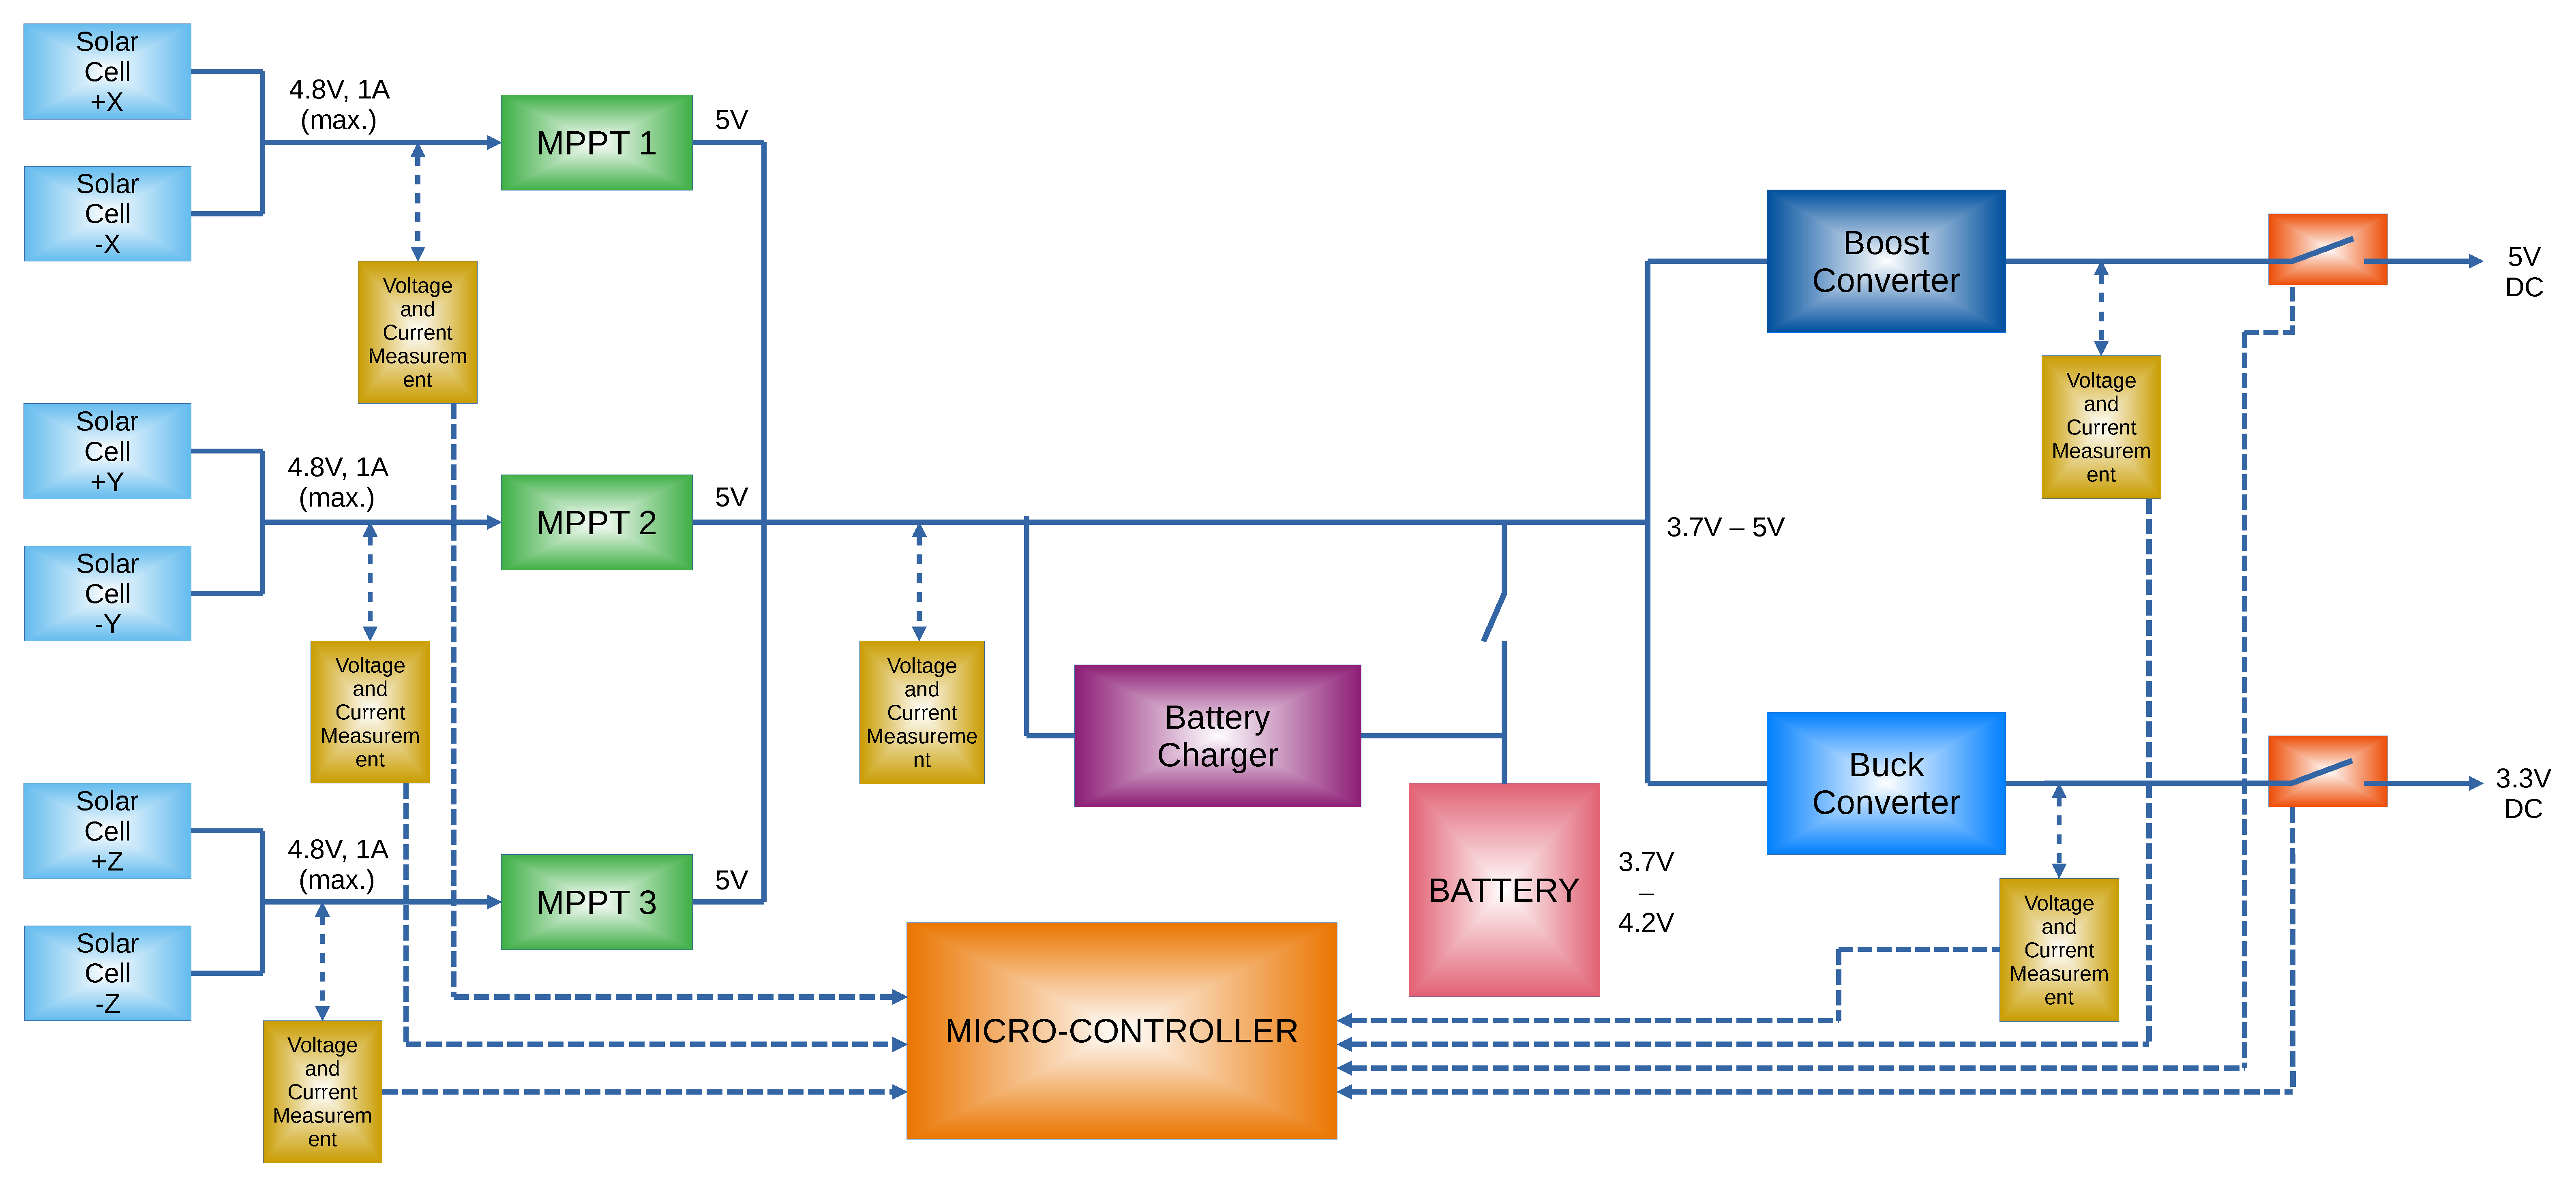
\includegraphics[width=\columnwidth]{diag1.pdf}
	\caption{System Architecture of the CubeSat EPS}
	\label{fig:arch}
\end{figure} 

 \chapter{Component Selection and Design}
\justifying
\section[Solar Panels]{Solar Panels}
 TJ Solar Cell 3G30C - Advanced is selected. This cell is a GaInP/GaAs/Ge on Ge substrate triple junction solar cell. The end-of-life version of the 3G30C solar cell offers best EOL-performance
 values. Connected to the EPS via an external bypass diode protection.
 
 Specifications:
 \begin{itemize}
 	\item Average Open Circuit Voltage: 2.7V
 	\item Maximum Power Point Voltage: 2.41V
 	\item Average Short Circuit Current: 520.2 mA
 	\item Maximum Power Point Current: 504.4mA
 \end{itemize}
It has an average efficiency of 29.8\% at 1353 $W/m^{2}$. This solar cell is excellent for space applications. 
\\
Solar panels are connected in such a way that each side has two cells connected in series.The maximum voltage developed per side is 4.4V and the maximum current that can be generated per side at peak power point is 0.5A.
Panels on opposite sides are connected in parallel.


\section[MPPT Circuit]{Maximum Power Point Tracking Circuit}
The MPPT converter connected to the solar panels increases the efficiency as the
maximum power is transferred from the radiated energy that is on the solar panels.
As each solar panel has different temperatures and incident radiance angles, the
Maximum Power Point (MPP) is also different. So each solar panel has a MPPT
converter to assure that the maximum power available at the solar panels is
transferred independently from their working power points.Since the peak power
point cannot be accurately predicted, many different algorithms exist for finding
the best approximation. The MPPT can be implemented in the EPS using one of three algorithms:
{\bf Perturb and Observe, Incremental Conductance, Constant Voltage}

{\Huge \bf IC ALT}
\section[Battery]{Battery}
The most popular types of batteries use the following materials: Nickel Cadmium
(NiCd), Nickel Metal Hydride (NiMH), Nickel Hydrogen (NiH2), Lithium Ion
(Li-Ion) and Lithium Polymer (Li-Po). The Li-Po and Li-Ion became the standard use in space technology due to their
high energy density (Upto 200 Wh / kg on Li-Po and upto 250 Wh / kg on Li-Ion) and also due to
the number of charging cycles being as high as the NiMH, whilst presenting higher
operating temperatures. 
The Panasonic NCR 18650 GA Li-Ion cell was selected based on the calculation of EOL power, EOL efficiency and due to it's high energy density.
Specifications of Panasonic NCR 18650 GA:
\begin{itemize}
	\item Voltage: 3.7V - 4.2V
	\item Capacity: 3500mAh
	\item 1800 cycles till capacity reduces to 60\%
\end{itemize}
\section[Battery Charger]{Battery Charger}
 The battery also needs a charger to regulate its current and voltage while charging.

 \chapter{Component List}
\begin{table}[h]
	\begin{center}
	\begin{tabular}{|l|l|l|}
		\hline
		{\bf Sl. No.} & {\bf Component} & {\bf Description} \\ \hline
1 & TPS62203 & Buck Converter IC \\ \hline
2 & LTC3426 & Boost Converter IC \\ \hline
3 & BQ25302 & Battery Charger IC \\ \hline
4 & Panasonic NCR 18650 GA & Battery \\ \hline
5 & SPV1040T & MPPT \\ \hline
6 & TJ Solar Cell 3G30C & Solar Cell \\ \hline
7 & STM 32 F401RE & Micro-controller \\ \hline
8 & Resistors &  \\ \hline
9 & Capacitors &  \\ \hline
10 & Inductors &  \\ \hline
11 & PCB &  \\ \hline
	\end{tabular}
\caption{Components Required}
\label{table:3}
	\end{center}
\end{table}
 \chapter{Workplan}
\begin{table}[]
	\begin{tabular}{|l|l|}
		\hline
		\bf{Activites}                                  & \bf{Timeline}            \\ \hline
		Identifying Power Requirements             & Completed           \\ \hline
		Literature Review                          & Completed           \\ \hline
		Architecture Design and Topology selection & Completed           \\ \hline
		Forming Specifications                     & Completed           \\ \hline
		Design and simulation                      & Partly Completed    \\ \hline
		Procurement of components                  & February            \\ \hline
		Fabrication                                & March               \\ \hline
		Testing                                    & April               \\ \hline
		Final Project Report                       & As per KTU Schedule \\ \hline
	\end{tabular}
\end{table}
  

\chapter{Testing}

\section{Variable DC load using MOSFET}
To test the efficiency of the demo boards, different tests like line regulation, load regulation etc have to be conducted. For line regulation, at a certain constant load, we should create a voltage values table and get the efficiency curve. For that, we need different values of resistance (load). Instead of using resistance, we could use a MOSFET for simulating various load conditions. Since we don’t need any higher loads to test the demo boards, a circuit that simulate a load precisely for values from 0 to 2A and with a precision of 0.01A will do the job.

\begin{figure}[h]
	\centering
	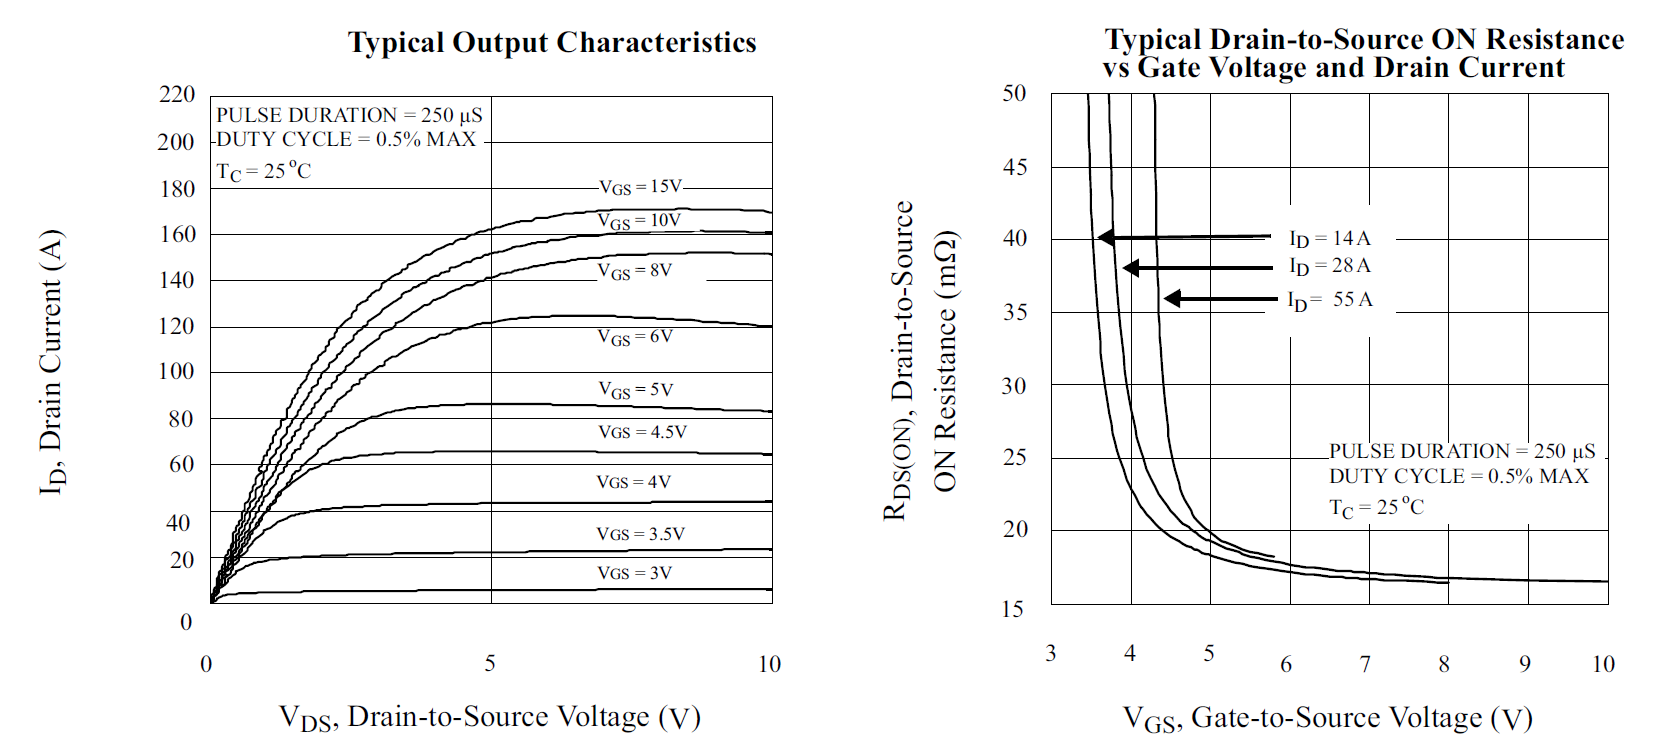
\includegraphics[width=\columnwidth]{IMGS/MosfetChara.jpg}
	\caption{Mosfet characteristics}
	\label{fig:arch}
\end{figure} 

IRFZ44 is the MOSFET used to implement this circuit. It has a Vds on voltage of 10V. A potentiometer is used to control the gate source voltage and the circuit to be tested is connected between the drain and source terminals. By varying the gate voltage, the drain source conduction can be controlled. The drain source voltage and current increases proportionally with increase in gate voltage and thus the setup acts as a resistive load. The setup implementation is as follows:-
% The working of the circuit is simple. The MOSFET is controlled by voltage on its gate. Till the voltage between gate and source (Vgs) is not higher than a certain value called Vth, the MOSFET is disabled, so no current will be flowing between drain and source. After Vth, the MOSFET starts a current flow and the value of this current will get higher as Vgs increases till a certain value where the MOSFET is fully on. So, by varying the voltage at the gate we change the current flow and by that we can simulate the load value. 
%\\ \\

% \\ \\	
% But there is no relation between the voltage at the gate and the current value. For that we add a 1 ohms 5W resistor at the source of the MOSFET. Since we know for sure the resistor is 1 ohm, for example, when 1 amp is flowing, we will have 1V voltage drop on this resistor and we can measure that with a precise ADC. In this way we can know the current value.
% \\ \\
% Since we can't know what voltage to put at the MOSFET gate in order to get any current value, we use the OPAMP and this will do that for us automatically. Let's say we want a current flow of 1A. All we need is to get a 1V voltage drop on the 1ohm power resistor. That point, as you can see in the schematic, is connected to the negative input of the OPAMP. We know that the OPAMP will do all that is necessary to have the same voltage on the input V- as on input V+. So if we place 1V at V+, the OPAMP will change the voltage at the MOSFET gate till the voltage on the resistor is 1V as well, since that point is connected at input V- of the OPAMP. So, just like that, we can get any value of current that we want.
% \\ \\
% \begin{figure}[h]
% 	\centering
% 	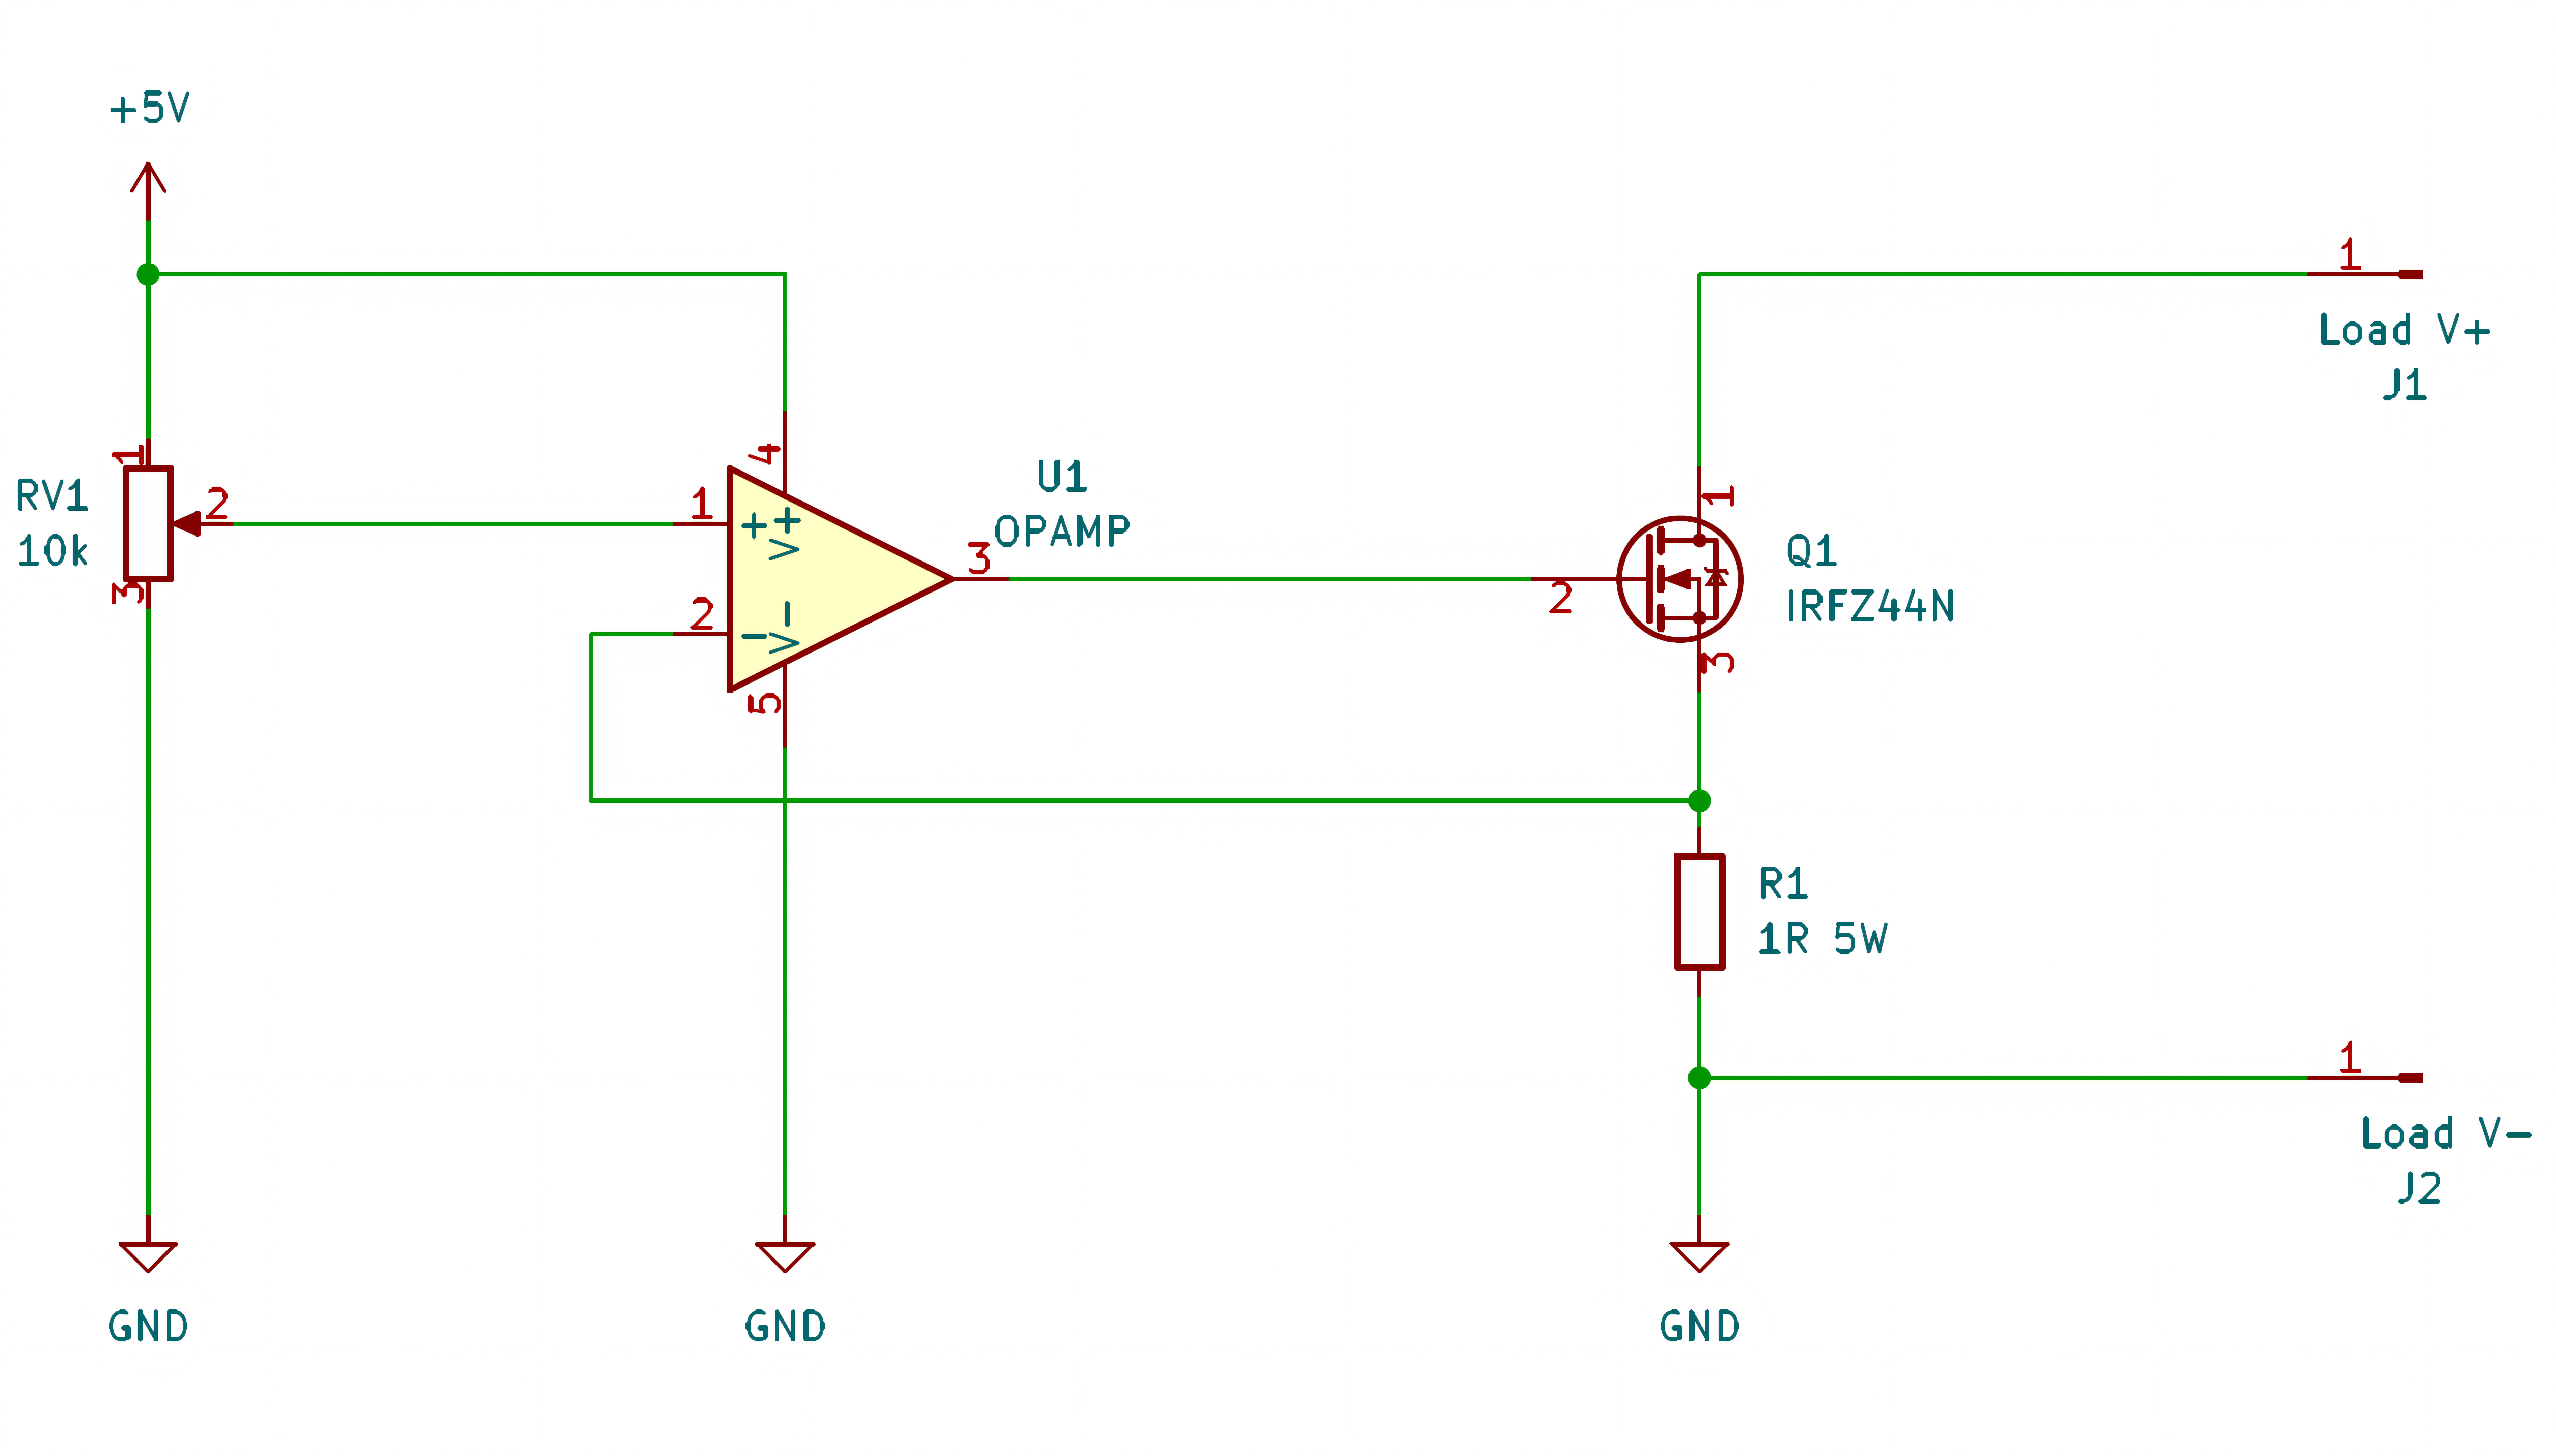
\includegraphics[width=\columnwidth]{IMGS/LoadSchematic.jpg}
% 	\caption{Variable DC load schematics}
% 	\label{fig:arch}
% \end{figure} 
% \\ \\	
\section{VirtualBench}

The VirtualBench is an instrument which combines a mixed-signal oscilloscope with an arbitrary waveform generator, a digital multi-meter, a programmable DC power supply, and digital I/O. The all-in-one features are simple, convenient, and provide more efficient circuit design, debugging, and validation, and the included software lets us to view all measurements on a single screen.

\begin{figure}[H]
	\centering
	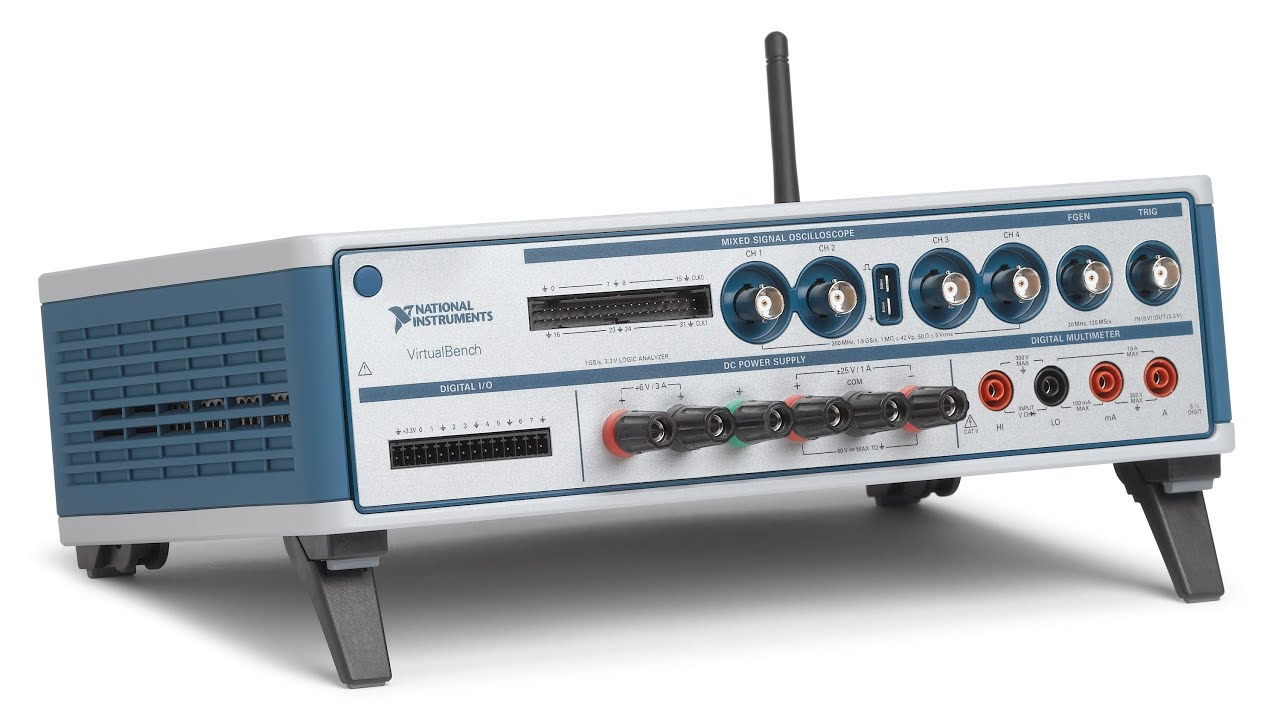
\includegraphics[width=0.8\columnwidth]{IMGS/TestSetupPics/NIVirtualBench.png}
	\caption{VirtualBench}
	\label{fig:arch}
\end{figure}
\pagebreak
\section{Testing of DC/DC converters}
DC/DC converters have a specified input voltage operating range. To confirm the DC/DC converter works properly over the entire range of input voltages, they are tested using an adjustable or programmable dc source to provide the input voltage. A dc electronic load is used on the output of the DC/DC converter to set the output load current and simulate the device that the DC/DC converter would power.

% \subsection{Input turn-on, input turn-off voltage levels and timing test}

% To test the minimum input voltage turn-on level, the DC/DC converter is turned on using the nominal input voltage while using the electronic load to apply the maximum rated output current or power. The input voltage is then reduced until the unit output begins to drop or the minimum input voltage setting is met.
% \\ \\
% To confirm the DC/DC converter would turn on with a maximum load on the output, the input voltage would be set to the minimum and toggled off and back on while measuring the output voltage and current. The output voltage and ripple and noise may also be measured to see if the lower input voltage setting has any effect on the output stability or ripple.
% \\ \\
% Additionally, this setup can be used to test and measure the turn-on time, turn-off time, and hold-up times. An oscilloscope is used for the ripple and for periodic and random deviation (PARD) measurements.
%\\ \\
\begin{figure}[H]
	\centering
	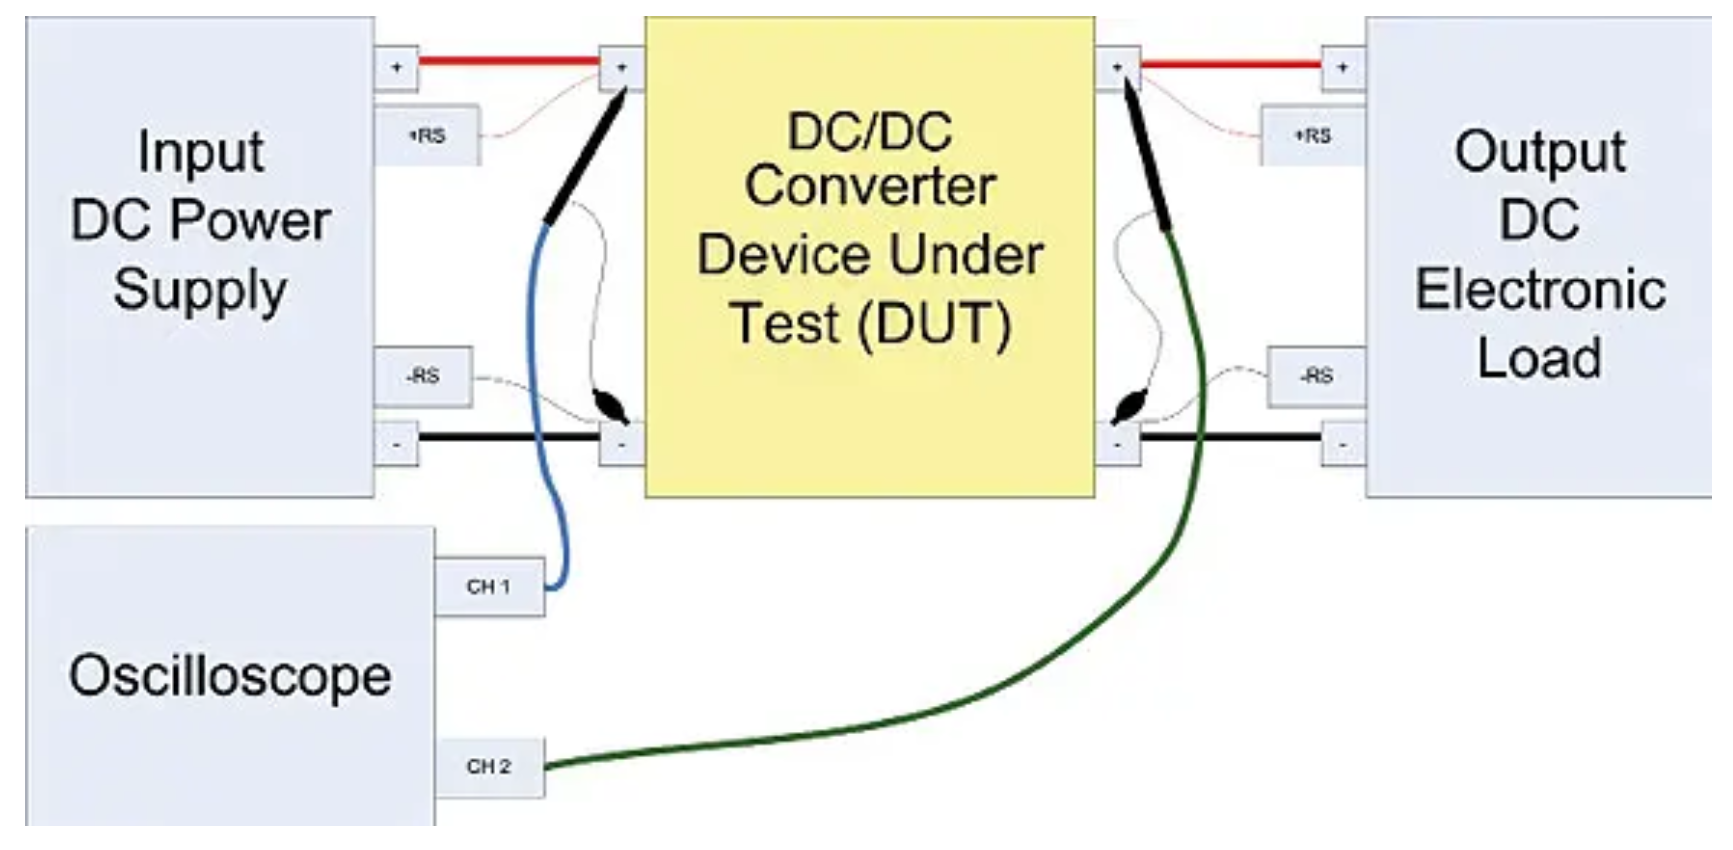
\includegraphics[width=\columnwidth]{IMGS/DCDCconverterTestSetup.jpg}
	\caption{Test setup}
	\label{fig:arch}
\end{figure} 

\begin{figure}[H]
	\centering
	\includegraphics[width=0.9\columnwidth]{IMGS/TestSetupPics/TESTPIC_REG_MODULE.jpg}
	\caption{Regulation module test setup}
	\label{fig:arch}
\end{figure}
% \\ \\	
% % Turn-on time indicates the period from the time at which the minimum input voltage is applied to the time the output voltage is within the output regulation limits. Turn-off time indicates when the input voltage drops below the specified minimum and the output turns off or drops to zero volts.
% \\ \\
% % \begin{figure}[h]
% % 	\centering
% % 	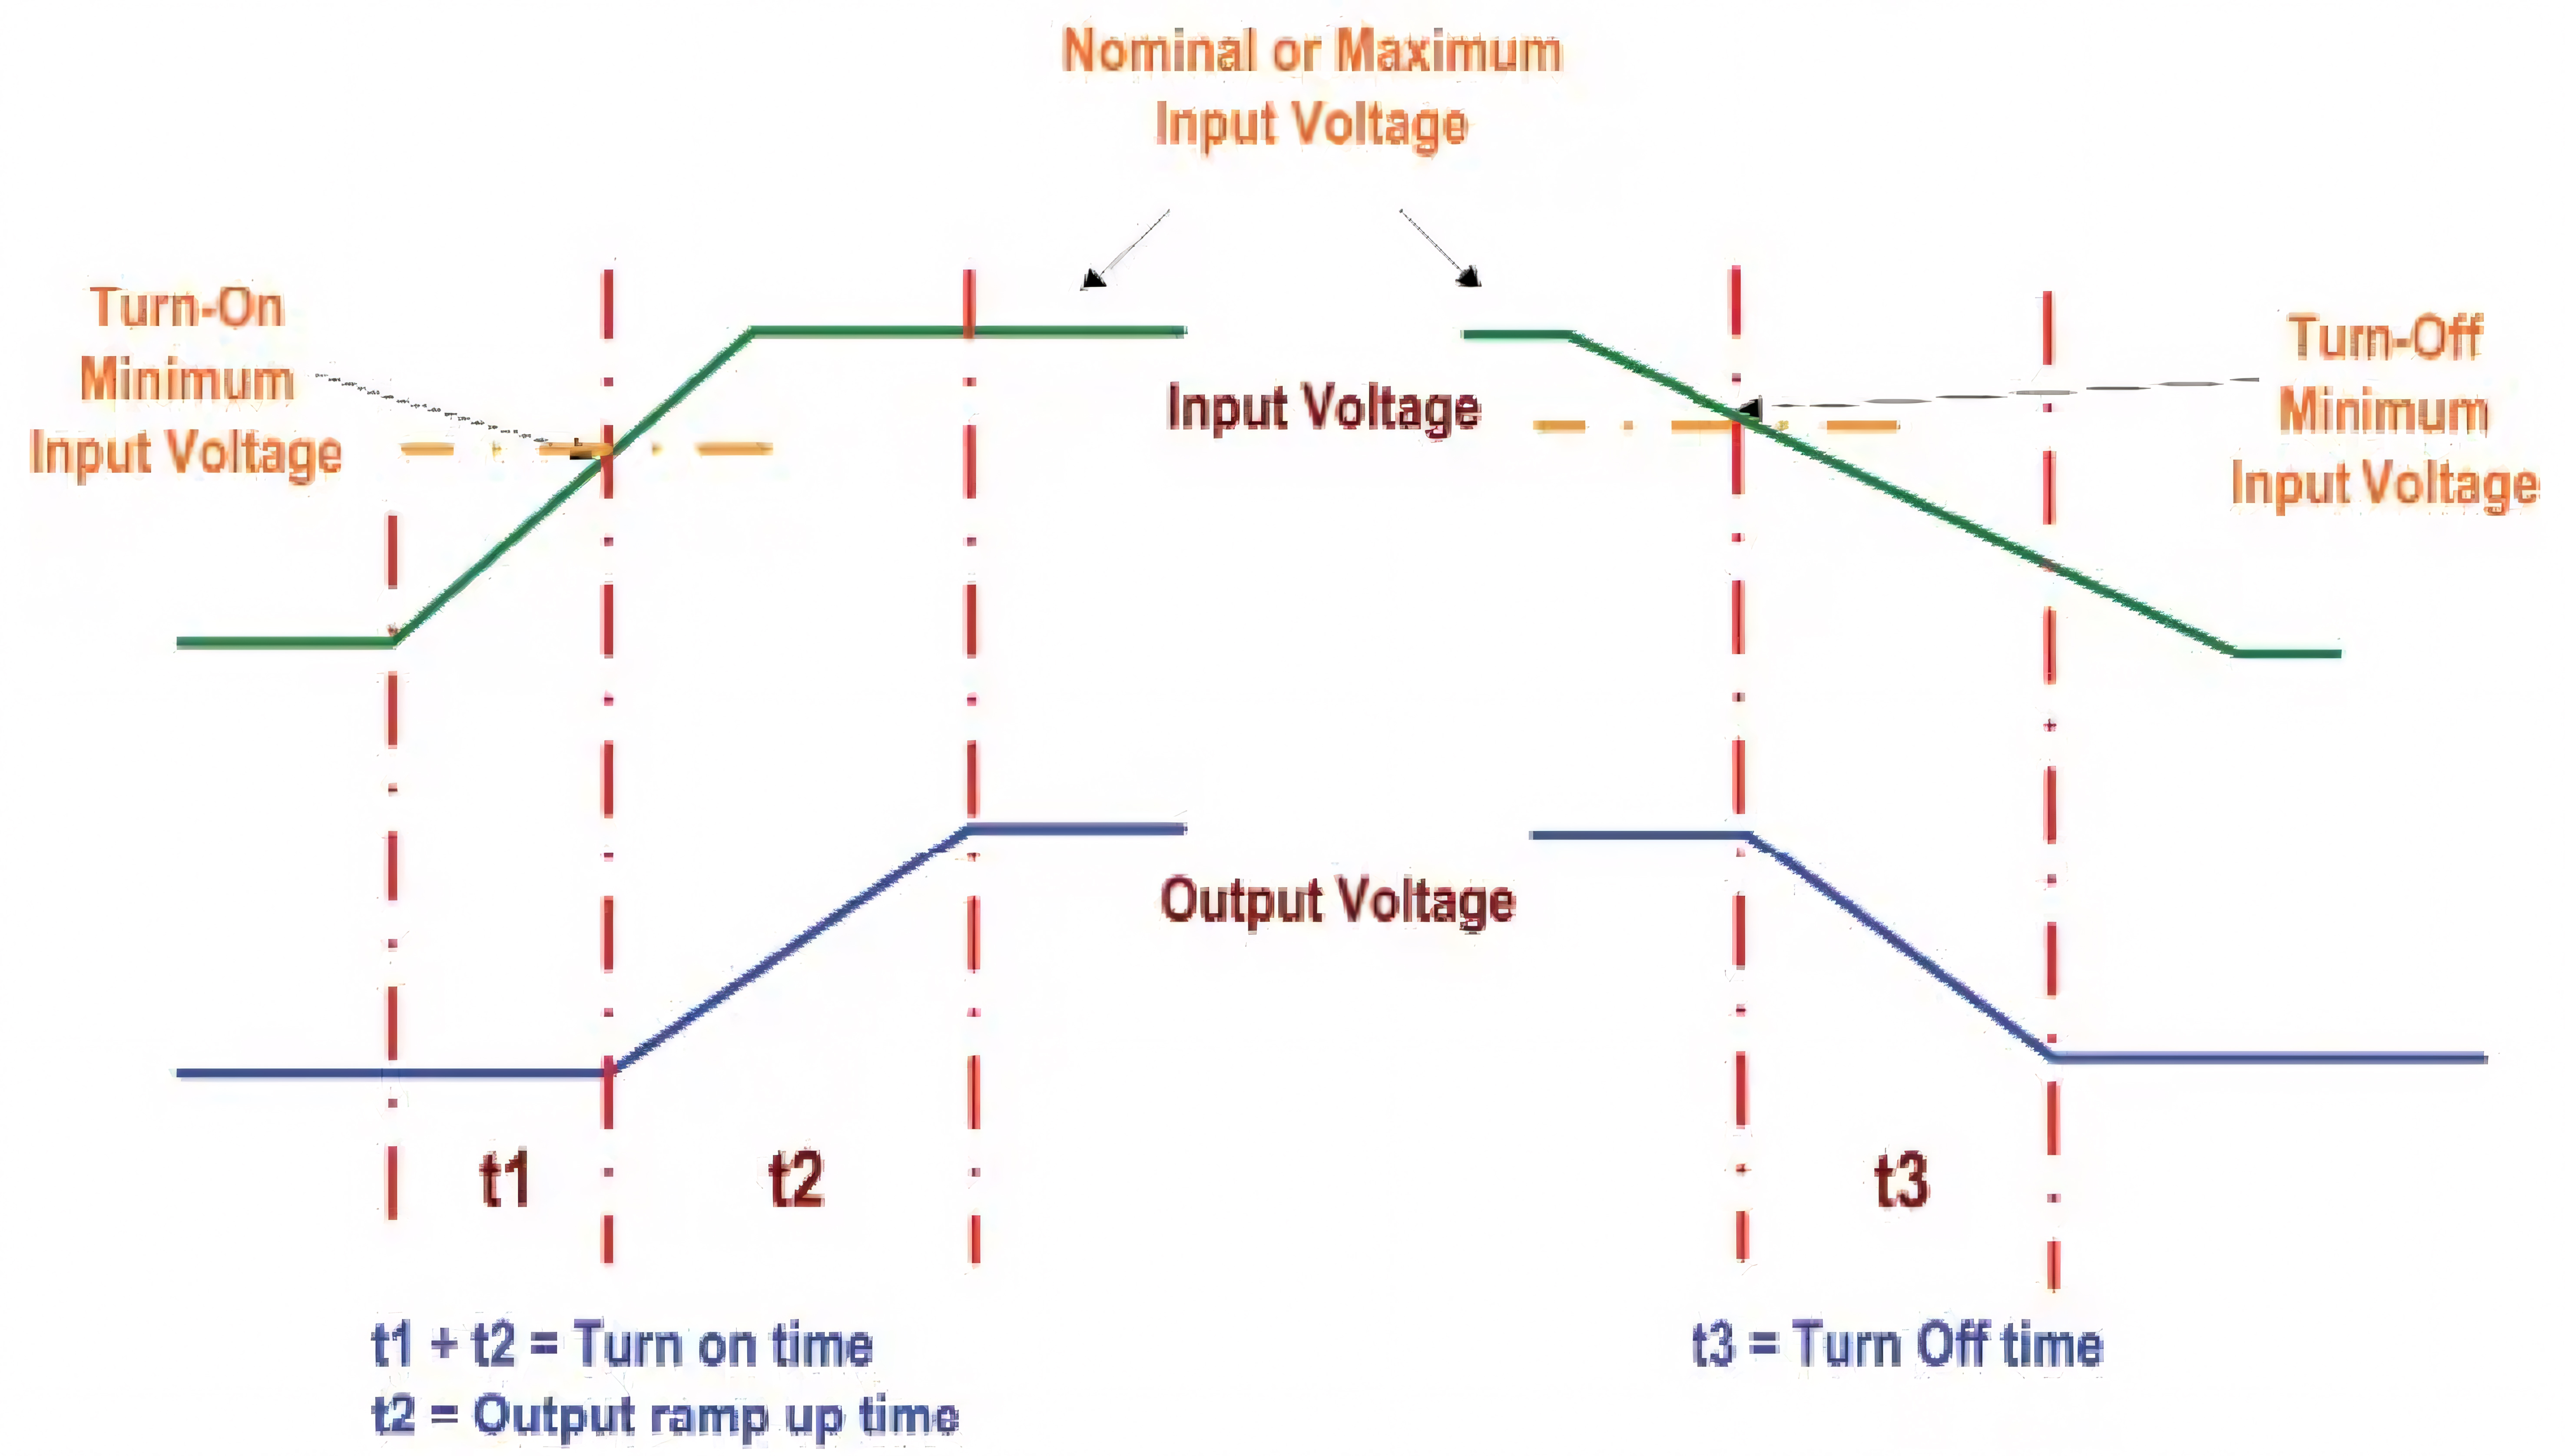
\includegraphics[width=\columnwidth]{IMGS/TurnOnTurnOff.jpg}
% % 	\caption{Turn-on, Turn-off characteristics}
% % 	\label{fig:arch}
% % \end{figure} 
% \\ \\	
% % The hold-up timing test can use the same setup as the input turn-on and turn-off test. Hold-up timing indicates the time from when the input drops below the minimum input voltage and the output voltage drops below its minimum regulated output tolerance. This test also indicates how well the output of the DC/DC converter can continue to operate despite short interrupts and drops in the input voltage. Some DC/DC converters have an input fault detection signal. If so, this signal can be used to trigger the test.
% \\ \\
% % \begin{figure}[h]
% % 	\centering
% % 	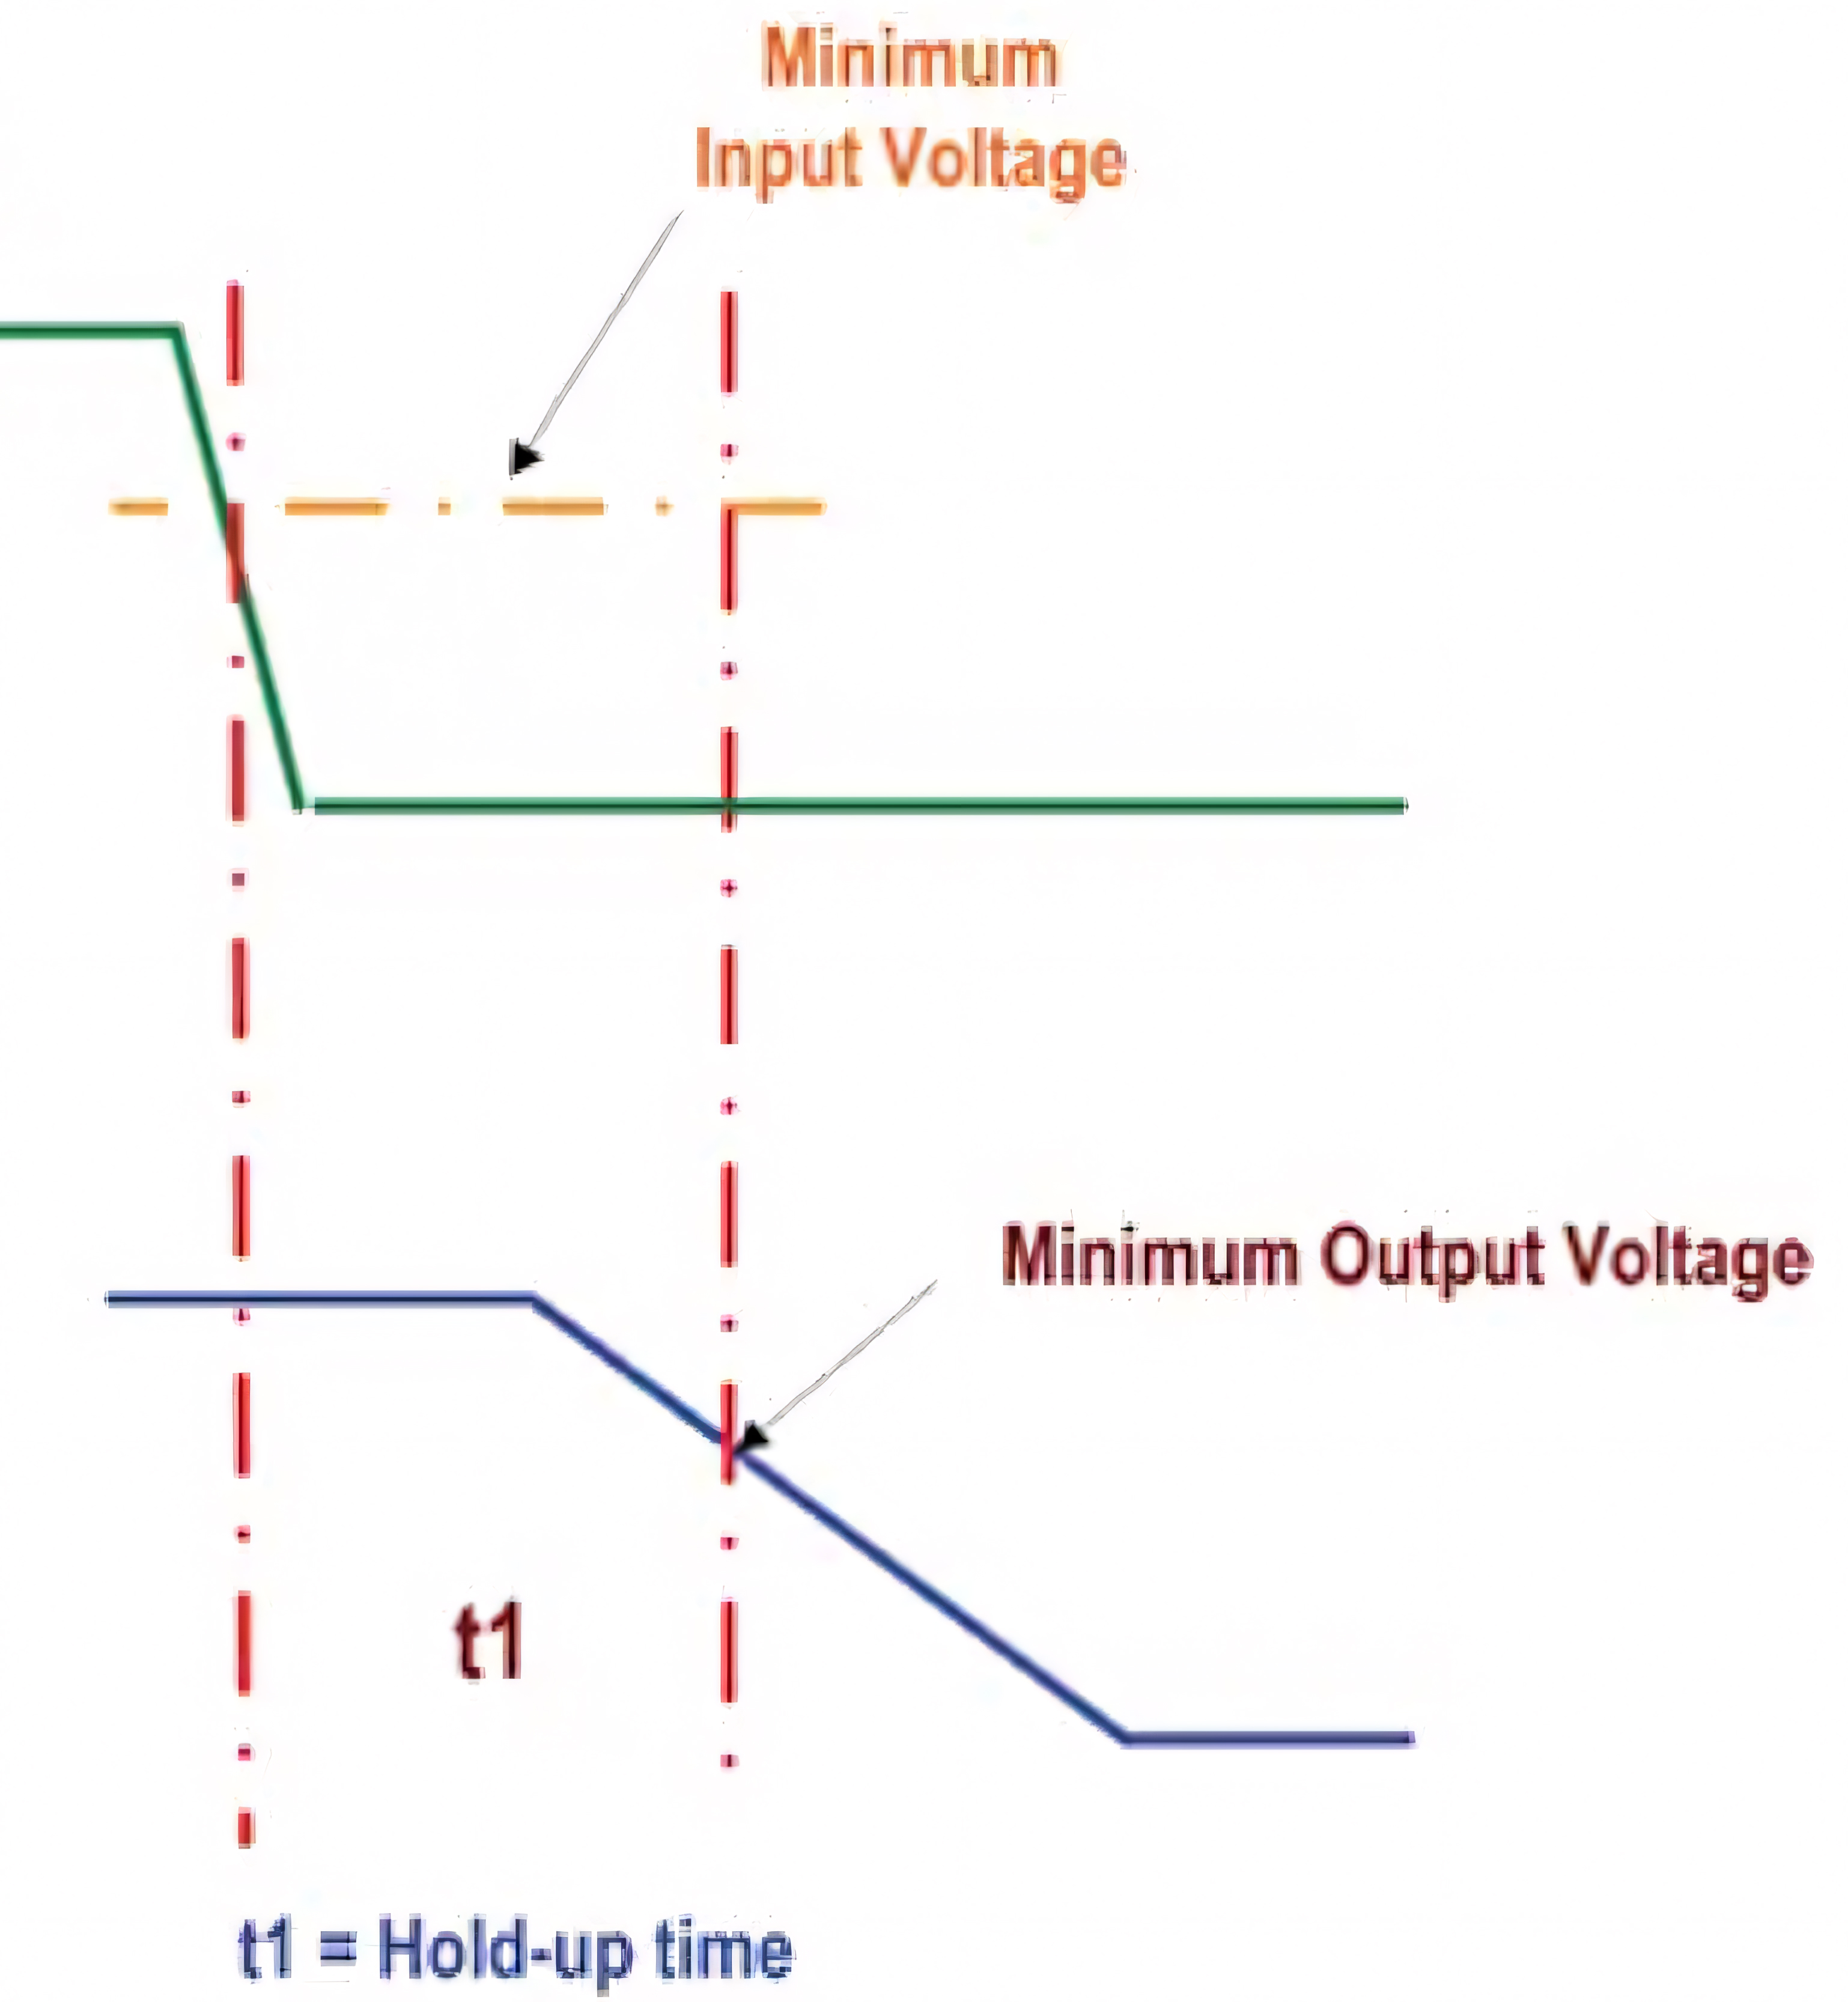
\includegraphics[width=140pt]{IMGS/HoldUpTimeTest.jpg}
% % 	\caption{Hold-up time characteristics}
% % 	\label{fig:arch}
% % \end{figure} 
% \\ \\
\subsection{Output line regulation}

This test confirms that the output voltage stays within specified regulation limits when the input voltage varies from minimum to maximum operating voltage, as defined in the DC/DC converter specification. During this test the output load is usually set to nominal or maximum current as specified.
\\ \\
The output line regulation test involves monitoring the output voltage and recording the total voltage deviation while varying the input voltage from its minimum to maximum specified limits. Some specifications show the output tolerance as a voltage (i.e. 3.3 Vdc ± 0.02 V) or as a percentage (i.e. 3.3 V ± 0.5\%).
\\ \\
Output regulation $R_{o}$ is calculated as a percentage and given by the equation:
\\ \\
\hspace*{5cm}$R_{o}$ = $\left | \frac{V_{omax}-V_{omin}}{V_{onom}} \right | \times 100$
\\ \\
where:
$V_{omax}$ = Vout at Vin max; 
$V_{omin}$ = Vout at Vin min; and
$V_{onom}$ = Vout nominal.

\begin{figure}[H]
	\centering
	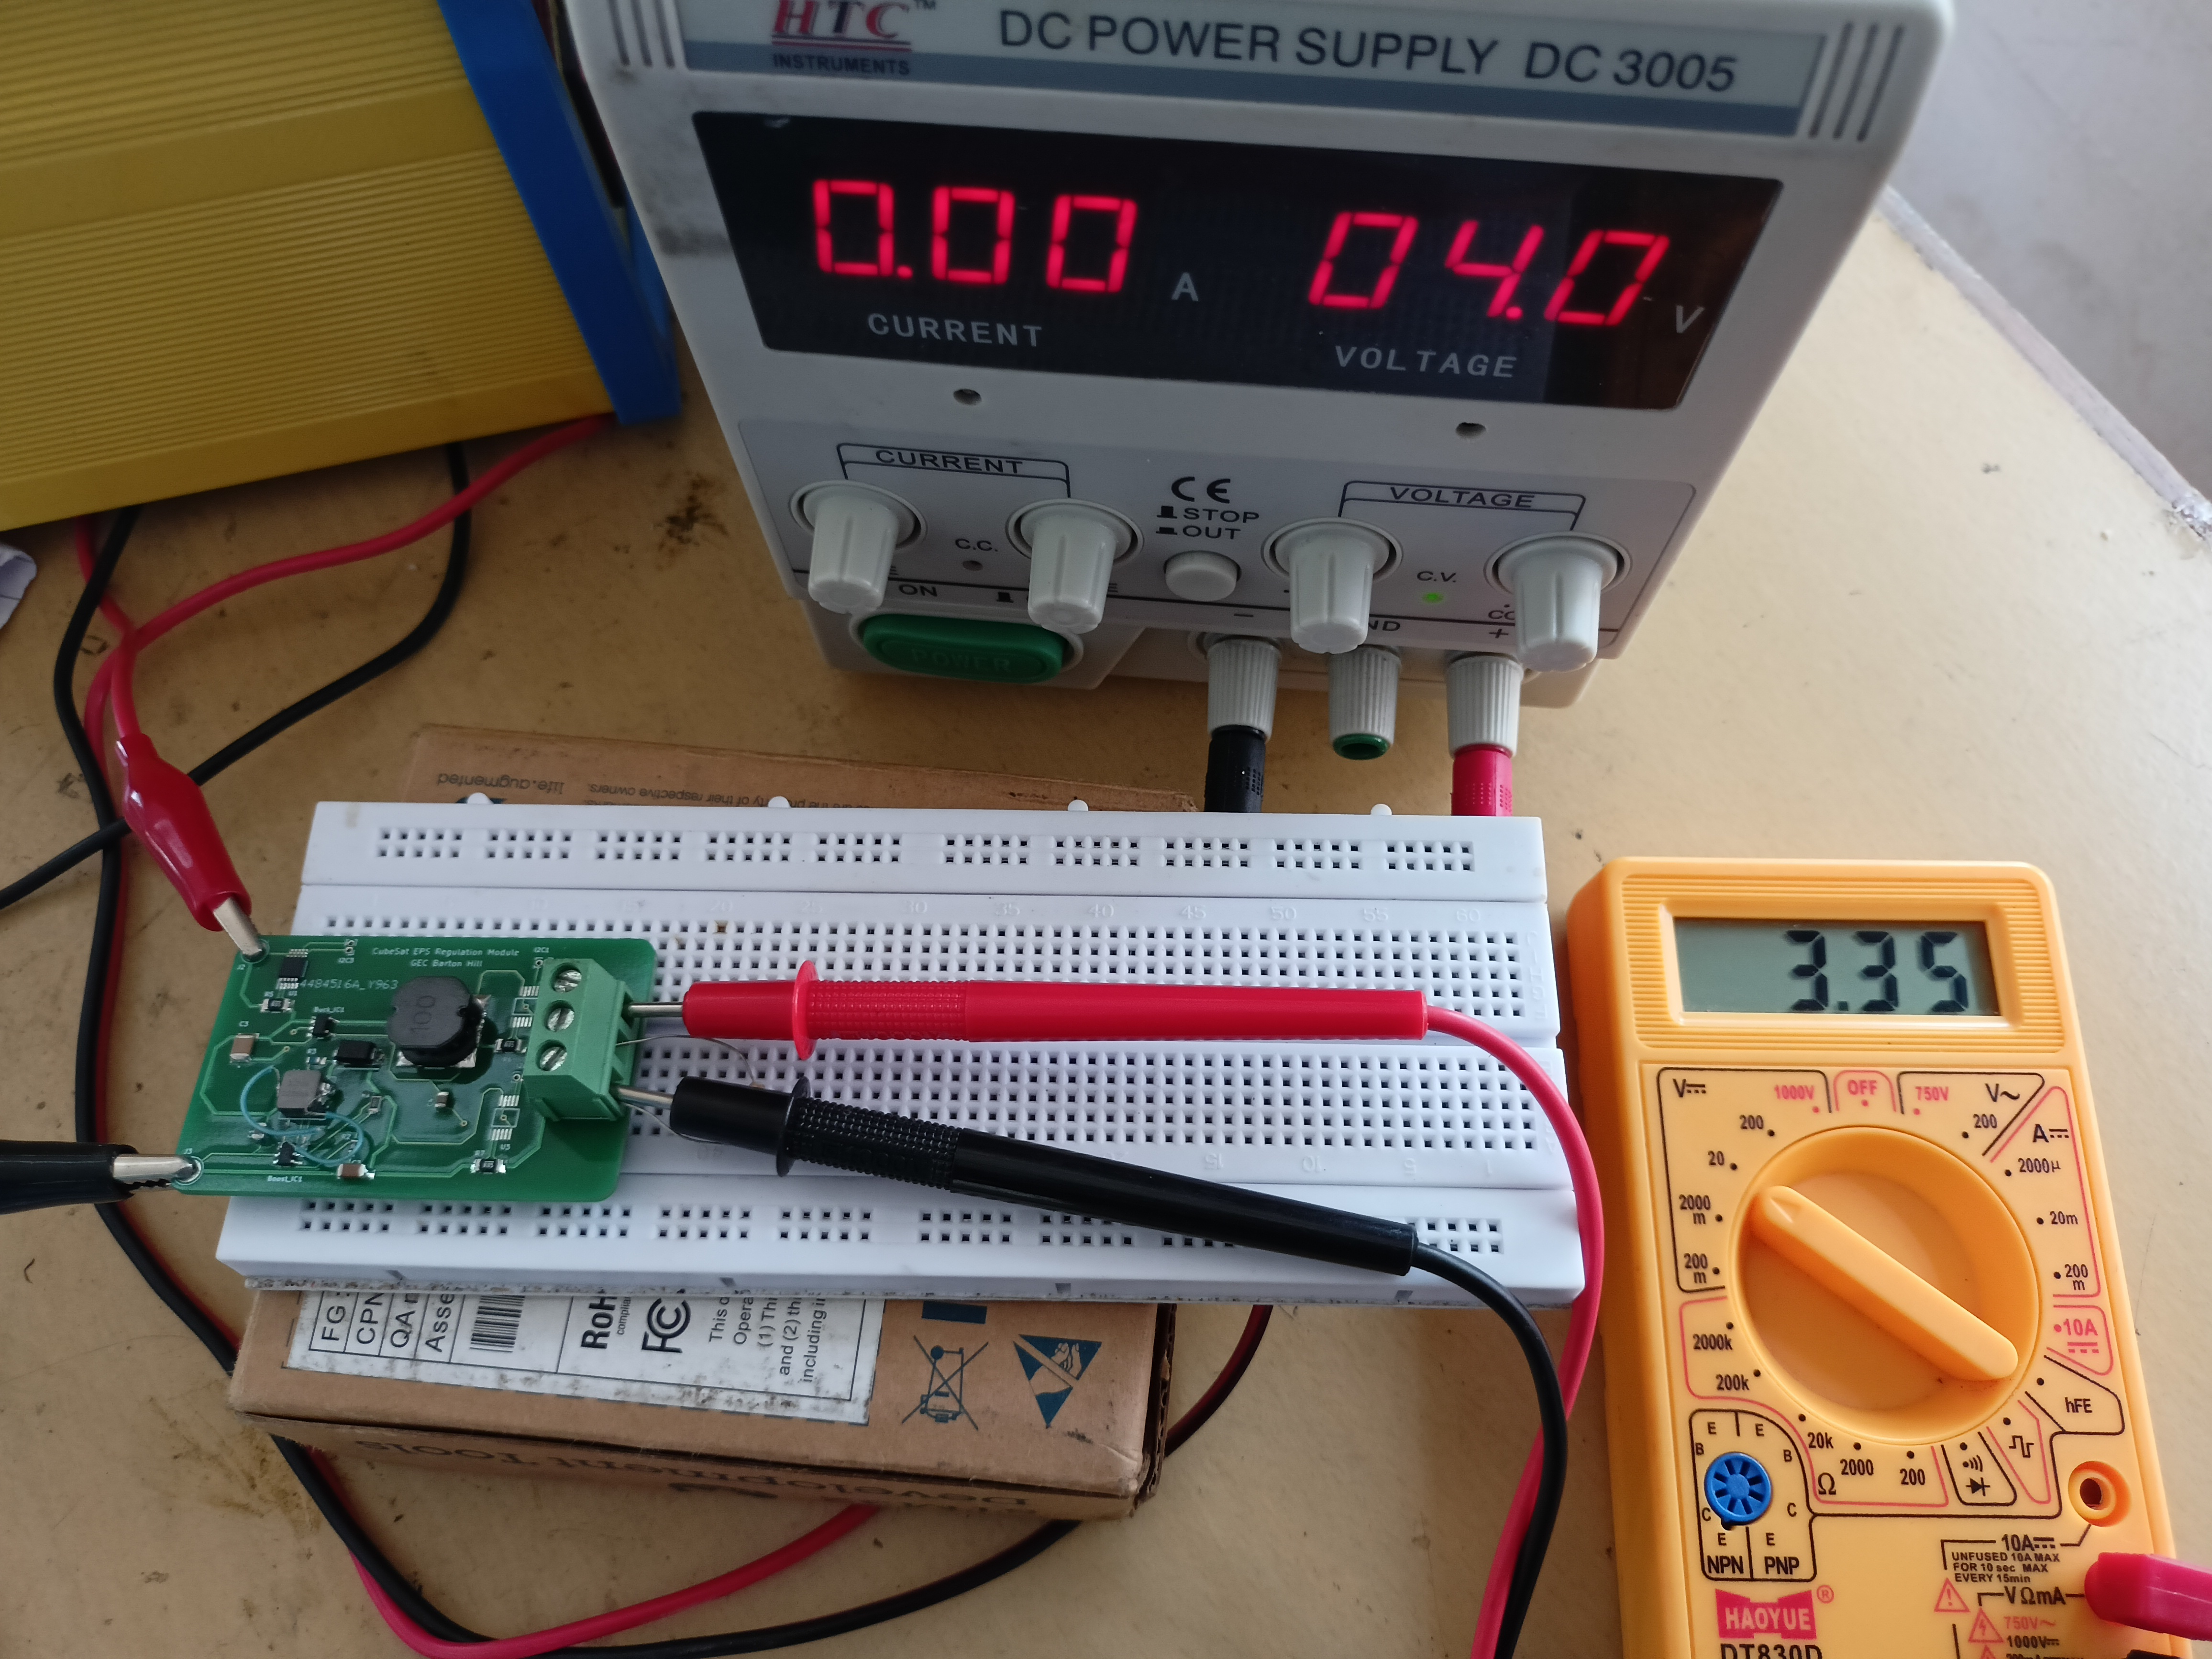
\includegraphics[width=0.9\columnwidth]{IMGS/TestSetupPics/Buck_out.jpg}
	\caption{Testing buck converter in 3.3V rail}
	\label{fig:arch}
\end{figure}

\pagebreak

\begin{table}[H]
\centering
\begin{tabular}{|l|l|l|l|}
\hline
Vin (Volt) & Vout (Volt) & Iin (A) & Efficiency \\ \hline
3.6        & 3.25        & 0.19    & 95.02924   \\ \hline
4          & 3.25        & 0.17    & 95.58824   \\ \hline
4.2        & 3.21        & 0.17    & 89.91597   \\ \hline
4.6        & 3.25        & 0.16    & 88.31522   \\ \hline
5          & 3.22        & 0.15    & 85.86667   \\ \hline
5.5        & 3.2         & 0.13    & 89.51049   \\ \hline
6          & 3.2         & 0.12    & 88.88889   \\ \hline
\end{tabular}
\caption{Buck output line regulation at full load (200mA)}
\label{table:4}
\end{table}
\\
\begin{figure}[H]
	\centering
	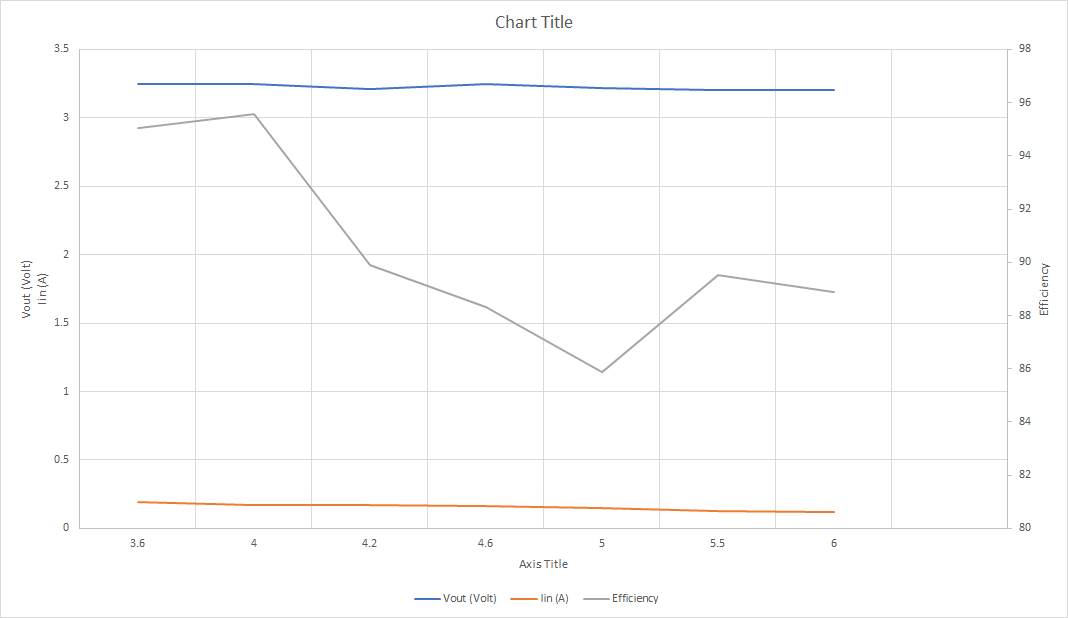
\includegraphics[width=\columnwidth]{IMGS/Buck output line regulation at full load (200mA).png}
	\caption{Buck output line regulation at full load (200mA)}
	\label{fig:arch}
\end{figure}

\begin{table}[H]
\centering
\begin{tabular}{|l|l|}
\hline
Vin (Volt) & Vout (Volt) \\ \hline
3.6        & 3.3         \\ \hline
4          & 3.35        \\ \hline
4.2        & 3.35        \\ \hline
4.6        & 3.35        \\ \hline
5          & 3.35        \\ \hline
5.5        & 3.35        \\ \hline
6          & 3.35        \\ \hline
\end{tabular}
\caption{Buck output line regulation at no load}
\label{table:4}
\end{table}
\\
\begin{figure}[H]
	\centering
	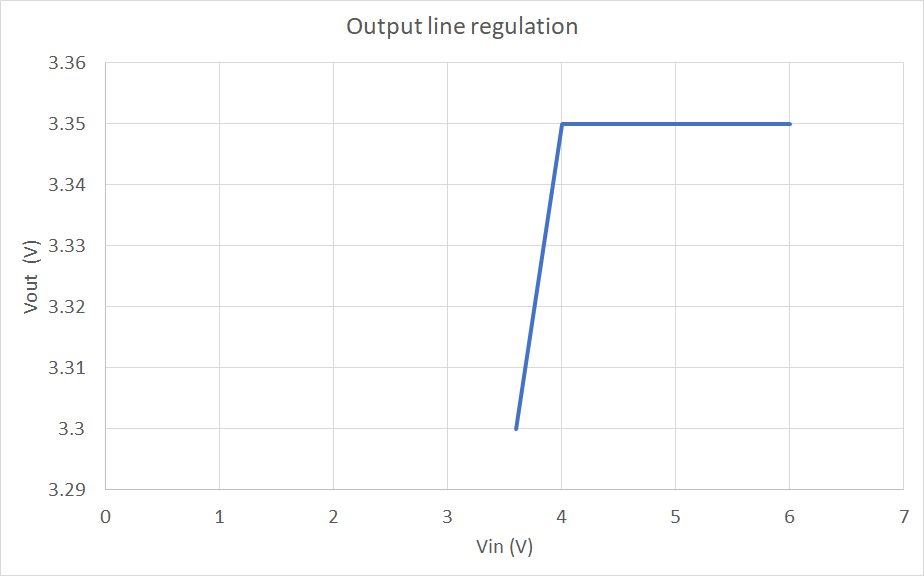
\includegraphics[width=\columnwidth]{IMGS/Buck line regulation at no load.png}
	\caption{Buck output line regulation at no load}
	\label{fig:arch}
\end{figure}
\begin{table}[H]
\centering
\begin{tabular}{|l|l|l|l|}
\hline
Vin (Volt) & Vout (Volt) & Iin (A) & Efficiency \\ \hline
3.6        & 3.25        & 0.16    & 84.63542   \\ \hline
4          & 3.25        & 0.14    & 87.05357   \\ \hline
4.2        & 3.26        & 0.13    & 89.56044   \\ \hline
4.6        & 3.27        & 0.12    & 88.8587    \\ \hline
5          & 3.28        & 0.11    & 89.45455   \\ \hline
5.5        & 3.29        & 0.1     & 89.72727   \\ \hline
6          & 3.27        & 0.09    & 90.83333   \\ \hline
\end{tabular}
\caption{Buck output line regulation at half load(150mA)}
\label{table:4}
\end{table}
\\
\begin{figure}[H]
	\centering
	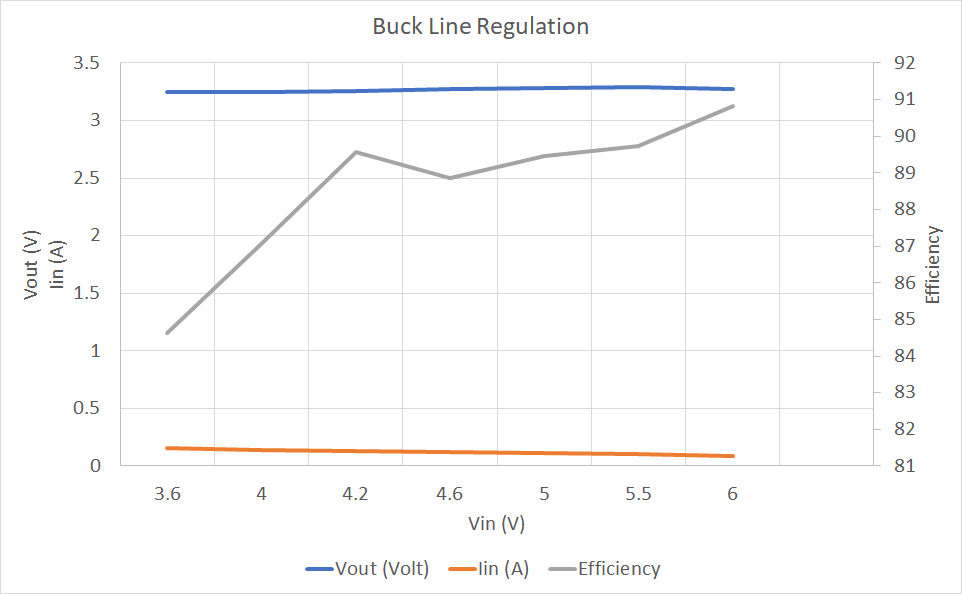
\includegraphics[width=\columnwidth]{IMGS/Buck output line regulation at half load (150mA).png}
	\caption{Buck output line regulation at half load(150mA)}
	\label{fig:arch}
\end{figure}
\pagebreak

\begin{table}[H]
\centering
\begin{tabular}{|l|l|l|l|}
\hline
Vin (Volt) & Iin (A) & Vout (Volt) & Efficiency \\ \hline
3.6        & 1.09    & 3.7         & 70.71865   \\ \hline
4.2        & 1.24    & 4.47        & 64.37212   \\ \hline
4.8        & 1.2     & 4.8         & 66.66667   \\ \hline
\end{tabular}
\caption{Boost output line regulation at full load(750mA)}
\label{table:4}
\end{table}
\\

\begin{figure}[H]
	\centering
	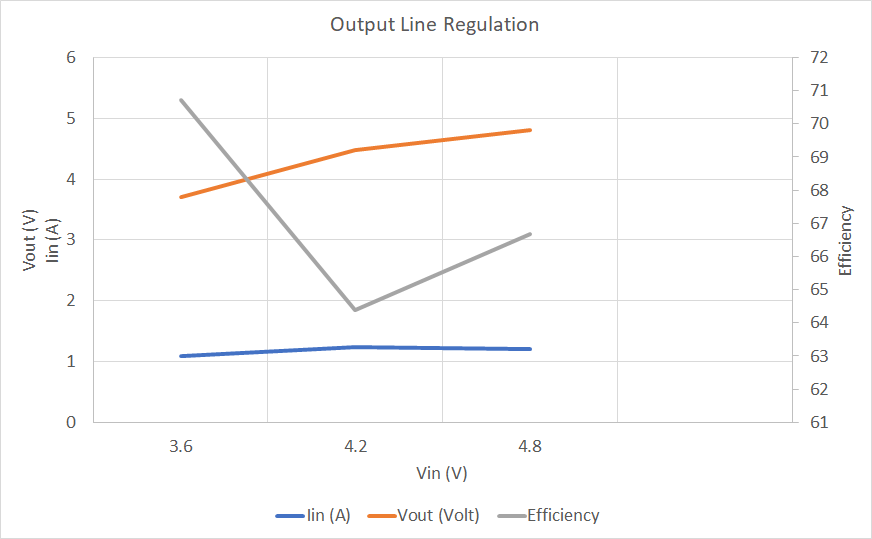
\includegraphics[width=\columnwidth]{IMGS/Boost output regulation at full load (750mA).png}
	\caption{Boost output line regulation at full load (750mA)}
	\label{fig:arch}
\end{figure}
\pagebreak

\begin{table}[H]
\centering
\begin{tabular}{|l|l|l|l|}
\hline
Vin (Volt) & Iin (A) & Vout (Volt) & Efficiency \\ \hline
3.3        & 0.84    & 4.93        & 71.13997   \\ \hline
4.2        & 0.68    & 5.13        & 71.84874   \\ \hline
5          & 0.65    & 5.05        & 62.15385   \\ \hline
\end{tabular}
\caption{Boost output line regulation at half load(400mA)}
\label{table:4}
\end{table}
\\
\begin{figure}[H]
	\centering
	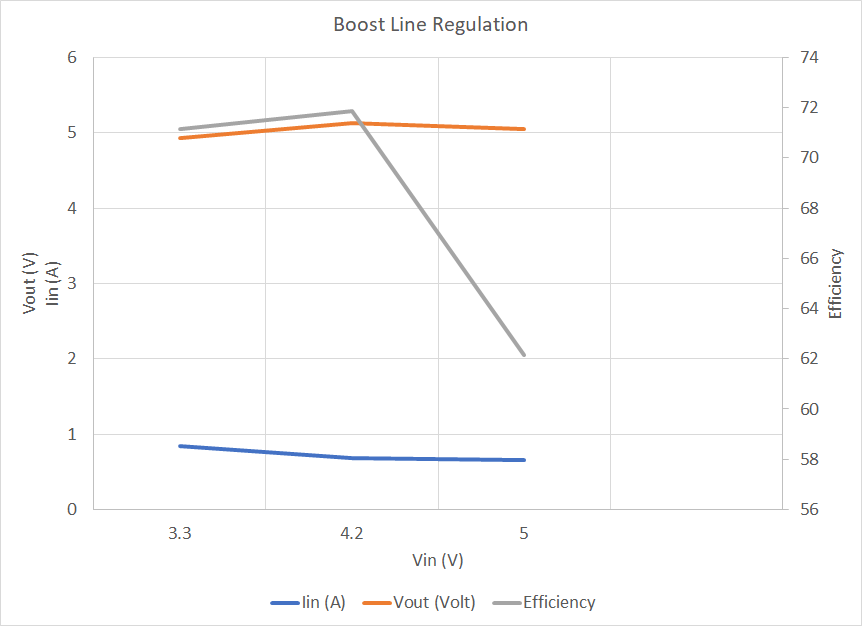
\includegraphics[width=\columnwidth]{IMGS/Boost output line regulation at half load (400mA).png}
	\caption{Boost output line regulation at half load (400mA)}
	\label{fig:arch}
\end{figure}
\pagebreak

\begin{figure}[H]
	\centering
	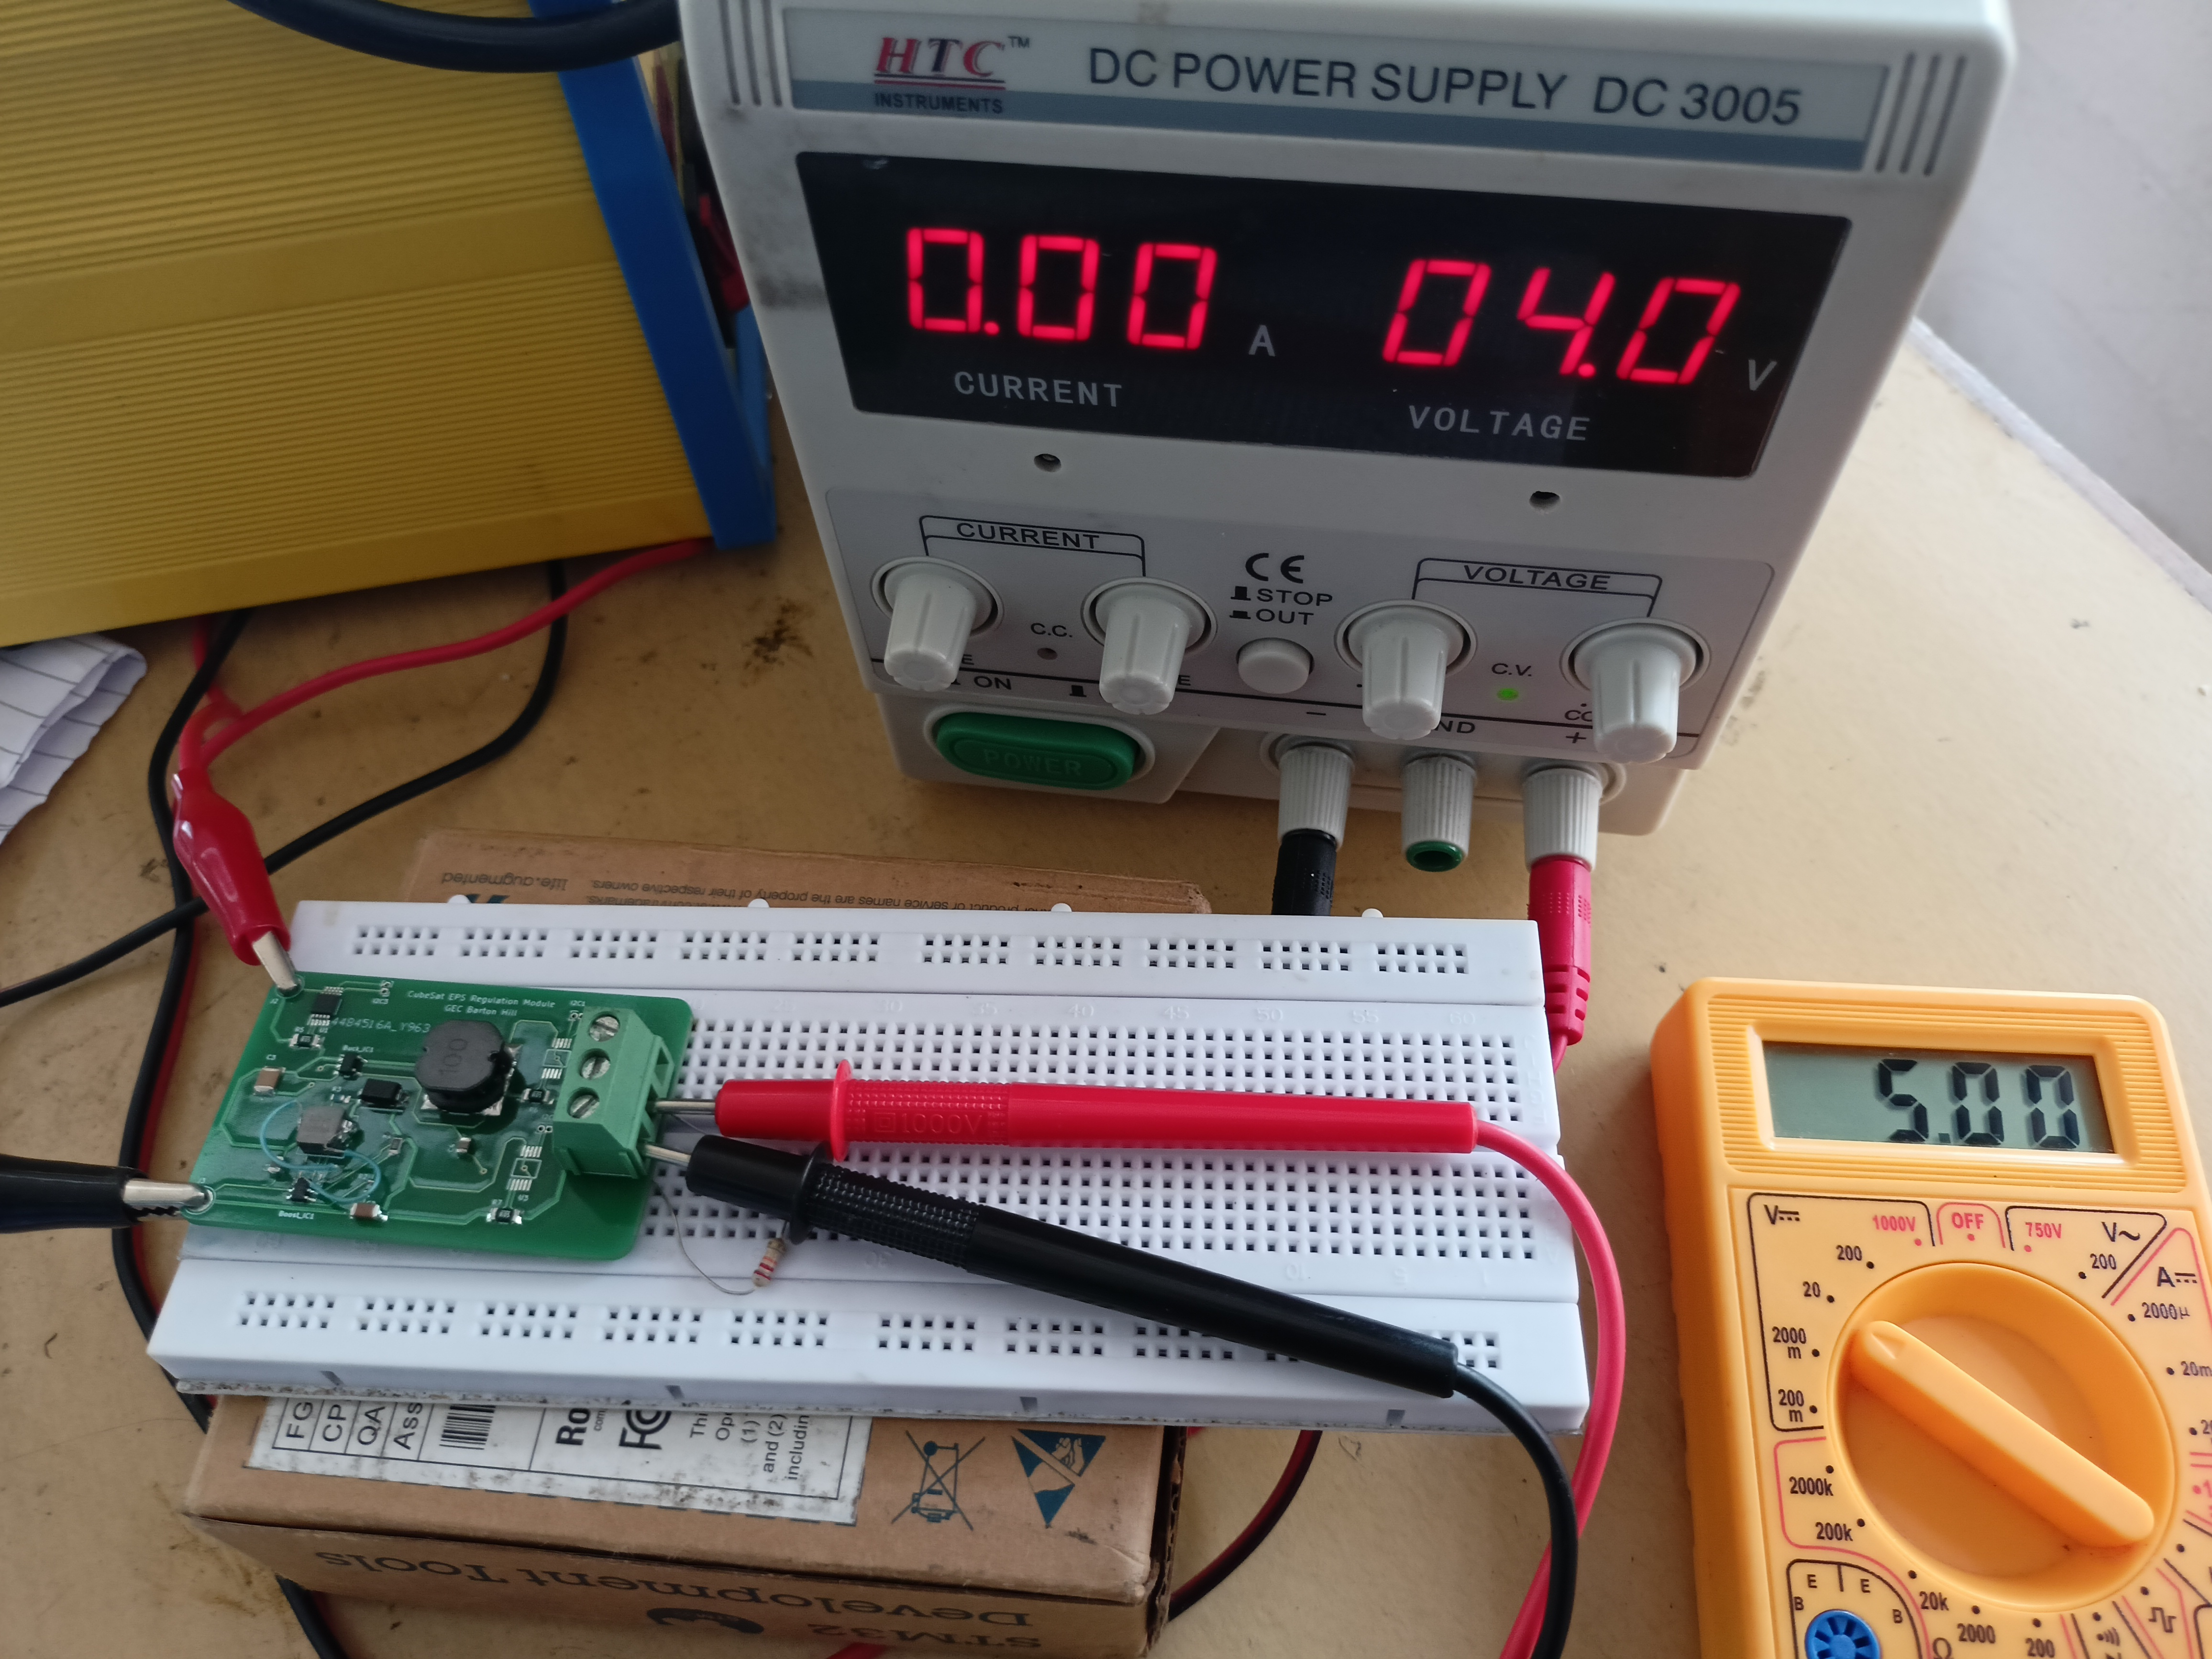
\includegraphics[width=\columnwidth]{IMGS/TestSetupPics/Boost_out.jpg}
	\caption{Testing of boost converter in 5V rail}
	\label{fig:arch}
\end{figure}
\subsection{Output load regulation} 
The output load regulation test ensures the DC/DC converter output voltage stays within the specified regulation tolerance. Here, the change in output voltage is recorded while load is varied from minimum to maximum current. This delta voltage is used to calculate the percentage of deviation which is compared to the specified load regulation limits. Load regulation $L_{r}$ is calculated as a percentage from the equation:
\\ \\
\hspace*{5cm}$L_{r}$ = $\left | \frac{V_{oio}-V_{oim}}{V_{onom}} \right | \times 100$
\\ \\
Where:
$V_{oio}$ = Vout at Iout max; 
$V_{oim}$ = Vout at Iout min; and
$V_{onom}$ = Vout nominal.
\pagebreak
\begin{table}[H]
\centering
\begin{tabular}{|l|l|l|l|}
\hline
Iout (mA) & Vout (Volt) & Iin(A) & Efficiency \\ \hline
50        & 4.94        & 0.09   & 76.23457   \\ \hline
100       & 4.94        & 0.18   & 76.23457   \\ \hline
150       & 4.91        & 0.28   & 73.06548   \\ \hline
200       & 4.89        & 0.39   & 69.65812   \\ \hline
250       & 4.87        & 0.49   & 69.01927   \\ \hline
300       & 4.87        & 0.61   & 66.53005   \\ \hline
350       & 4.87        & 0.77   & 61.4899    \\ \hline
400       & 4.86        & 0.86   & 62.7907    \\ \hline
450       & 4.7         & 0.99   & 59.34343   \\ \hline
500       & 4.44        & 0.92   & 67.02899   \\ \hline
550       & 4.6         & 1.01   & 69.58196   \\ \hline
\end{tabular}
\caption{Boost load regulation at 3.6V Vin}
\label{table:4}
\end{table}
\\
\begin{figure}[H]
	\centering
	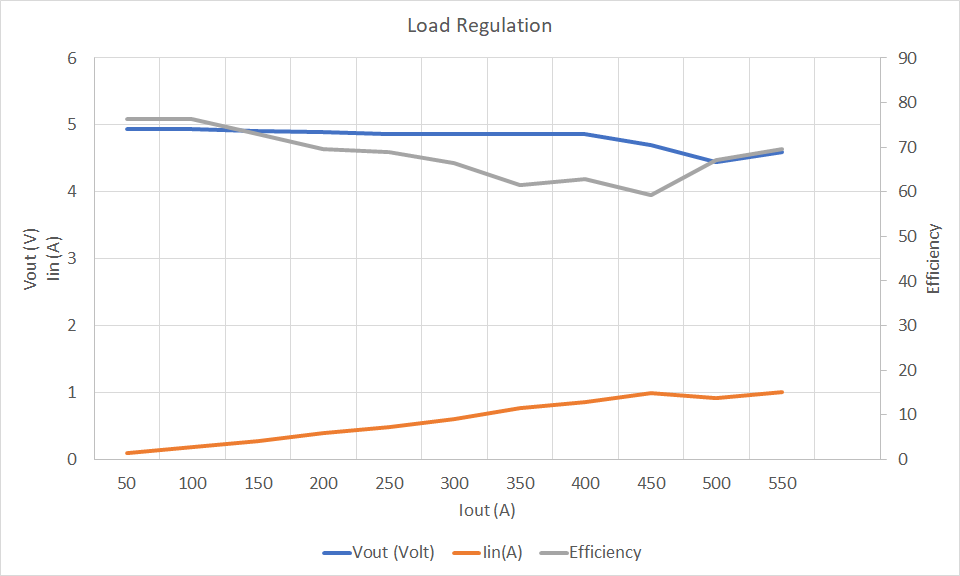
\includegraphics[width=\columnwidth]{IMGS/Boost load regulation at 3.6V Vin.png}
	\caption{Boost load regulation at 3.6V Vin}
	\label{fig:arch}
\end{figure}
\begin{table}[H]
\centering
\begin{tabular}{|l|l|l|l|}
\hline
Iout (mA) & Vout (Volt) & Iin(A) & Efficiency \\ \hline
50        & 4.94        & 0.07   & 84.01361   \\ \hline
100       & 4.93        & 0.15   & 78.25397   \\ \hline
150       & 4.9         & 0.2    & 87.5       \\ \hline
200       & 4.87        & 0.31   & 74.80799   \\ \hline
250       & 4.87        & 0.39   & 74.32845   \\ \hline
300       & 4.86        & 0.47   & 73.86018   \\ \hline
350       & 4.86        & 0.57   & 71.05263   \\ \hline
400       & 4.86        & 0.66   & 70.12987   \\ \hline
450       & 4.85        & 0.76   & 68.37406   \\ \hline
500       & 4.84        & 0.87   & 66.22879   \\ \hline
550       & 4.81        & 0.96   & 65.6126    \\ \hline
600       & 4.76        & 1.07   & 63.5514    \\ \hline
650       & 4.62        & 1.13   & 63.27434   \\ \hline
700       & 4.45        & 1.19   & 62.32493   \\ \hline
750       & 4.38        & 1.21   & 64.63991   \\ \hline
800       & 4.1         & 1.26   & 61.98035   \\ \hline
\end{tabular}
\caption{Boost load regulation at 4.2V Vin}
\label{table:4}
\end{table}
\\ 
\begin{figure}[H]
	\centering
	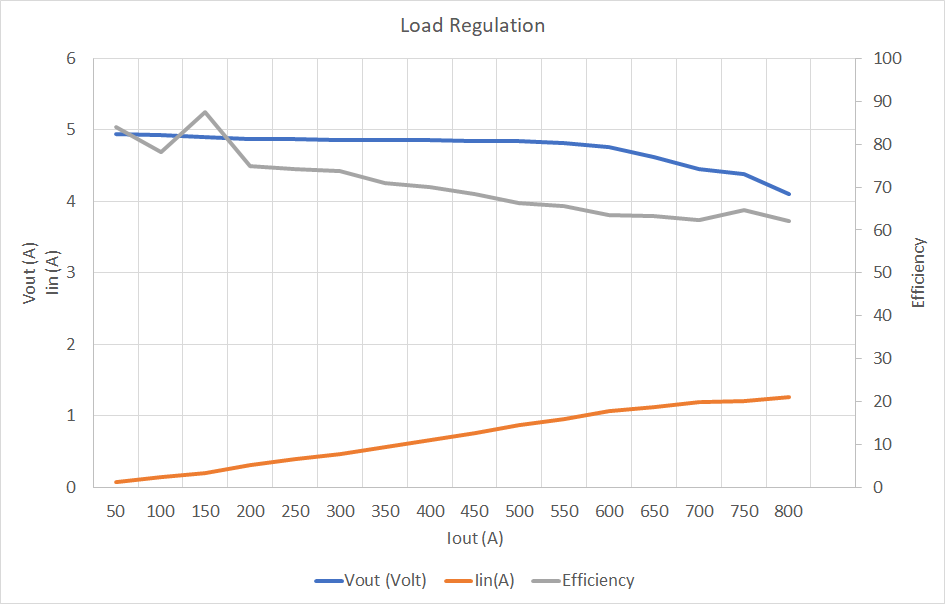
\includegraphics[width=0.9\columnwidth]{IMGS/Boost load regulation at 4.2V Vin.png}
	\caption{Boost load regulation at 4.2V Vin}
	\label{fig:arch}
\end{figure}
\begin{table}[H]
\centering
\begin{tabular}{|l|l|l|l|}
\hline
Iout (mA) & Vout (Volt) & Iin(A) & Efficiency \\ \hline
100       & 4.93        & 0.12   & 82.16667   \\ \hline
200       & 4.87        & 0.25   & 77.92      \\ \hline
300       & 4.86        & 0.39   & 74.76923   \\ \hline
400       & 4.84        & 0.54   & 71.7037    \\ \hline
500       & 5.02        & 0.66   & 76.06061   \\ \hline
600       & 5.02        & 0.85   & 70.87059   \\ \hline
700       & 5.02        & 1.01   & 69.58416   \\ \hline
800       & 5.02        & 1.19   & 67.4958    \\ \hline
\end{tabular}
\caption{Boost load regulation at 5.0V Vin}
\label{table:4}
\end{table}
\\
\begin{figure}[H]
	\centering
	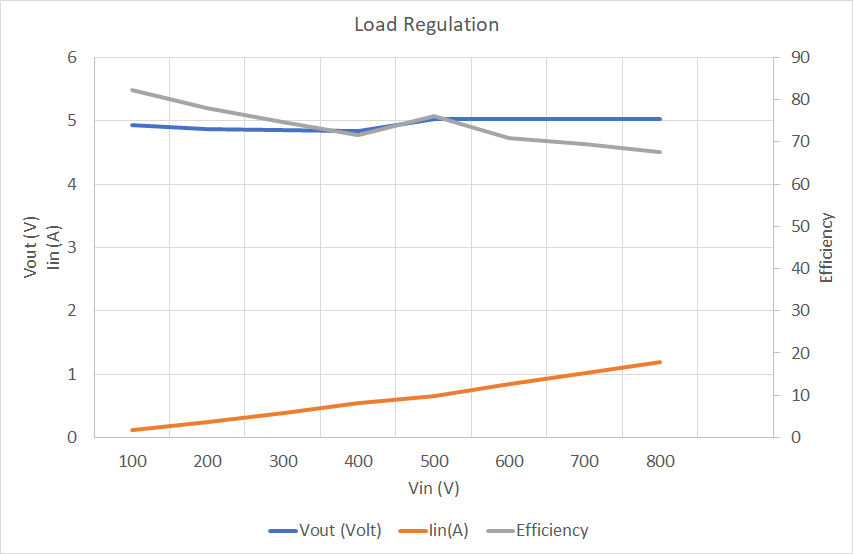
\includegraphics[width=\columnwidth]{IMGS/Boost load regulation at 5V Vin.png}
	\caption{Boost load regulation at 5.0V Vin}
	\label{fig:arch}
\end{figure}

\begin{table}[H]
\centering
\begin{tabular}{|l|l|l|l|}
\hline
Iout (mA) & Vout (Volt) & Iin (A) & Efficiency \\ \hline
50        & 3.32        & 0.06    & 76.85185   \\ \hline
100       & 3.28        & 0.11    & 82.82828   \\ \hline
150       & 3.28        & 0.16    & 85.41667   \\ \hline
200       & 3.27        & 0.21    & 86.50794   \\ \hline
250       & 3.2         & 0.27    & 82.30453   \\ \hline
300       & 3.22        & 0.32    & 83.85417   \\ \hline
350       & 3.21        & 0.38    & 82.12719   \\ \hline
\end{tabular}
\caption{Buck load regulation at 3.6V input}
\label{table:4}
\end{table}
\\
\begin{figure}[H]
	\centering
	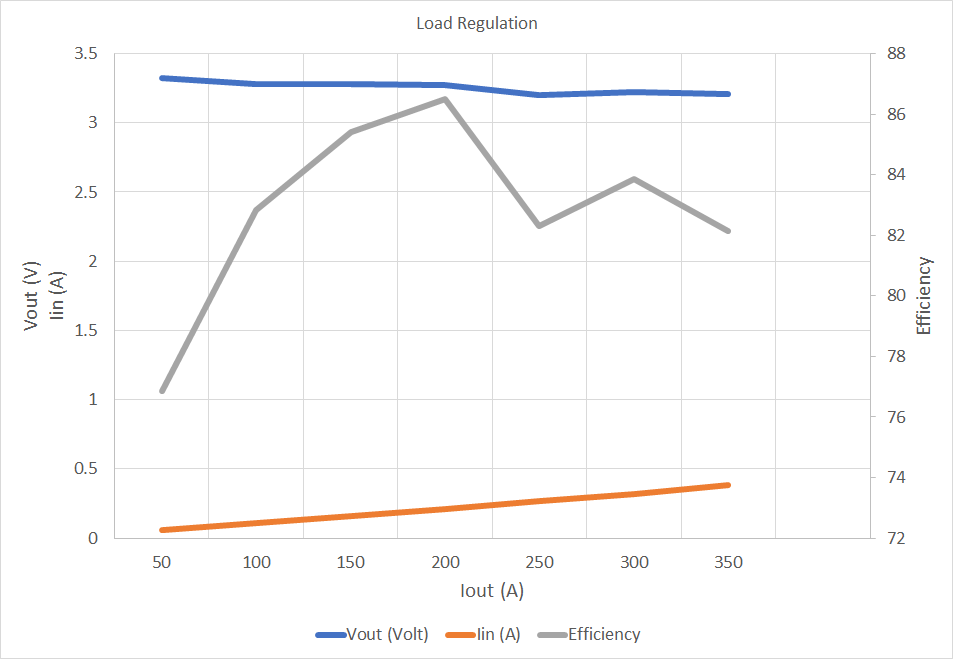
\includegraphics[width=\columnwidth]{IMGS/Buck load regulation at 3.6V input.png}
	\caption{ Buck load regulation at 3.6V input}
	\label{fig:arch}
\end{figure}
\\
\begin{table}[H]
\centering
\begin{tabular}{|l|l|l|l|}
\hline
Iout (mA) & Vout (Volt) & Iin (A) & Efficiency \\ \hline
50        & 3.24        & 0.04    & 84.375     \\ \hline
100       & 3.23        & 0.08    & 84.11458   \\ \hline
150       & 3.23        & 0.12    & 84.11458   \\ \hline
200       & 3.21        & 0.16    & 83.59375   \\ \hline
250       & 3.21        & 0.21    & 79.6131    \\ \hline
300       & 3.22        & 0.25    & 80.5       \\ \hline
350       & 3.18        & 0.27    & 85.87963   \\ \hline
\end{tabular}
\caption{Buck load regulation at 4.8V input}
\label{table:4}
\end{table}
\\
\begin{figure}[H]
	\centering
	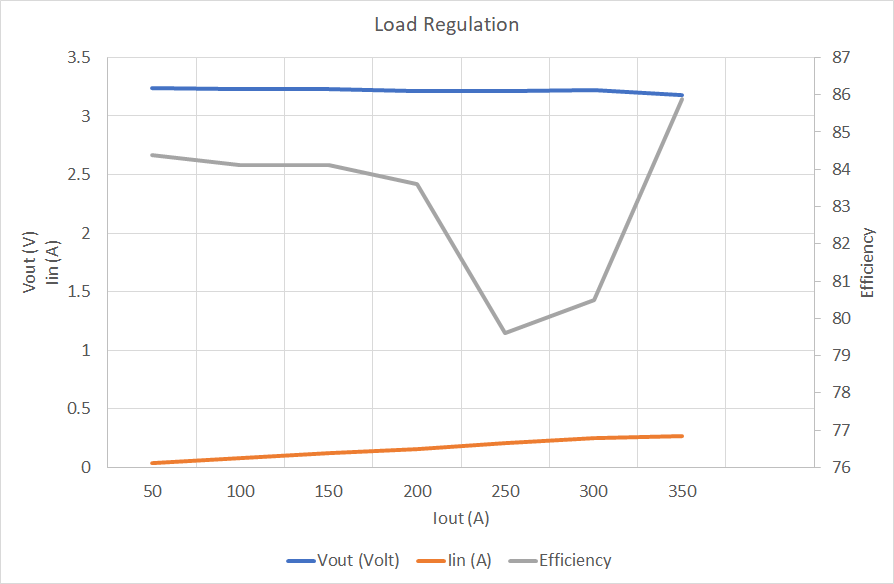
\includegraphics[width=\columnwidth]{IMGS/Buck load regulation at 4.8V input.png}
	\caption{Buck load regulation at 4.8V input}
	\label{fig:arch}
\end{figure}
\begin{table}[H]
\centering
\begin{tabular}{|l|l|l|l|}
\hline
Iout (mA) & Vout (Volt) & Iin (A) & Efficiency \\ \hline
50        & 3.3         & 0.03    & 91.66667   \\ \hline
100       & 3.21        & 0.06    & 89.16667   \\ \hline
150       & 3.26        & 0.1     & 81.5       \\ \hline
200       & 3.21        & 0.13    & 82.30769   \\ \hline
250       & 3.22        & 0.15    & 89.44444   \\ \hline
\end{tabular}
\caption{Buck load regulation at 6V input}
\label{table:4}
\end{table}
\\
\begin{figure}[H]
	\centering
	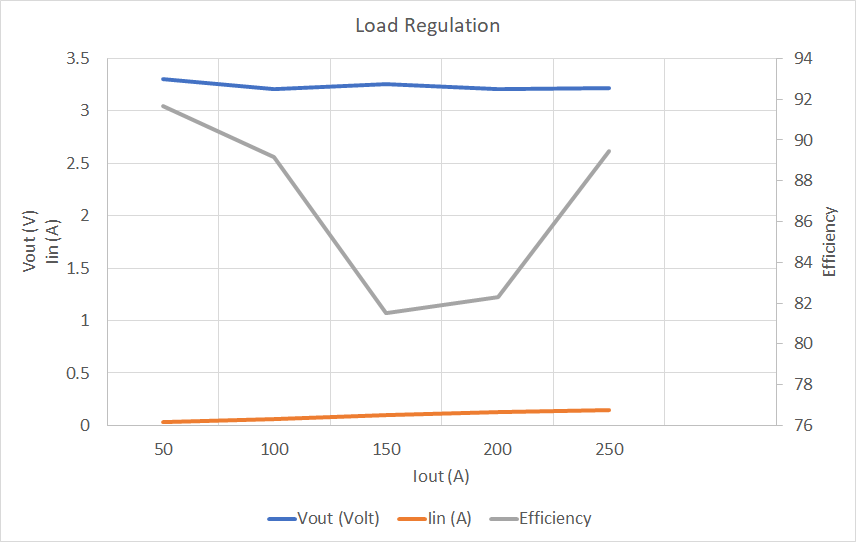
\includegraphics[width=\columnwidth]{IMGS/Buck load regulation at 6V input.png}
	\caption{Buck load regulation at 6V input}
	\label{fig:arch}
\end{figure}

% \subsection{Output transient response deviation and time}

%  This test determines how well the output voltage responds to a sudden change in output current. The measurement includes the maximum output voltage deviation and the time it takes for the voltage to recover to its regulated output nominal voltage tolerance.
% \\ \\
% For this test, a dc electronic load is set for a minimum and maximum current and then set for the slew rate for the rising and falling edge of the current transition. The frequency and duty cycle can also be set for the pulsed current.
% \\ \\
% \subsection{Output ripple and noise voltage} 

% The output ripple and PARD reflects the output voltage of the DC/DC converter and its ability to filter out ripple and noise. Various topologies used in DC/DC converters have different internal switching frequencies which are reflected in the output ripple frequency. For example, internal chopper circuit transients can generate higher frequency noise. The output noise and ripple are measured using an oscilloscope. To avoid erroneous noise, it is important to minimize the length of the ground wire on the voltage probe.
% \\ \\
\subsection{Output over-current protection}

The output over-current protection is intended to protect the DC/DC converter and the device it powers when the load exceeds the converter’s maximum rated current. There are different methods used in over-current protection. But the typical approaches are fold-back current limit and pulsing current-limit. The latter is generally referred to as hiccup-mode current limit.
\\ \\
Here are the differences between the two methods: In fold-back current limiting, the output voltage begins to drop and limits the output current supplied to the load as the load current rises above the current-limit set point. In hiccup current limiting, the output turns off when the output current exceeds the rated current limit point. It eventually turns back on. If the load continues to exceed the current-limit set-point, the output will continue turning on and off, hence the hiccup-mode name.
\\ \\
\subsection{Output over-voltage protection} 

Most DC/DC converters have a built-in protection circuit that will shut off the output of the device when the output voltage is detected to be over the maximum limit. This facility is referred to as over-voltage protection (OVP). This protects the DC/DC converter from external excessive voltage applied to the converter output. If the DC/DC converter has an adjustable output (trimmed or programmable output voltage), it may be possible to increase the output voltage until the OVP point is exceeded and the protection circuit activates.
\\ \\
If the DC/DC converter does not have an adjustable output, an external voltage source can be applied across the output terminal, increased to the OVP trip point, then removed to see if the output has triggered and turned off.
\\ \\
DC/DC converters having an OVP fault signal can use it to determine if the output detected the OVP and, if so, shut off the output. The output voltage is monitored to determine when the OVP happened and then compared to the OVP specified limits.
\\ \\
% \subsection{Output operating temperature and over-temperature protection} 

% DC/DC converters have an operating temperature range, and many have an over-temperature protection (OTP) circuit that will turn off the output if temperature gets sufficiently high. For this test, a thermal chamber can raise and lower the DC/DC converter temperature to simulate the operating temperature range.
% \\ \\
% Thermocouples and thermal probes or infrared thermal measurement devices can measure the temperatures on the body of the DC/DC converter. During the operating temperature test, the DC/DC converter is loaded to its maximum rating for current and power. Meanwhile, the output voltage is monitored to verify it stays within specified limits.
% \\ \\
% During the test, the device temperature is recorded while monitoring the output voltage until the OTP circuit triggers and the output shuts off. The unit is then allowed to cool and input voltage is toggled off and on to verify the DC/DC converter recovers from the OTP.
% \\ \\
\subsection{Efficiency} 

Efficiency determines the internal power dissipated by the DC/DC converter and how efficiently input power transfers to the converter output. This test usually takes place at the nominal input voltage and with the output load set to nominal or maximum specified ratings. The input voltage, current, and power is measured while the same parameters are measured on the output. Efficiency percentage $E_{p}$ comes from the equation:
\\ \\
\hspace*{5cm}$E_{p}$ = $\left | \frac{V_{out}-I_{out}}{V_{in}-I_{in}} \right | \times 100$
\\ \\
where:
Vout and Iout = converter output voltage and current;
Vin and Iin = converter input voltage and current.
\\ \\
This test can also capture the efficiency at various power levels. It’s common to plot the data to show efficiency versus output-current.

\section{Battery Charger Testing}
 The battery charger IC selected was BQ25302 which is a Li-ion constant current - constant voltage (CCCV) charger. With the constant current function pumping current into the battery, its voltage obviously rises. And as soon as it reaches the set charging voltage of the IC the current
falls underneath the constant current limit and thus it enters the constant voltage mode at which point the battery charges up to its max capacity where almost no current is flowing any more. This method is used to prevent overcharging of batteries.

In this circuit, the charging voltage was set at 4.2V as per the data-sheet of the battery. From fig. \ref{fig:cccv}, it is clear that the battery charges in constant current mode and its voltage rises to approximately 4.2V. Then the charger switches to constant voltage mode and the charging current reduces to zero eventually.

\begin{figure}[H]
	\centering
	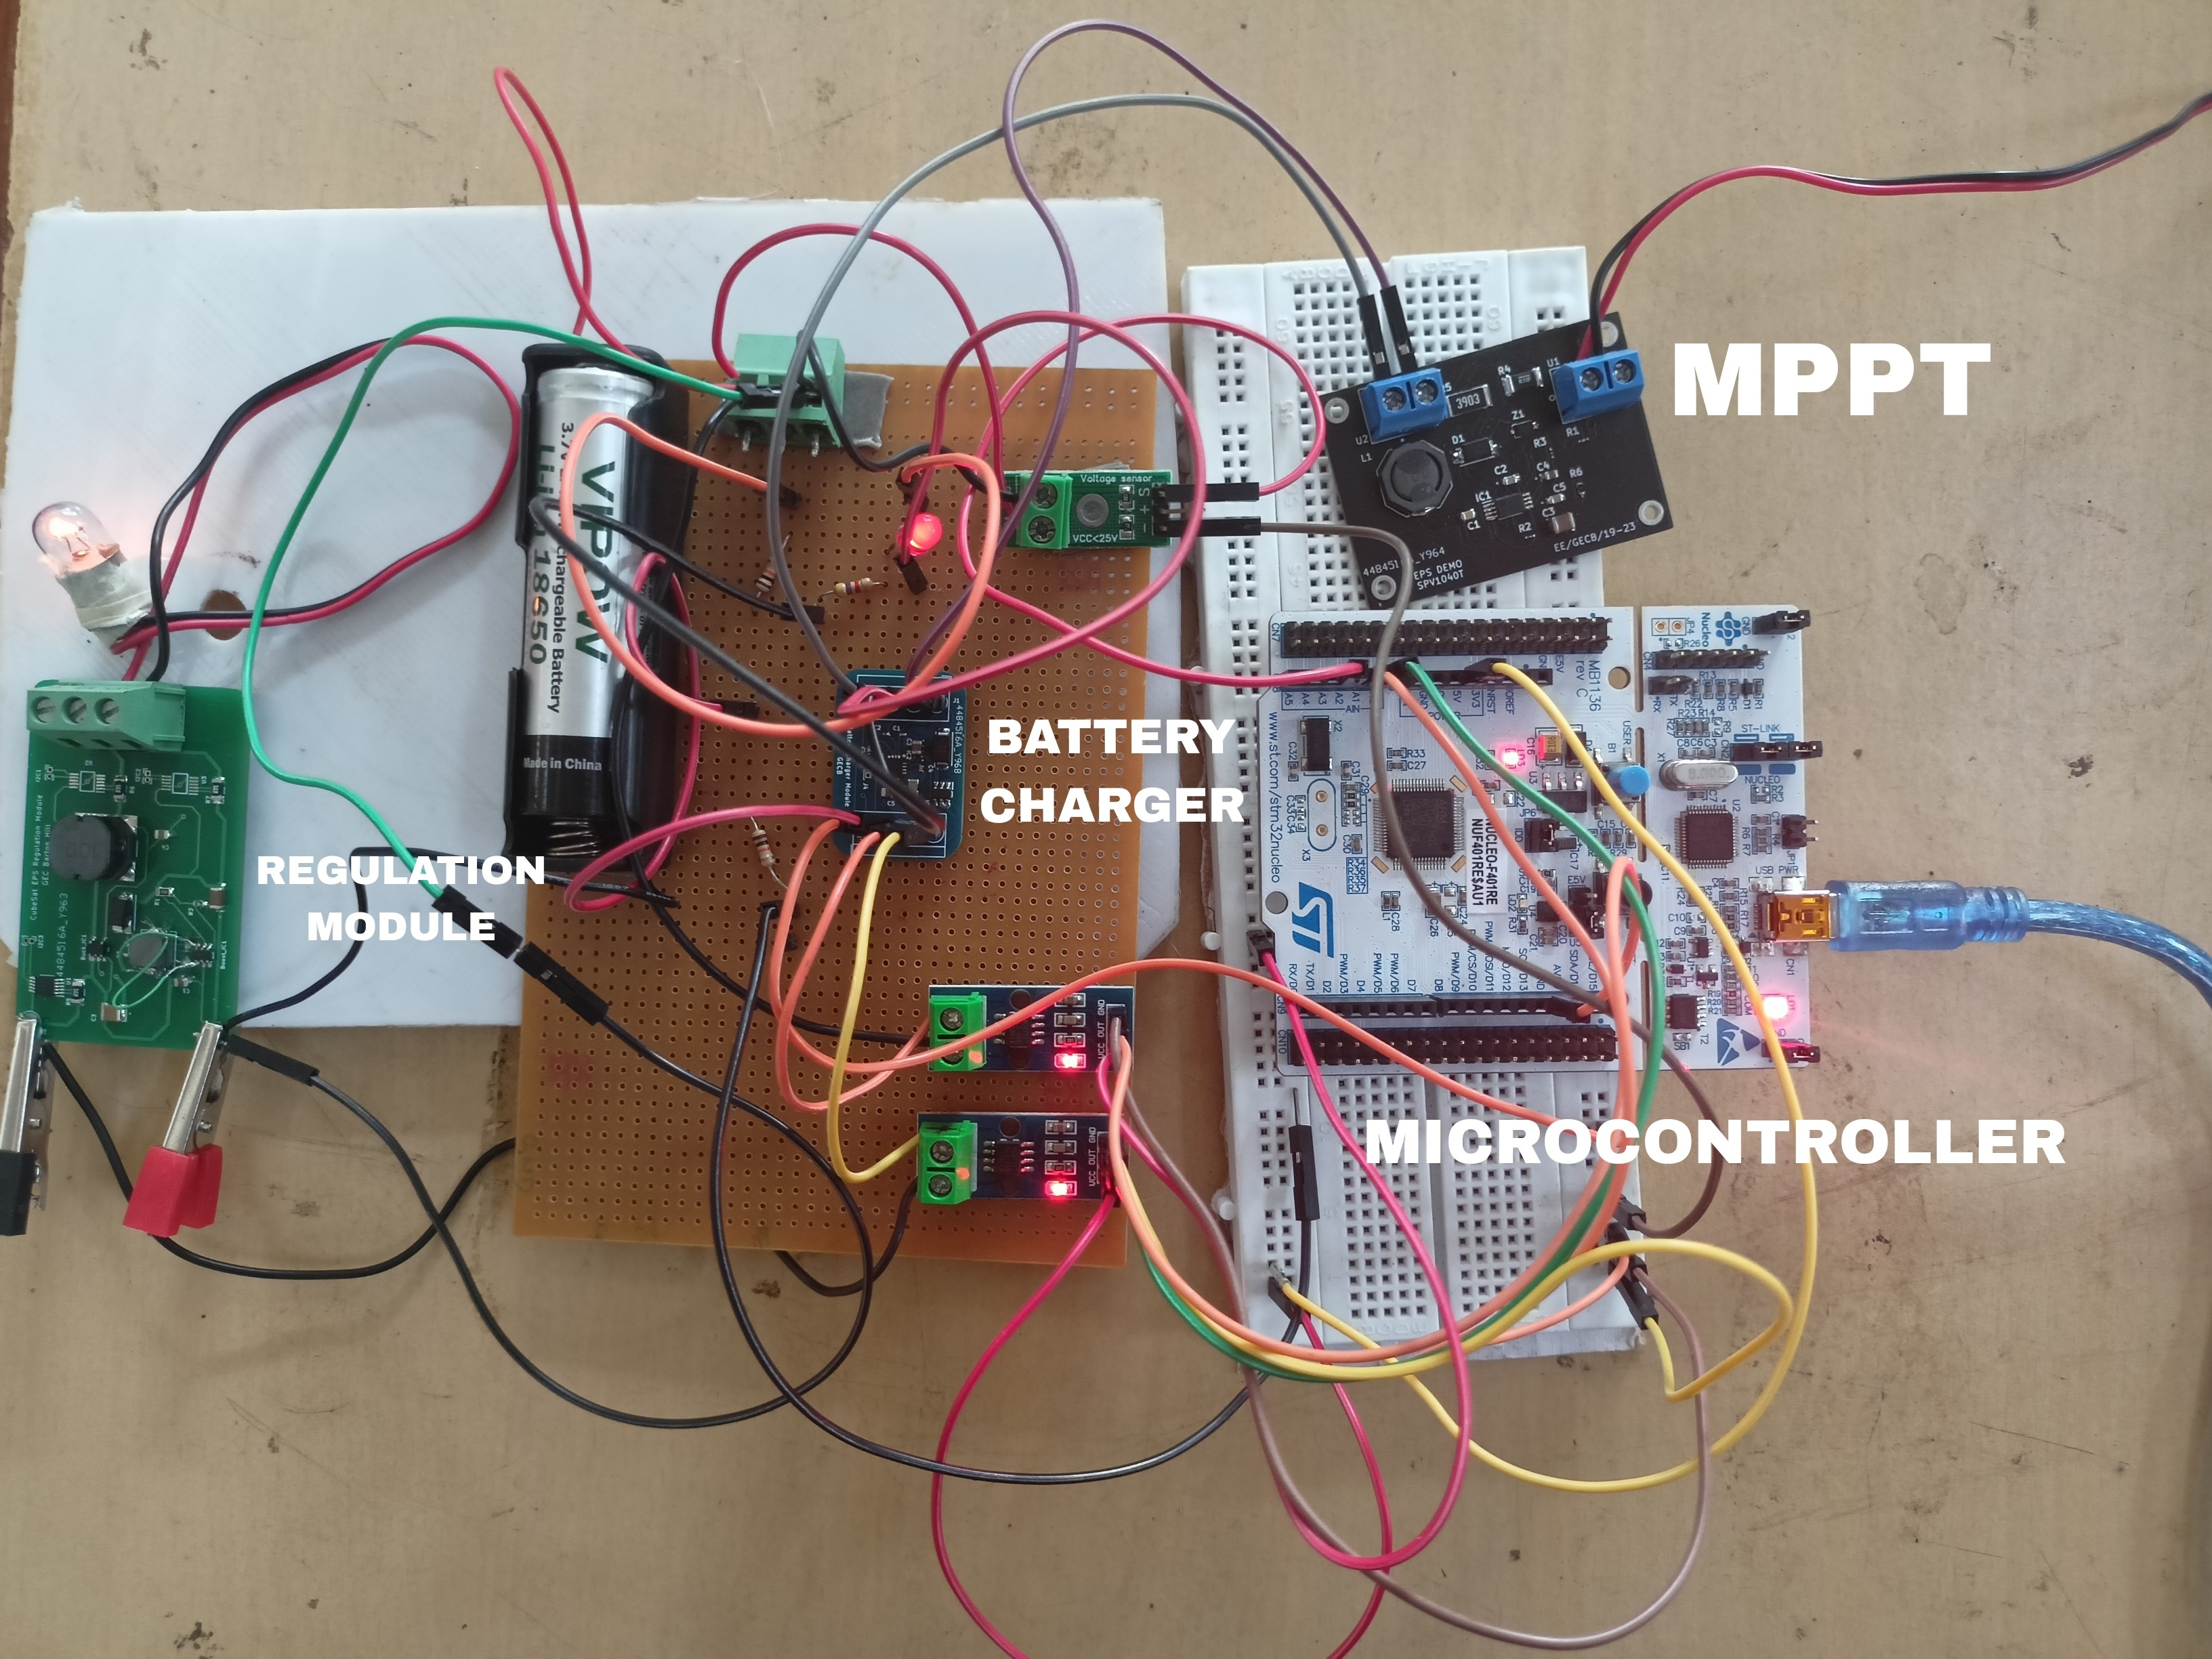
\includegraphics[width=0.72\columnwidth]{IMGS/TestSetupPics/Bat_cha_test.jpg}
	\caption{Battery charger test setup}
	\label{fig:arch}
\end{figure}

\begin{figure}[H]
	\centering
	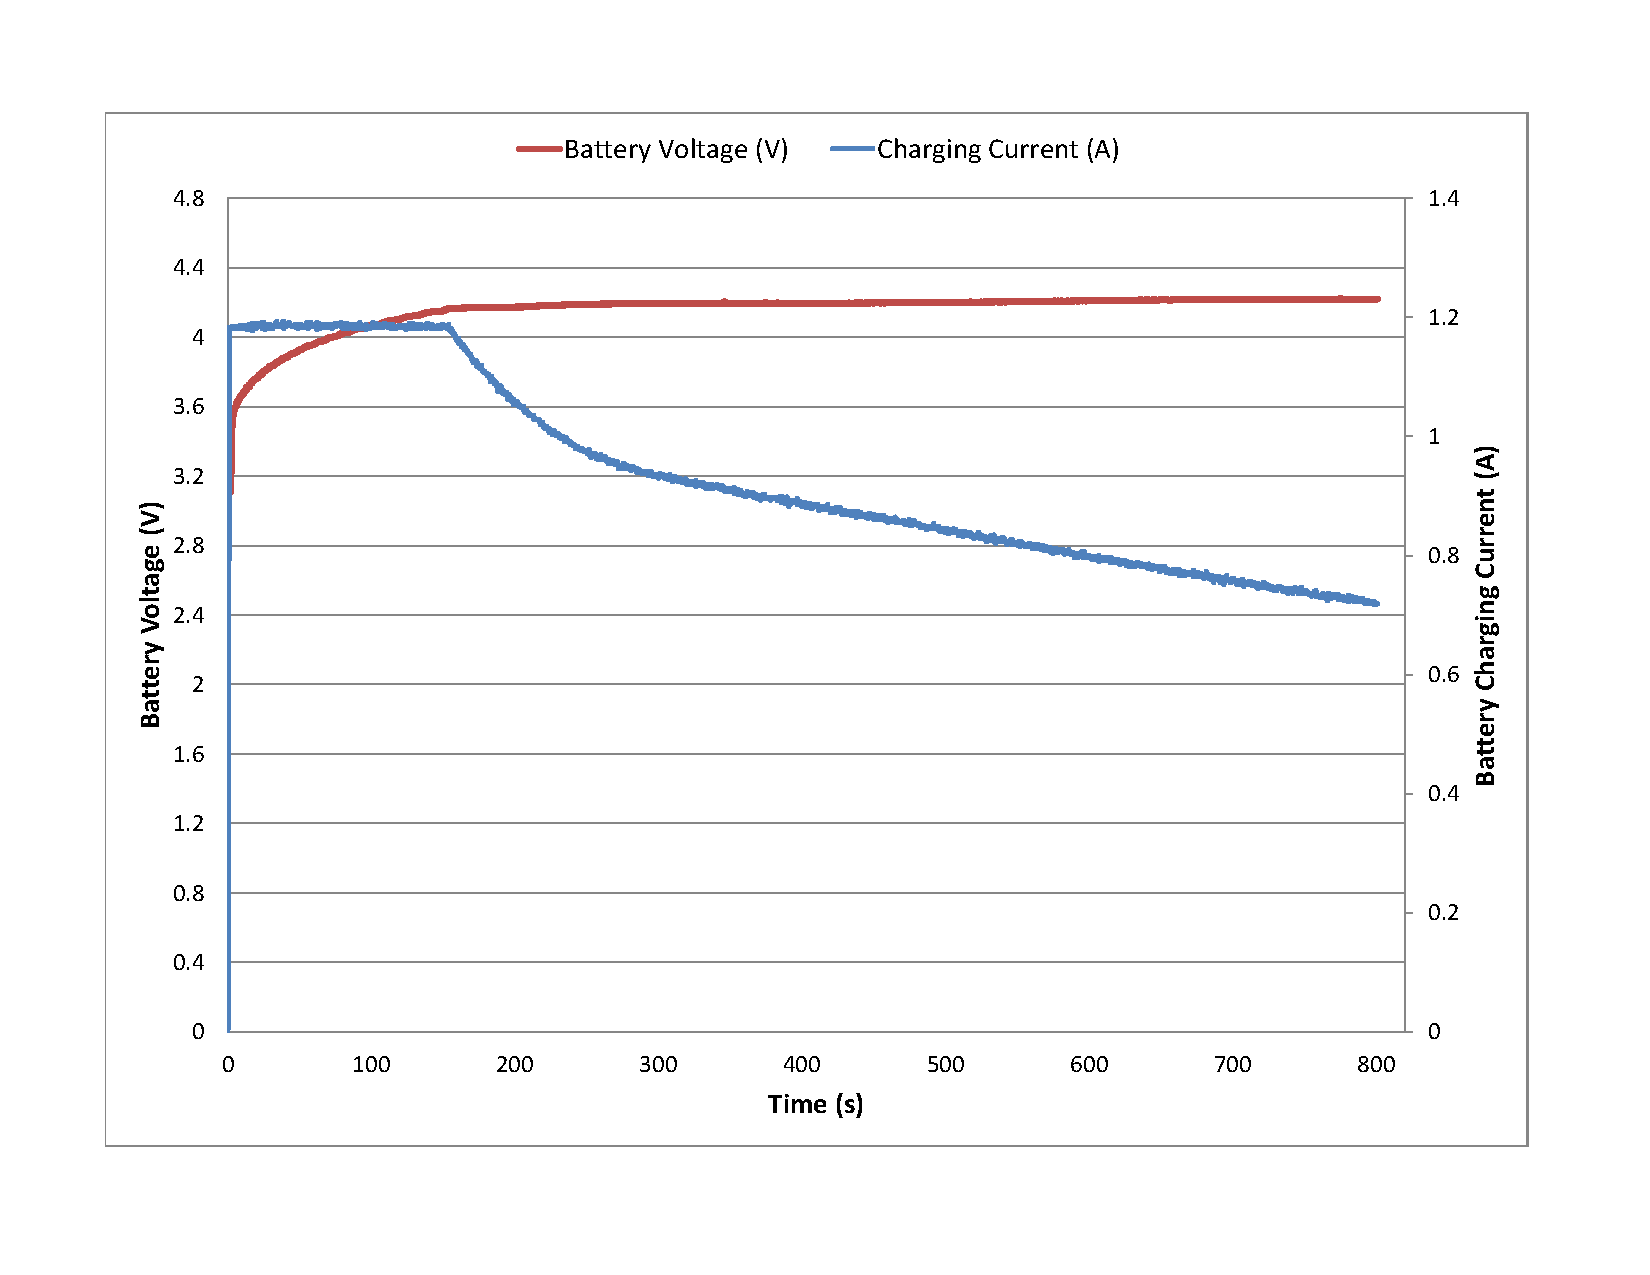
\includegraphics[width=0.9\columnwidth]{IMGS/Battery CC CV.pdf}
	\caption{Constant current and constant voltage charging}
	\label{fig:cccv}
\end{figure}

\begin{figure}[H]
	\centering
	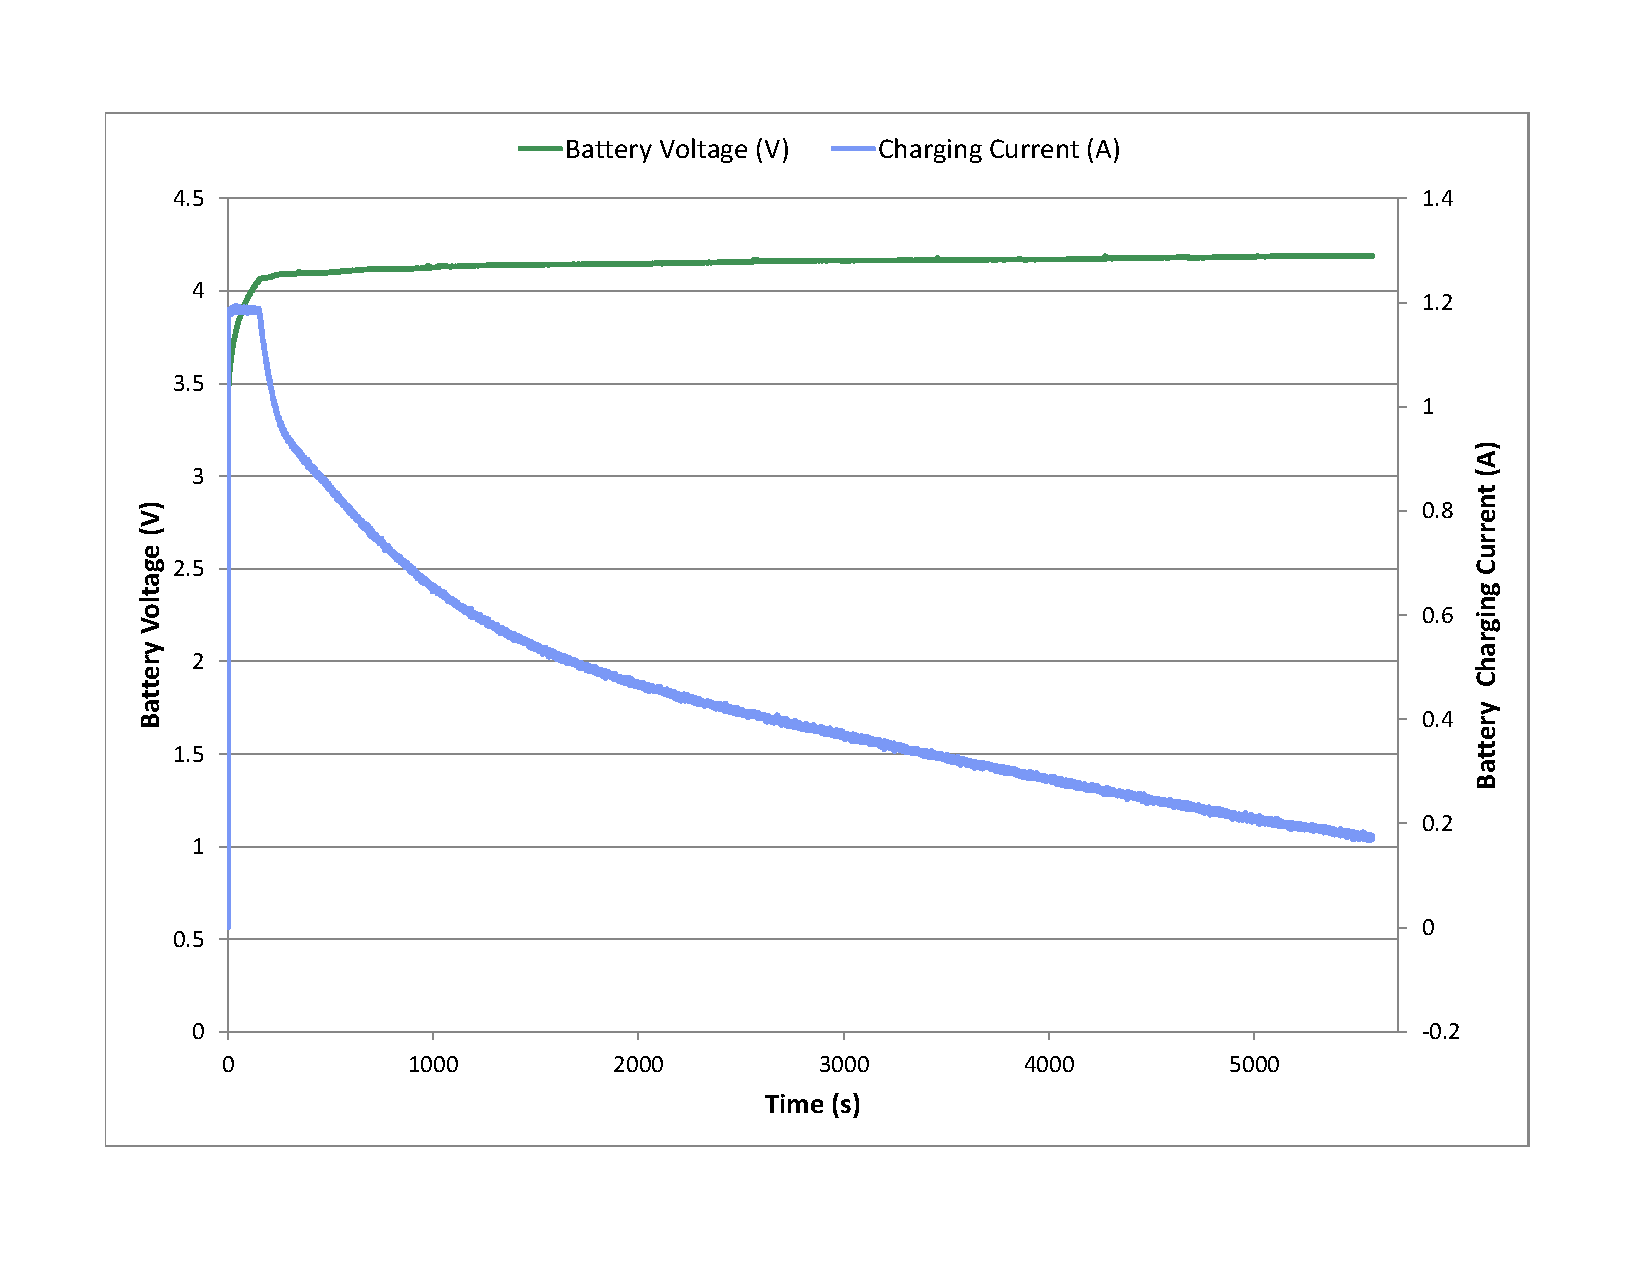
\includegraphics[width=\columnwidth]{IMGS/Battery Charge Cycle.pdf}
	\caption{Variation of charging voltage and current while charging the 18650 Li-Ion battery upto 100\%}
	\label{fig:chargin'}
\end{figure}
\section{MPPT Module Testing}

The demo board for MPPT is designed with SPV1040T IC, which has a lower cutoff voltage of 1V. Varying input voltages from solar panel is estimated to be between 2V-5V. The MPPT board will boost voltages in these range to 5V or larger and provide it to the battery charger. The basic working of the MPPT board is tested by providing an input voltage between 2V and 5V and measuring the output voltage, which will be 5V or more.

\begin{figure}[H]
	\centering
	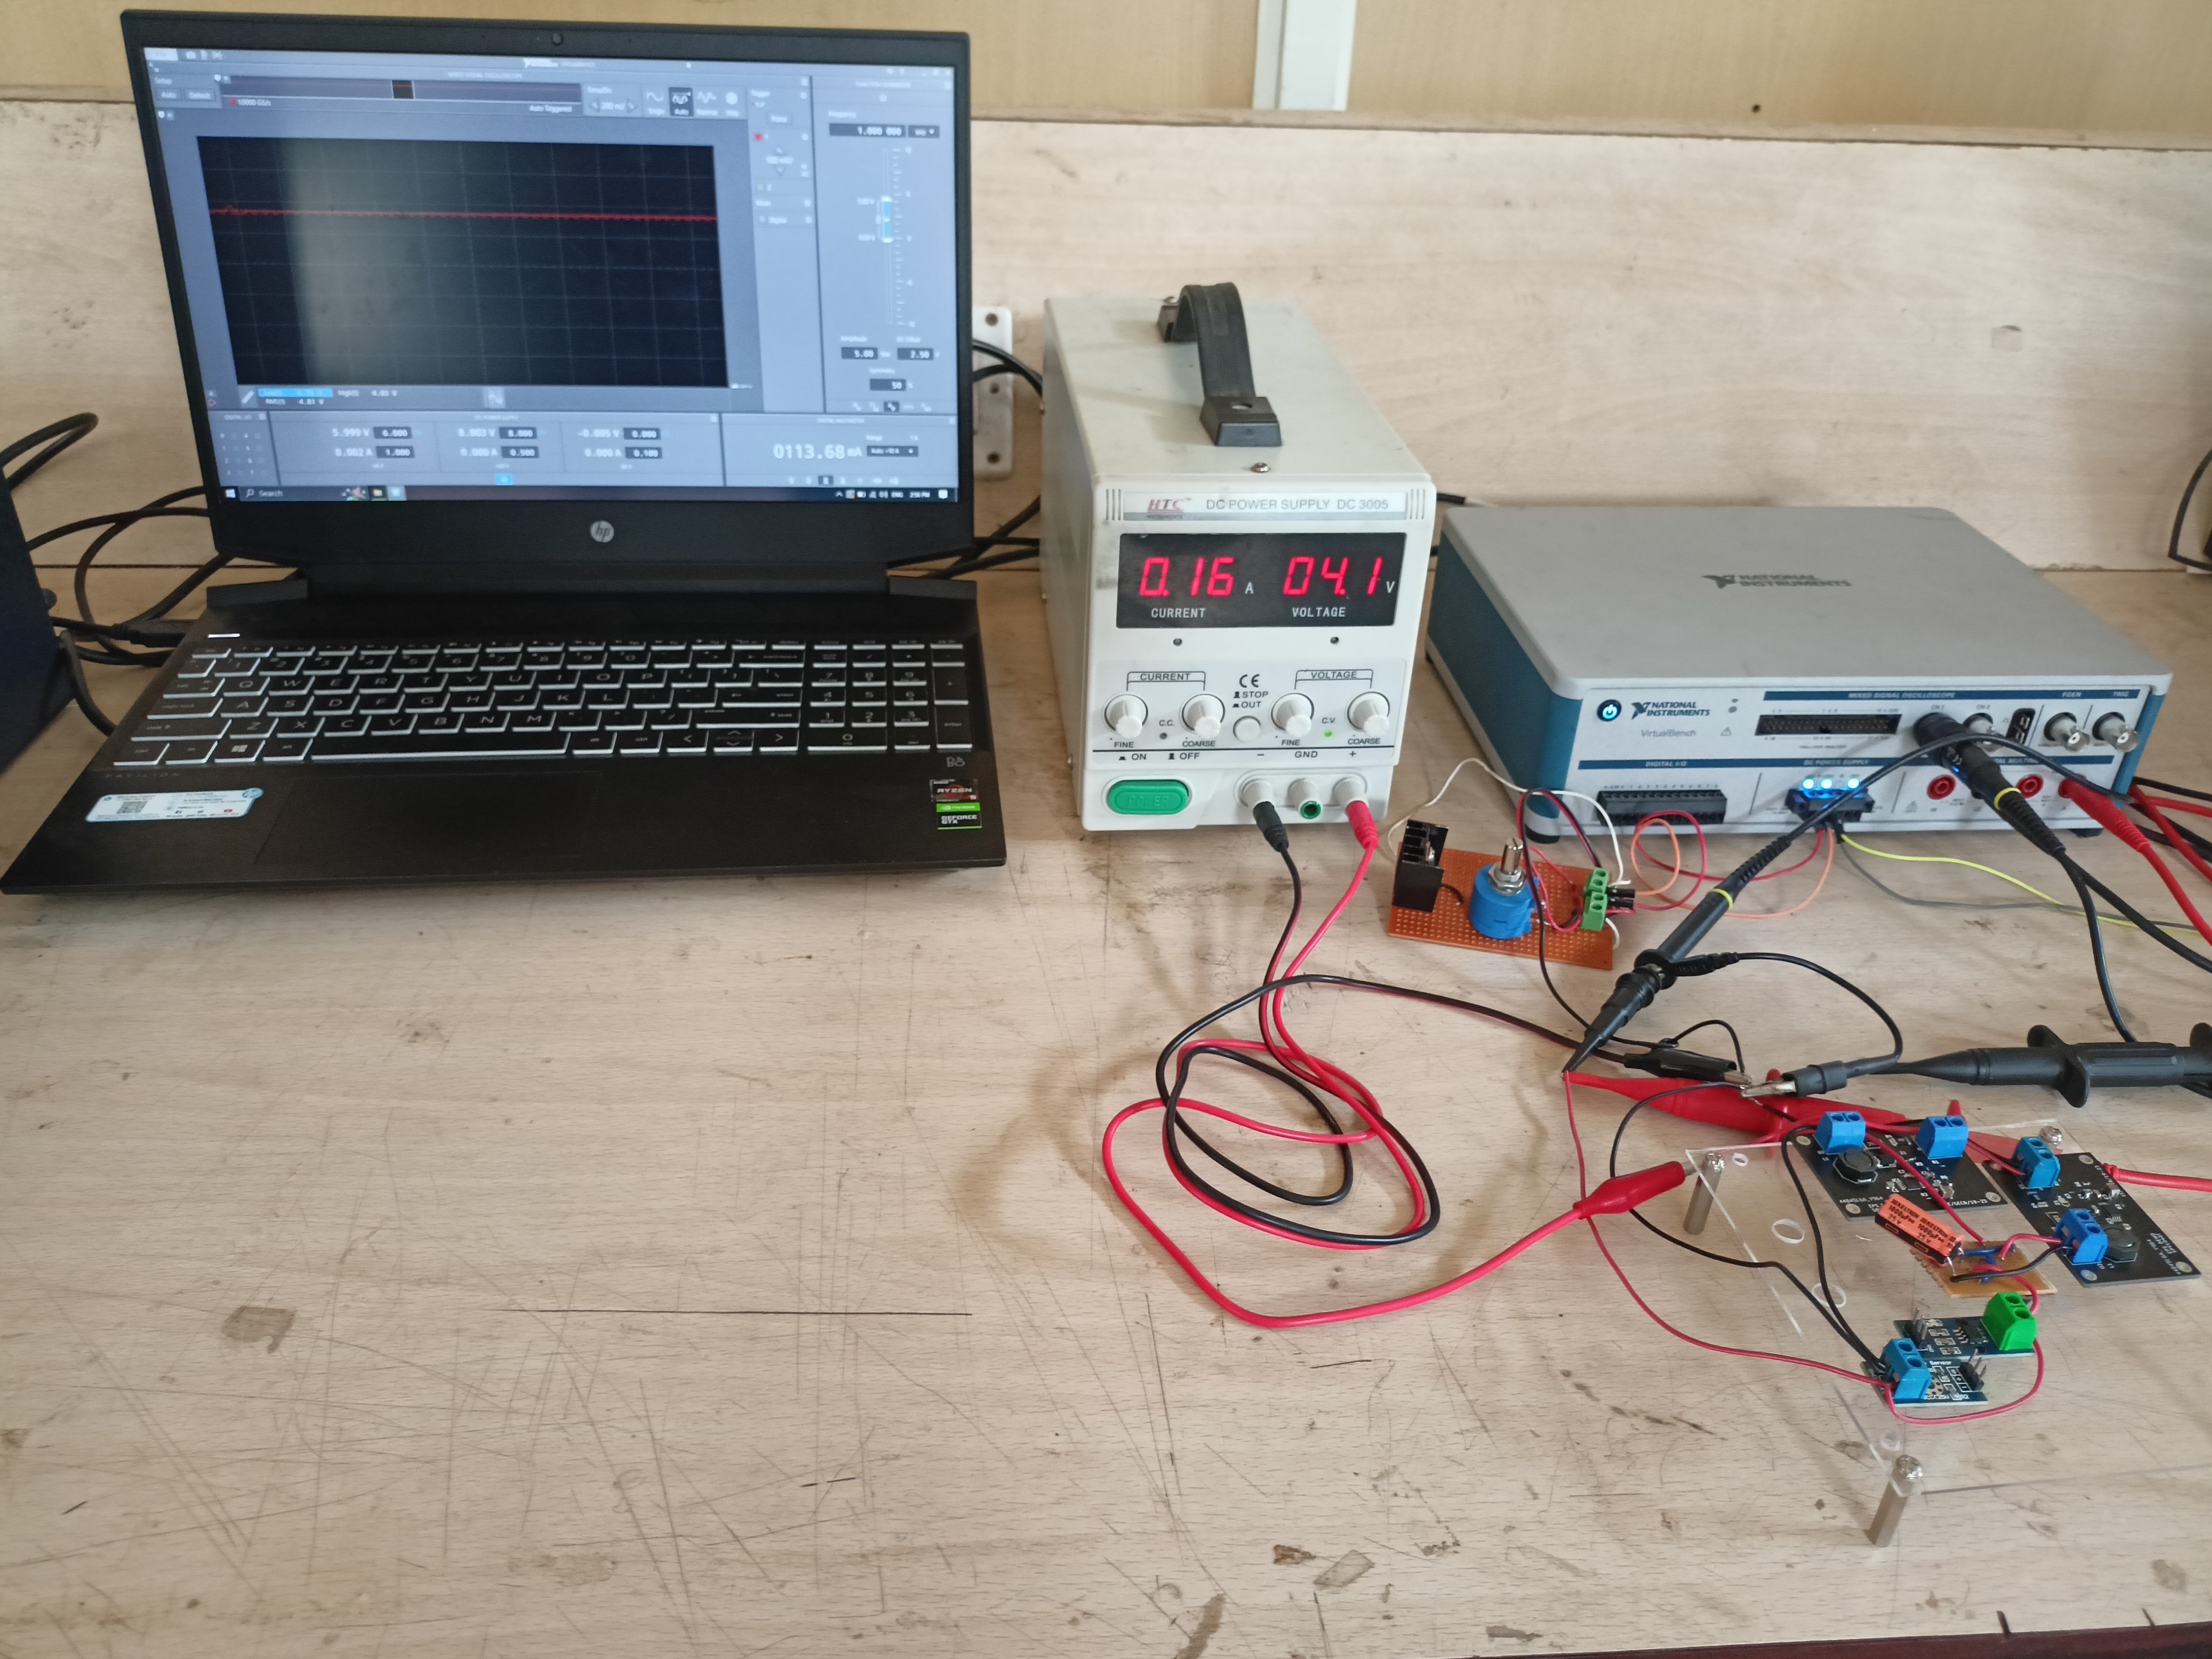
\includegraphics[width=0.7\columnwidth]{IMGS/TestSetupPics/TESTPIC_MPPT_MODULE.jpg}
	\caption{MPPT test setup}
	\label{fig:arch}
\end{figure}

\begin{figure}[H]
	\centering
	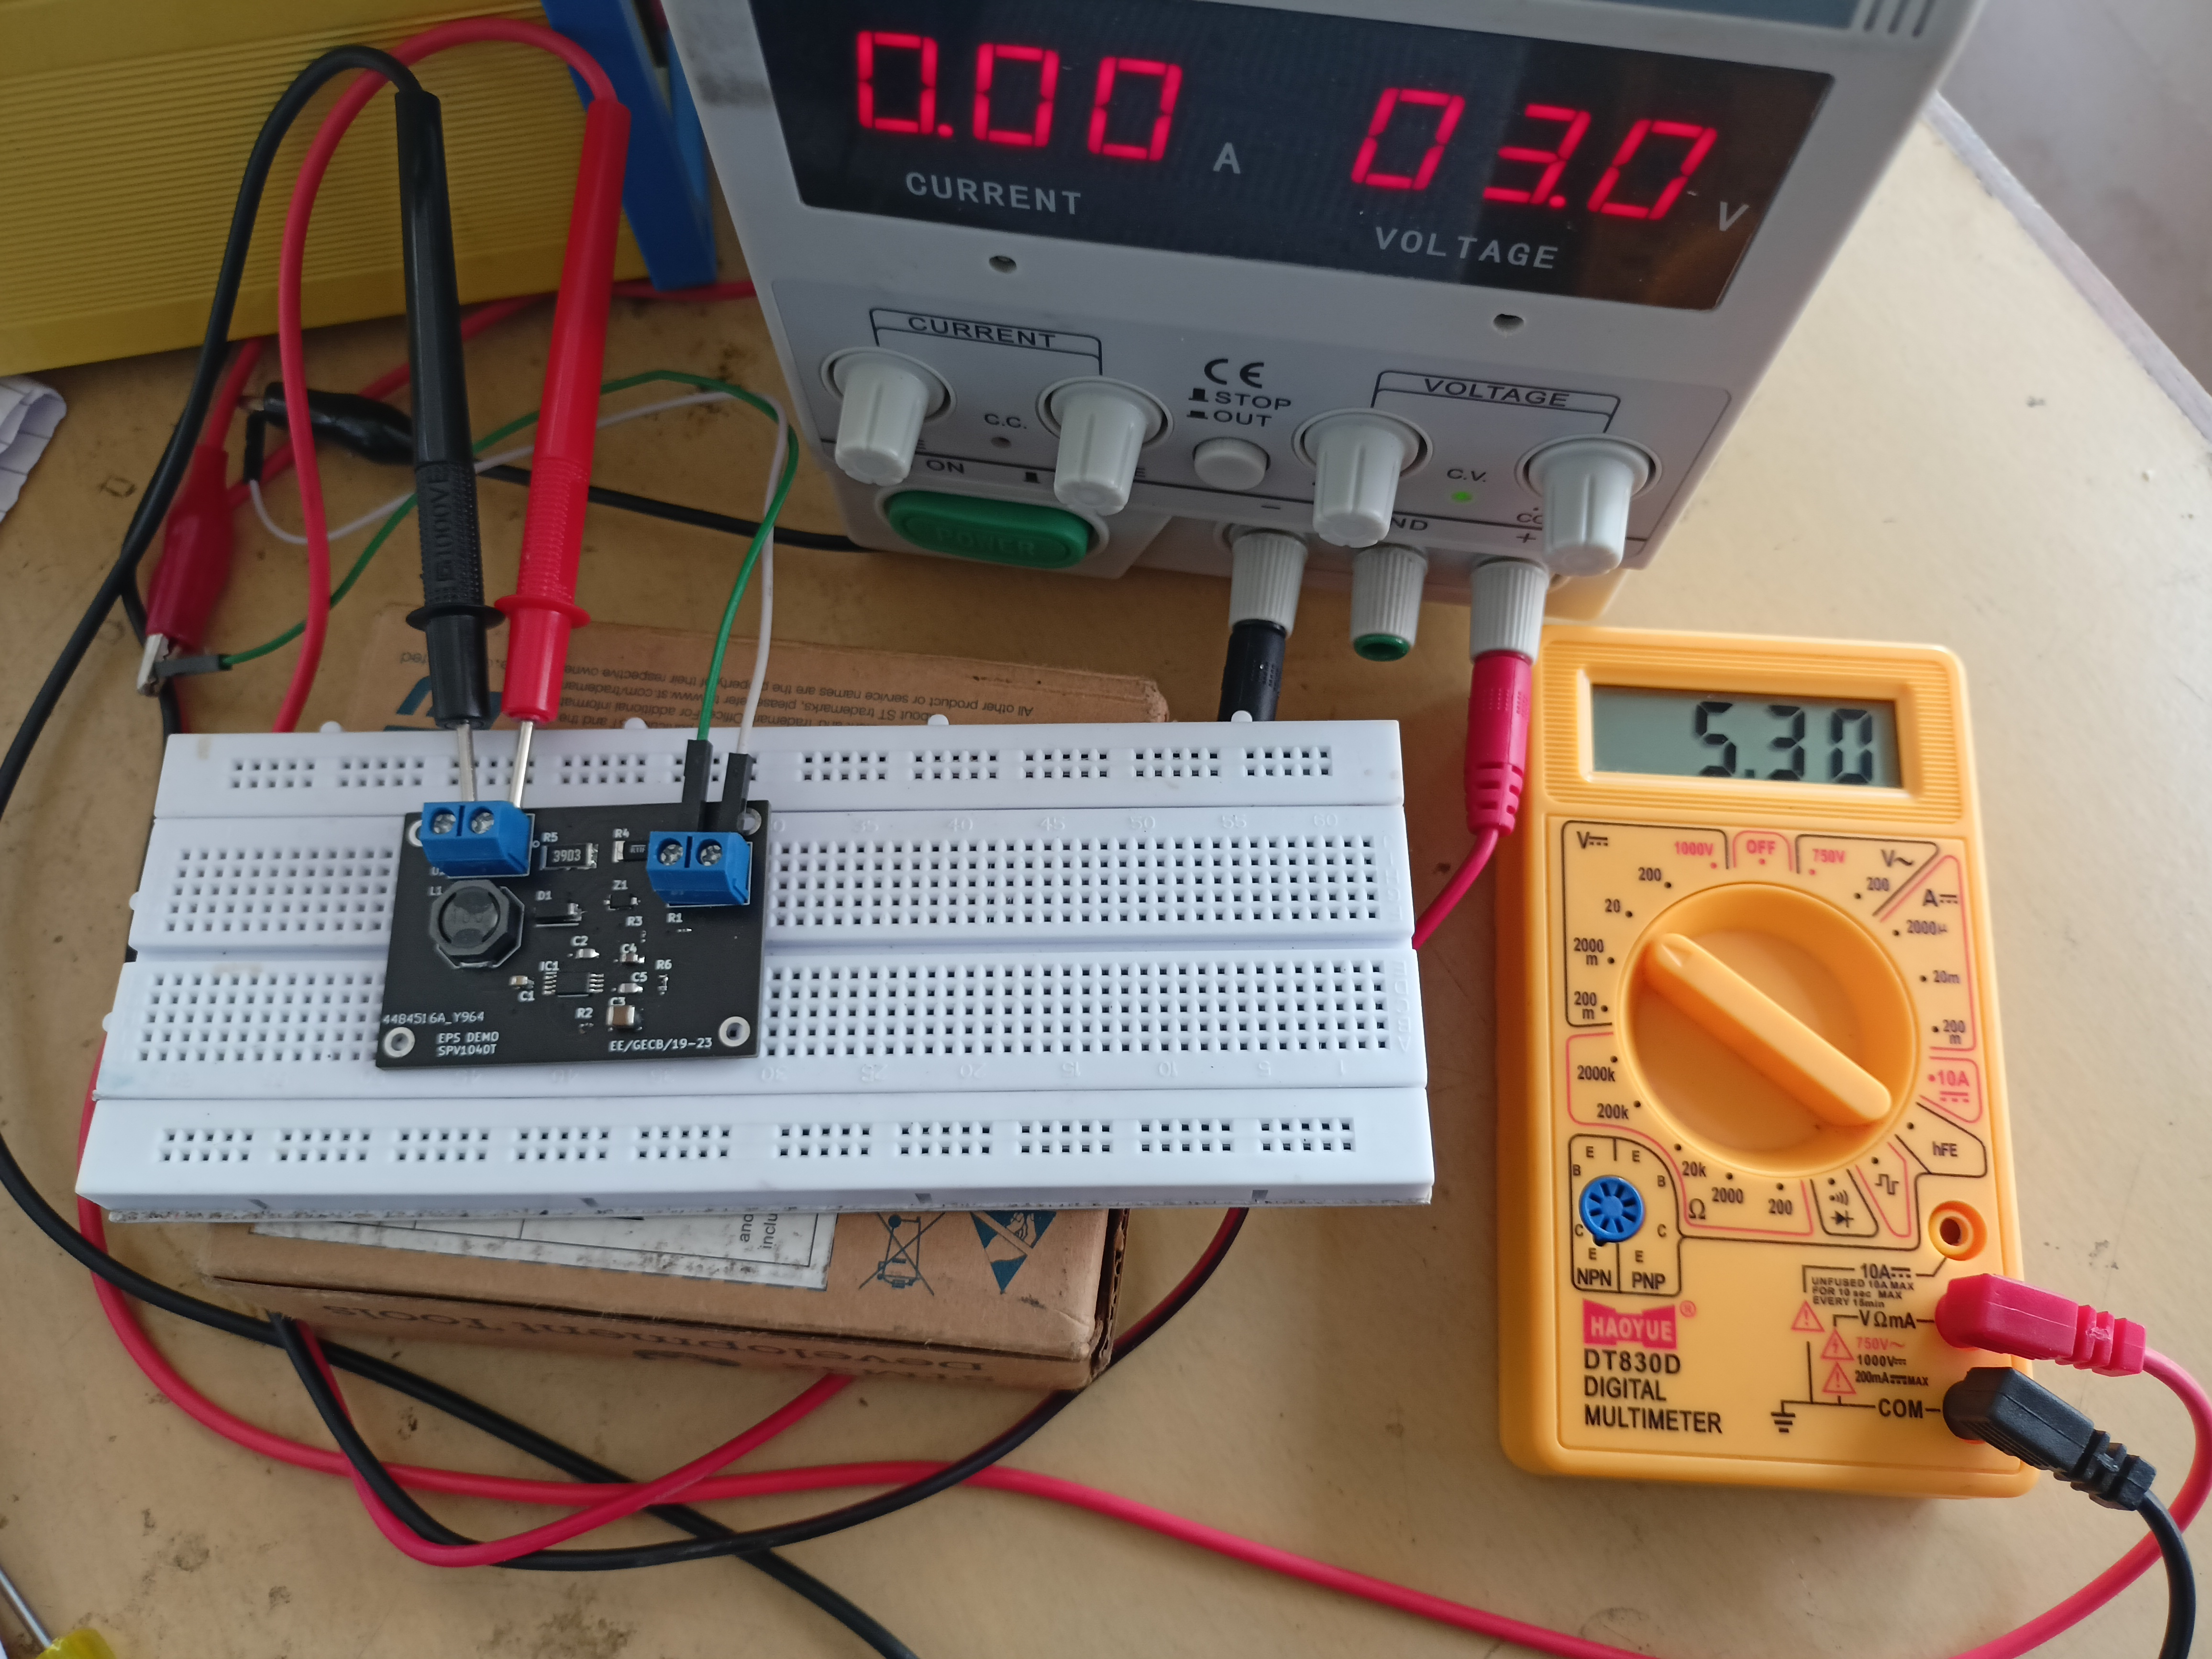
\includegraphics[width=0.7\columnwidth]{IMGS/TestSetupPics/MPPT_out.jpg}
	\caption{MPPT output voltage at no load}
	\label{fig:arch}
\end{figure}



\begin{table}[H]
\centering
\begin{tabular}{|l|l|l|l|}
\hline
Vin (Volt) & Iin (A) & Vout (Volt) & Efficiency \\ \hline
2          & 0.4     & 3.55        & 88.75      \\ \hline
2.5        & 0.35    & 3.9         & 89.14286   \\ \hline
3          & 0.29    & 4.19        & 96.32184   \\ \hline
3.3        & 0.28    & 4.38        & 94.80519   \\ \hline
3.6        & 0.27    & 4.55        & 93.6214    \\ \hline
4          & 0.26    & 4.8         & 92.30769   \\ \hline
4.2        & 0.25    & 4.95        & 94.28571   \\ \hline
4.6        & 0.24    & 5.11        & 92.57246   \\ \hline
\end{tabular}
\caption{MPPT output line regulation at half load (200mA)}
\label{table:4}
\end{table}	
\\
\begin{figure}[h]
	\centering
	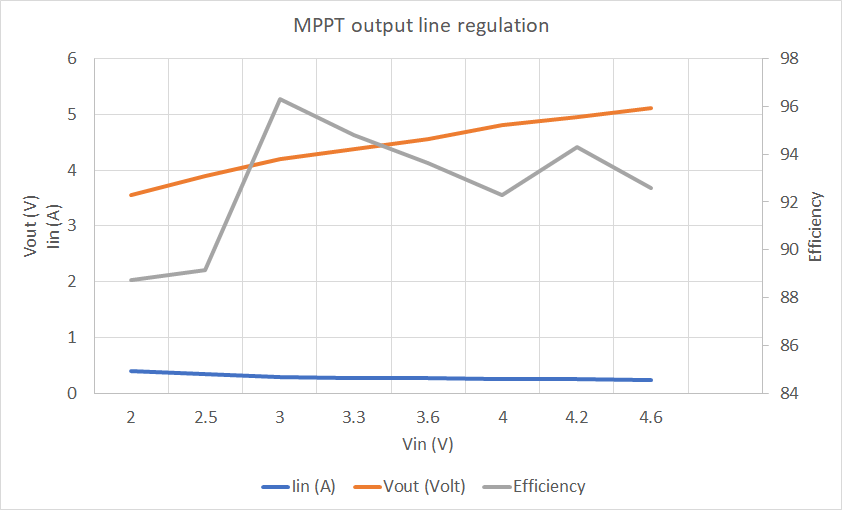
\includegraphics[width=\columnwidth]{IMGS/MPPT output line regulation at half load (200mA).png}
	\caption{MPPT output line regulation at half load (200mA)}
	\label{fig:arch}
\end{figure}

\begin{table}[H]
\centering
\begin{tabular}{|l|l|l|l|}
\hline
Vin (Volt) & Iin (A) & Vout (Volt) & Efficiency \\ \hline
2          & 0.39    & 1.88        & 98.82051   \\ \hline
2.5        & 0.43    & 2.48        & 94.58605   \\ \hline
3          & 0.45    & 3.02        & 91.71852   \\ \hline
3.3        & 0.46    & 3.39        & 91.56126   \\ \hline
3.6        & 0.44    & 3.78        & 97.84091   \\ \hline
4          & 0.45    & 4.2         & 95.66667   \\ \hline
4.2        & 0.45    & 4.41        & 95.66667   \\ \hline
4.6        & 0.49    & 5           & 90.94942   \\ \hline
\end{tabular}
\caption{MPPT output line regulation at full load (400mA)}
\label{table:4}
\end{table}

\begin{figure}[h]
	\centering
	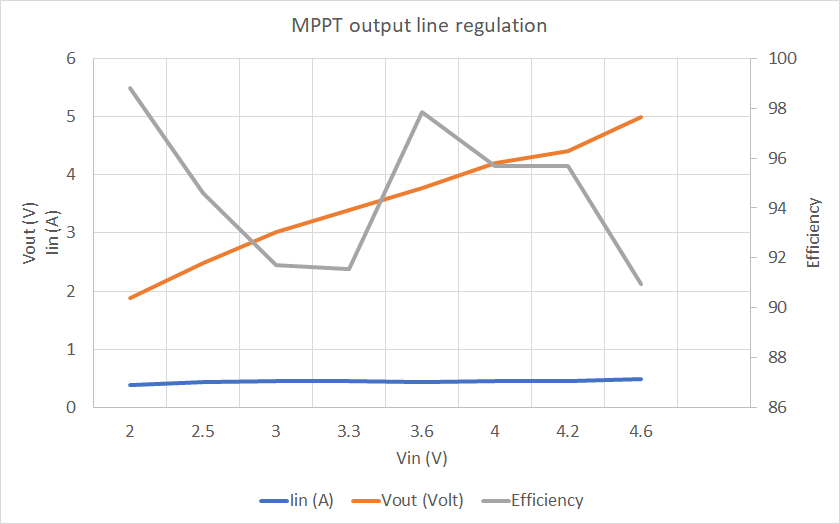
\includegraphics[width=\columnwidth]{IMGS/MPPT output line regulation at full load (400mA).png}
	\caption{MPPT output line regulation at full load (400mA)}
	\label{fig:arch}
\end{figure}









  

\chapter{Conclusion}

\begin{itemize}
	\item 			
\end{itemize}
%\section{Set Your Report Particulars}
%
%In order to setup report particulars, Afsin would configure the report as follows:
%
%\begin{verbatim}
%% Use one: Thesis/Capstone project report/Project report
%%\def\RoportType{Capstone project report\xspace} 
%\def\RoportType{Thesis\xspace}
%%\def\RoportType{Project report\xspace}
%
%\def\ReportTitle{Blockchain Based Food Distribution in the Planet
%Mars\xspace}
%\def\Supervisor{Dr. Mohammad Shahriar Rahman\xspace} 
%\def\SupervisorPosition{Associate Professor\xspace}
%%\def\reportSubmissionDate{\today}
%\def\reportSubmissionDate{February 02, 2029}
%\def\reportSubmissionTerm{Fall 2028}
%\end{verbatim}
%\section{Set Group Members Particulars}
%According to the description given in Sec \ref{sec:how}, Afsin would configure the group members particulars as follows:
%\begin{verbatim}
%\def\numberOfAuthors{1} % write 1, 2 or 3 (depends on your group)
%%
%\def\firstAuthor{Afsin Fairuz\xspace} 
%\def\firstAuthorID{243014007\xspace}
%\def\firstAuthorFatherName{Manzurul Haque\xspace}
%\def\firstAuthorMotherName{Mansura Akhter\xspace}
%\end{verbatim}
%
%\section{Changing Chapter Title}
%In order to create a new chapter or rewrite the chapter title, you need to use \verb|\chapter{}| command. For example, this chapter starts with \verb|\chapter{How to use| \verb|this template?}| which means, the title of this chapter is ``How to use this template?''. If you want to change the title to ``Literature Review'', use the command as follows: \verb|\chapter{Literature Review}|.
%
%\section{Adding a Section}
%You can add a section using \verb|\section{}| command.
%
%\subsection{Adding a Subsection}
%You can add a subsection like this one using \verb|\subsection{}| command.
%
%\subsubsection{Adding a Sub-subsection}
%You can add a subsubsection like this one using \verb|\subsubsection{}| command.
%\section{Adding a Figure}
%Figures are often require to illustrate the concepts in scientific writing. In your report, if you want to add a figure then first import the figure in the ``Images'' folder of this project. Then add the figure to the desired location of your report using the following commands (assuming that the image you would like to add is Mars.jpg).
%\begin{verbatim}
%\begin{figure}[ht]
%    \centering
%    \includegraphics[width=0.40\textwidth]{Images/Mars.jpg}
%    \caption{Picture of the Planet Mars in natural color.}
%    \label{fig:mars}
%\end{figure}
%\end{verbatim}
%
%In the above code, a figure is added having a caption ``Pictured of the Planet Mars in natural color.''. Additionally, you should add a \verb|\label{fig:mars}| to the figure by which you can refer the figure (e.g. \verb|\ref{fig:mars}|) from the body of the text. The command \verb|\centering| is used to center align the figure.
%
%\section{Adding a Table}
%A table can be added in your documents by using tabular within a table environment. 
%
%The following is an example of a table environment:
%\begin{verbatim}
%\begin{table}[ht]
%  \centering
%  \caption{A test table.}
%  \begin{tabular}{l c c c}
%    \hline
%    Name    & Weight (lb) & Height (in) & Gender \\ \hline \hline
%    Alice   & 133         & 65          & F     \\ \hline
%    Bob     & 160         & 72          & M   \\ \hline
%    Charlie & 152         & 70          & M  \\ \hline
%    Diana   & 120         & 60          & F   \\ \hline  
%  \end{tabular}
%  \label{tab:1}
%\end{table}
%\end{verbatim}
%Next time you recompile your project, a table will be generated as shown in \ref{tab:1}.
%
%\begin{table}[ht]
%\centering
%\caption{A test table.}
%\begin{tabular}{l c c c}
%\hline
%Name    & Weight (lb) & Height (in) & Gender \\ \hline \hline
%Alice   & 133         & 65          & F     \\ \hline
%Bob     & 160         & 72          & M   \\ \hline
%Charlie & 152         & 70          & M  \\ \hline
%Diana   & 120         & 60          & F   \\ \hline  
%\end{tabular}
%\label{tab:1}
%\end{table}
%
%\section{Citing Articles}
%In order to cite an article, please copy the BibTeX for the corresponding article from Google Scholar or any digital library. A typical BibTeX of an article looks as follows:
%\begin{verbatim}
%@article{krizhevsky2012imagenet,
%  title={Imagenet classification with deep convolutional neural networks},
%  author={Krizhevsky, Alex and Sutskever, Ilya and Hinton, Geoffrey E},
%  journal={Advances in neural information processing systems},
%  volume={25},
%  pages={1097--1105},
%  year={2012}
%}    
%\end{verbatim}
%
%Get a required BibTeX and paste that in the \textit{references.bib} file of this project. You should take a note of the key to use in your report. In the above example \verb|krizhevsky2012imagenet| is the key.
%
%Next, go to the desired location in your report to insert the reference. To cite this article, please write a command as follows: \verb|\cite{krizhevsky2012imagenet}|. Next time you recompile your project, you should get a reference as follows: \cite{krizhevsky2012imagenet}
%
%Now, please go to the Bibliography section (you may jump to there by clicking on the number in green color as well) of your report where you will find bibliographic detail of your referred article.


  \justifying
\chapter{Appendix}

\section{Calculations}

\subsection{SPV1040} 

Component Values
These are constraints or known values for the calculations
$F_{sw}$ = 70kHz - 130kHz : Typ. 100kHz \\
$V_{IN\_\: rp\_\: max}$ = 1V \\
$I_{SC}$ = 0.52A (short circuit current)\\
$I_{MP}$ = 0.504A (current at MPP)\\
$V_{SC}$ = 2.7V (short circuit voltage) \\
$V_{MP}$ = 2.41V (voltage at MPP)\\
$T_{MPP}$ = 1ms \: (tracking time) \\
$R_{MPPTset}$ = $1k\Omega$  \\
$V_{OUT\_\: rp\_\: max}$ = 0.01V (maximum output voltage ripple)\\
$V_{OUT\_\: max}$ = 5.2V (desired maximum output voltage)\\
$I_{OUT\_\: max} $= 1.8A (limit of spv1040 IC)\\ \\



INPUT CAPACITOR\\
$C_{IN} \geq \frac{I_{SC}}{F_{SW}*V_{IN\_\: rp\_\: max}}$\\
= $\frac{1A}{100kHz*1V}$\\
= 10$\mu$ F\\ \\
INPUT VOLTAGE SENSING CAPACITOR\\
$C_{MPPTset} \leq T_{MPP}*\frac{1}{R_{MPPTset}}$ \\

to be continued....


  \addcontentsline{toc}{chapter}{References}
\thispagestyle{plain}

\begin{center}
	\Large {\bf \uppercase{References}}
\end{center}

\vspace{3\baselineskip}
\noindent
\setlength\parindent{0pt}
$[1]$ Knap, Vaclav & Vestergaard, Lars & Stroe, Daniel-Ioan. (2020). A Review of Battery Technology in CubeSats and Small Satellite Solutions. Energies. 13. 4097. 10.3390/en13164097.
\vspace{3.5pt}
\\ 
$[2]$ A. Edpuganti, V. Khadkikar, H. Zeineldin, M. S. E. Moursi and M. Al Hosani, "Comparison of Peak Power Tracking Based Electric Power System Architectures for CubeSats," in IEEE Transactions on Industry Applications, vol. 57, no. 3, pp. 2758-2768, May-June 2021, doi: 10.1109/TIA.2021.3055449.
\vspace{3.5pt}
\\ 
$[3]$ E. Ayoub and N. Karami, "Review on the charging techniques of a Li-Ion battery," 2015 Third International Conference on Technological Advances in Electrical, Electronics and Computer Engineering (TAEECE), 2015, pp. 50-55, doi: 10.1109/TAEECE.2015.7113599.
\vspace{3.5pt}
\\ 
$[4]$ B. Hussein, A. M. Massoud and T. Khattab, "Centralized, Distributed, and Module-Integrated Electric Power System Schemes in CubeSats: Performance Assessment," in IEEE Access, vol. 10, pp. 55396-55407, 2022, doi: 10.1109/ACCESS.2022.3176902.
\vspace{3.5pt}
\\ 
$[5]$ A. Edpuganti, V. Khadkikar, M. S. E. Moursi, H. Zeineldin, N. Al-Sayari and K. Al Hosani, "A Comprehensive Review on CubeSat Electrical Power System Architectures," in IEEE Transactions on Power Electronics, vol. 37, no. 3, pp. 3161-3177, March 2022, doi: 10.1109/TPEL.2021.3110002.

%-----------------------------------------------------------------
%\addcontentsline{toc}{chapter}{Bibliography}

%\coverpage{\numberOfAuthors}

\end{document}